\documentclass[UKenglish,openany]{uiomasterthesis}  %% ... or norsk or nynorsk or USenglish
\usepackage[utf8]{inputenc}                 %% ... or latin1
\usepackage[T1]{url}\urlstyle{sf}
\usepackage{babel, csquotes, graphicx, textcomp, uiomasterfp, varioref}
\usepackage[backend=biber,style=numeric-comp, sorting=none]{biblatex}
\usepackage[hidelinks, hypertexnames=false]{hyperref}

\usepackage{amsfonts}
\usepackage{amsthm}
\usepackage{amsmath}
\usepackage{geometry}
\usepackage{graphicx}   
\usepackage{enumitem}
\usepackage{mathrsfs}
\usepackage{emptypage}
\usepackage{tikz} 


\usepackage{pgfplots}
\pgfplotsset{compat=1.15}
\usepackage{mathrsfs}
\usetikzlibrary{arrows}
\pagestyle{empty}

\usepackage{braket}
%\usepackage{quantikz} 
\usetikzlibrary{quantikz2}

\usepackage[framemethod=TikZ]{mdframed}
\usepackage{booktabs}
\graphicspath{{./images/}}

\newlength{\tabcont}
\setlength{\parindent}{0.0in}
\setlength{\parskip}{0.05in}
\usepackage{empheq}
\usepackage{framed}
\usepackage{listings}
\usepackage[most]{tcolorbox}
\usepackage{xcolor}
\colorlet{shadecolor}{orange!15}
\parindent 0in
\parskip 12pt
\geometry{margin=1in, headsep=0.25in}

\DeclareMathOperator{\Tr}{Tr}

\tcbuselibrary{theorems}

\newtcbtheorem[number within=section]{theorem}{Theorem}%
{colback=blue!5,colframe=blue!40!black,fonttitle=\bfseries}{th}

\newtcbtheorem[number within=section]{definition}{Definition}%
{colback=blue!5,colframe=blue!40!black,fonttitle=\bfseries}{def}

\newtcbtheorem[number within=section]{postulate}{Postulate}%
{colback=blue!5,colframe=blue!30!black,fonttitle=\bfseries}{pos}


\definecolor{codegreen}{rgb}{0,0.6,0}
\definecolor{codegray}{rgb}{0.5,0.5,0.5}
\definecolor{keycolor}{rgb}{0.9,0.3,0.42}
\definecolor{backcolour}{rgb}{0.95,0.95,0.92}
\definecolor{xdxdff}{rgb}{0.49019607843137253,0.49019607843137253,1}
\definecolor{ududff}{rgb}{0.30196078431372547,0.30196078431372547,1}

\lstnewenvironment{mycode}[1][]
{\lstset{language=Python, % Specify the programming language
    basicstyle=\small\ttfamily, % Font style for the code
    keywordstyle=\color{keycolor}, % Custom color for keywords
    commentstyle=\color{codegreen}, % Custom color for comments
    numberstyle=\tiny\color{codegray},
    stringstyle=\color{blue}, % Custom color for strings
    showstringspaces=false, % Don't show spaces in strings
    breaklines=true, % Allow line breaks
    frame=single, % Add a frame around the code
    framesep=5pt, % Space between frame and code
    rulecolor=\color{lightgray}, % Color of the frame
    frameround=tttt, % Round the frame corners
    numbers=left, % Display line numbers on the left
    #1 % Additional customizations
  }
}
{}

\newcommand{\cnot}{\text{CNOT}}
\newcommand{\swp}{\text{SWAP}}

\newcommand{\quanthon}{%
	\texttt{Quanthon}
}

\title{Simulating Many-body Physics on Quantum Computers}        %% ... or whatever
\subtitle{Implementation and Analysis for Variational Quantum Algorithms with Quanthon}         %% ... if any
\author{Keran Chen}                      %% ... or whoever 

\addbibresource{ref.bib}          %% ... or whatever


% The page numbers disappeared from everywhere except first page of each chapter. The page style changes reintroduces them.

% Include the necessary packages
\usepackage{fancyhdr}
%\usepackage{lastpage}

% Set the page style to 'fancy'
\pagestyle{fancy}

% Set the header to show title and author
\fancyhead[L]{\leftmark}
\fancyhead[R]{Keran Chen}

% Ensure that plain pages (such as chapter start pages) use the fancy page style
\fancypagestyle{plain}{
  \fancyhf{}
  \fancyhead[L]{\leftmark}
  \fancyhead[R]{Keran Chen}
}

\begin{document}
\uiomasterfp[dept={Department of Physics},  %% ... or your department
  program={Physics},                        %% ... or your study program
  supervisors={Morten Hjorth-Jensen\and Oskar Leinonen},     %% if more than one
  long]                                     %% ... or short

\frontmatter{}
\begin{abstract}
    Advancements in quantum algorithms for quantum simulations in the past decade have been tremendous. Amongst these, the variational quantum eigensolver(VQE) which solves the ground state energy problem in many-body physics is one of the most promising algorithms in the noisy intermediate-scale quantum era and variants of it such as the Adaptive, Problem Tailored VQE (ADAPT-VQE) have been proposed to enhance its performance. To study the VQE and the ADAPT-VQE with minimal complete operator pools (qubit-ADAPT-VQE), a minimalistic, physicists-oriented quantum computing library called Quanthon was developed. The VQE and the ADAPT-VQE were implemented and thoroughly studied through simulations of different small many-body systems. It was found that the qubit-ADAPT-VQE performs better than the VQE with hardware efficient ansatz with or without shot noise. When shot noise is present, the convergence of the qubit-ADAPT-VQE is slower and not guaranteed with a small number of iterations $<30$. The iteration number scales close to linear with the number of qubits when exact energy is calculated. An interesting phenomenon of zero ADAPT operator gradient with certain states was observed which causes non-convergence of the ADAPT-VQE and a new initialisation method that uses the optimised state from the VQE for the ADAPT-VQE was proposed to circumvent the problem and was shown to achieve faster convergence for the ground state energy calculation when no noise is present.
\end{abstract}

\tableofcontents{}                          %%
\listoffigures{}                            %% (omit if none)
\listoftables{}                             %% (omit if none)

\begin{preface}


\chapter*{Acknowledgments}
Words are inflated these days and I hope the meanings come through. 

First, I would like to express my deepest gratitude towards my two incredible supervisors and dear friends, Morten Hjorth-Jensen and Oskar (censored) Leinonen. Thank you for practically adopting me and treating me ever so gently with the kindness and care that one would only have towards a tiny wounded animal.  

Morten, you always encourage me to explore different things and you don’t really mind my silly jokes. I do, in the end, believe that it is trust and freedom that spawn scientists and you gave me exactly that.

Oskar, my first impression of you was “difficult to understand what he’s saying”, but underneath your rigid, structured lifestyle you have such a gentle heart and I have received so much support from you both academically and emotionally. 

I would also like to thank my fellow student Håkon Kvernmoen for giving me your \texttt{plot\_utils} file a year ago and Kiki W. for helping me with making the illustrations. 

I also appreciate everyone in the office area for bringing so much fun and energy with little entropy. 

Physics wouldn't exist without the hard work and intelligence poured into it by all the smart people around the world, so thank you all the physicists for contributing to this great field. 

Finally, a special thanks to Morten's not quite sofa but ish sitting device. Without that, I won't be able to complete this thesis. 

To a better world with more physics!


\end{preface}

\mainmatter{}
\chapter*{Introduction}

%VMC methods pose a very attractive alternative to other more complex ways of finding the ground state energies of simple atoms and molecules, like configuration-interaction calculations. The price to be paid in exchange for this simplicity is the sensitivity to the trial wave functions that are used, a VMC algorithm is very sensitive to how these are constructed, so they are one of the most important aspects to be considered (in this work, given the simple nature of the atoms which we will be working with, it's not so important to worry about the quality of the trial wave functions because very simple and basic ones are more than enough to reproduce the actual results). It shouldn't be forgotten that it is a variational method, and this implies that finding the optimal set of variational parameters is going to be the most important part of the calculation itself because it would create a lot of problems if the search range for the parameters was illy defined and not close enough to the variational minimum, namely, the results would have a poor quality in this case. This means that the parameters need to be chosen very carefully, or a recursive search with decreasingly coarse spacing in the space of variational parameters is required if there is no deep knowledge about the system in question.

%Instead of evaluating a very complex multidimensional integral to compute the expectation value of an operator, like the hamiltonian in this case, a VMC calculation exploits the fact that the majority of the configuration space where the wave function belongs can be regarded as much less important than other parts, the values of the wave function are too small there and can be mostly ignored during the integration of the algorithm. To capitalize this, the Metropolis algorithm is added to the VMC method, as well as importance sampling and Gaussian Type Orbitals.

%\todo{motivasjon (QD i 2D og 3D + atomer -> fleksibel kode)}
%\subsubsection{Introducing the problem and the flexible solver}
Quantum mechanical systems are complex. As such creating a specific
program for each specific system is not a viable method of studying a
range of systems. We need to generalize. A generalized solver for
quantum mechanical systems must be written without any constraints to
specific properties any system may have. To achieve such a feat the
program is best implemented by the use of object orientation, creating
an easily expandable solver to which simple or complex systems may be
added. In this thesis the aim is to write a generalized variational
Monte Carlo solver which, by using object orientation, may handle a
wide range of quantum mechanical systems, such as confined electrons
in so-called quantum dots, atoms, and molecules.

%\subsubsection{Further introduction to the solver, the trial function, the slater determinant}
The variational Monte Carlo method poses an attractive way to solve
quantum mechanichal systems, compared to other more complex methods,
while also taking correlation factors into account, as opposed to the
Hartree-Fock method. The attractiveness of the variational Monte Carlo
method lies in the way it solves the multi-dimensional integrals
arising in the many-body quantum mechanical problem, which, as the
name implies, is by using the Monte Carlo method. In this thesis a
single so-called Slater determinant is used as an ansatz for the trial
wave function. This simplicity makes it easy to implement an efficient
and flexible program. It is however a compromise, yielding less
accurate results, but nevertheless good enough to study a variety of
systems.

%\subsubsection{Introducing the QD problem in 2 and 3 dimensions, and atoms. Tie to use of flexible code}
The solver presented in this thesis was initially made to solve simple
atomic systems, as a reference, and thereby expanding to molecules. To further
demonstrate the flexibility of the program, quantum dots are studied
in two and three dimensions. The reason for choosing quantum dots to
be studied is their simple structure, yet multitude of practical uses.


%\todo{hva jeg har gjort}
%\subsubsection{Introduce implementation of the code}


%\subsubsection{Short description of various tests done with QD and atoms}
The aim in this thesis is to demonstrate the flexibility of the
program by studying the system like atomic helium, beryllium and neon,
the helium and beryllium molecules, benchmarking ground state energies
against existing references, and studying their one-body densities. Furthermore
quantum dots consisting of up to 56 electrons will be studied in a
similar manner, and their frequency will be varied.  With a lower
frequency the quantum dots will implicity have a higher correlation,
and studying correlations are of great importance when using more
elaborate methods than for example the simple Hartree-Fock method.

Ground states of atoms and molecules are compared to experimental
results, which should be close to the exact results, offering a good
test of the accuracy of the variational Monte Carlo method and the
solver created. Because of the popularity of quantum dots several
master students have studied them, each with different methods. This
provides a wide range of references to which ground state energies may
be compared, which should give further insight to the accuracy of the
solver.

%\todo{oppgavens struktur}
%\subsubsection{Chapter by chapter}
The thesis is structured in two parts: a theory part, and a results part. A brief description of the chapters is given below.
\begin{itemize}
	\item In the first chapter a brief introduction to scientific computing is given. In it different types of programming languages will be described, and we will give an introduction to object-oriented programming. This is important because object-oriented programming is used to create a generalized solver. A summary of message passing interface, used to parallelize the computations, is also given.  
	\item The second chapter aims to give an overview of a more basic solution method, the Hartree-Fock method. It also describes other methods derived from the Hartree-Fock method, so-called post Hartree-Fock methods. The Hartree-Fock method can be used as a convenient test for a more simplified variational Monte Carlo program, and some of the post Hartree-Fock methods are used in computations of references when ground state energies computed by the solver is benchmarked.
	\item Next the variational Monte Carlo method is explained with details around ways of optimization, like the Metropolis algorithm and importance sampling. Details about how to calculate the Slater determinant efficiently and other measures to further optimize the solver are also given. Then the process of blocking to get an accurate estimate of the error is explained.
	\item In the fourth chapter the modelled systems are described. How quantum dots are modelled in two and three dimensions is described, then a brief descrition of how each of the atomic systems are modelled is given. A way to replace the Slater type orbitals with gaussian type orbitals is also described.
	\item In the final chapter of the first part we look at how the solver is structured, and how the variational Monte Carlo method is implemented using object-orientation.
	\item With the theory in place we look at the results from calculations with the variational Monte Carlo solver created. The program is benchmarked to test the optimizations and also to see how well it scales with an increasing number of processors used. The systems are benchmarked against reference ground state energies, and one-body densities are calculated, which can give insight into the structure of the systems. 
	\item Finally a conclusion is given with final remarks.
\end{itemize}


%`God does not play dice' Einstein said \todo{ref}, refuting the theory that quantum mechanical systems are governed by probability. However, as it turns out, we may, to solve them.

%\newtheorem{postulate}{Postulate}[chapter]
\newcommand{\tr}[1]{\text{Tr}\left(#1\right)}

\part{Theory}
\label{part:theory}

\chapter{Quantum Mechanics}
\label{ch:qm}
Quantum mechanics governs the behaviour of everything. In fact, both the tool we will be using for the thesis, quantum computing, and the problem we are trying to solve, the ground state energy of a Hamiltonian, are tightly connected to the principles of quantum mechanics. It is therefore important that we devote this chapter to the theory of quantum mechanics. We start by introducing notations, followed by postulates and key definitions and theorems, including the variational principle and basic many-body physics. We will follow the textbook \textit{Quantum Mechanics}~\cite{schiff1968} in the formulation.
\section*{Symbols and Notations}
\label{sec:notations}

The notations defined in Table~\ref{tab:notations} are used throughout this thesis. Table~\ref{tab:notations} includes symbols for many essential concepts for the topic of quantum computing. Note that the hat on an operator $ \hat A $ is often omitted for simplicity when there is no ambiguity. 
\begin{table}[ht]
	\centering
	\caption{Notations}
	\label{tab:notations}

	\begin{tabular}{ll}
		\toprule
		Notation & Meaning \\
		\midrule
		$ \ket{\psi} $ & State vector, ket \\
		$ \bra{\psi} $ & Dual vector of $ \ket{\psi} $, bra \\
		$ \braket{\psi|\phi} $ & Inner product of $ \ket{\psi} $ and $ \ket{\phi} $ \\
		$ \ket{\psi}\bra{\phi} $ & Outer product of $ \ket{\psi} $ and $ \ket{\phi} $ \\
		$ \hat A$ & operator A \\
		$ \hat I $ & Identity operator \\
		$ \braket{\psi|\hat A|\psi} $ & Expectation value of $ \hat A $ in $ \ket{\psi} $ \\
		$ [\hat A, \hat B] $ & Commutator of $ \hat A $ and $ \hat B $ \\
		$ \{\hat A, \hat B\} $ & Anti-commutator of $ \hat A $ and $ \hat B $ \\
		$ \hat A^\dagger $ & Hermitian conjugate of $ \hat A $ \\
		$ \tr{\hat A} $ & Trace of $ \hat A $ \\
		%$ Tr_A(\hat A) $ & Partial trace of $ \hat A $ over $ \mathcal{H}_A $ \\
		$ A \otimes B $ & Tensor product of $ \hat A $ and $ \hat B $ \\
		$ X,Y,Z $ & Pauli $ \sigma_x, \sigma_y \text{ and } \sigma_z $ matrices \\
            $ \mathcal{H}$ Hilbert space \\
	\bottomrule	
	\end{tabular}
\end{table}

\section{Postulates}
\label{sec:posulates}

The postulates of quantum mechanics are the basic assumptions and the foundation of the theory, every other theorem in quantum mechanics follows as a consequence. They are the assumptions that the theory is built upon. The postulates are listed below:


\begin{postulate}{}{qm1}
	The state of a quantum system is described by a ket vector $ \ket{\psi} $ in a Hilbert space $ \mathcal{H} $.
\end{postulate}
This is the \textbf{state postulate}, it states that the state vector $\ket{\psi}$ contains all the information about the system

\begin{postulate}{}{qm2}
	Every observable quantity is associated with a Hermitian operator $ \hat A $ in $ \mathcal{H} $. $\braket{A} = \braket{\Psi|A|\Psi}$ is the expectation value of $ \hat A $ in the state $ \ket{\Psi} $. The only possible result of a measurement of an observable $ \hat A $ is one of the eigenvalues of $ \hat A $.
\end{postulate}
As we will discuss later in Subsection~\ref{sub:hermitian}, the eigenvalues of Hermitian operators are real, which is an important consequence as the measurement results of any oberservable has to be real.
\begin{postulate}{}{qm3}
	The time evolution of a wave function is governed by the Schr{\"o}dinger equation:
	\begin{equation}
		i\hbar\frac{\partial}{\partial t}\ket{\Psi(t)} = \hat H\ket{\Psi(t)}.
	\end{equation}
\end{postulate}
This is the \textbf{evolution postulate}, it describes how the quantum system changes over time if undisturbed, through e.g. measurement.


\begin{postulate}{}{pos:qm4}
	The probability of measuring an observable $ \hat A $ in the state $ \ket{\Psi} $ is given by:
	\begin{equation}
		P(a) = \left | {\braket{\Psi|a}}^2 \right |,
	\end{equation}
	where $ \ket{a} $ is an eigenstate of $ \hat A $.
\end{postulate}
Opposite to Postulate~\ref{pos:qm3}, the \textbf{measurement postulate} describes the behaviour of a quantum system when disturbed.

\begin{postulate}{}{qm5}
	The eigenvectors of a Hermitian operator form a complete basis, which means that any state vector can be expressed as a linear combination of the eigenvectors:
	\begin{equation}
		\ket{\Psi} = \sum_{i} c_i \ket{\psi_i},
	\end{equation}
where $ \{ \psi_i \}  $ is a complete basis set. 
\end{postulate}

\section{The Schr{\"o}dinger Equation}

The Schr{\"o}dinger equation is the fundamental equation of quantum mechanics. It describes the time evolution of a quantum system without measurement. Since the norm of the state vector must be conserved, the time evolution operator in quantum mechanics therefore must be unitary. The Schr{\"o}dinger equation is given by:
\begin{equation}
	\label{eq:schrodinger}
i\hbar\frac{\partial}{\partial t}\ket{\Psi(t)} = \hat H\ket{\Psi(t)},
\end{equation}
where $ \hat H $ is the Hamiltonian operator of the system. 
The time independent Schr{\"o}dinger equation is given by:
\begin{equation}
	\label{eq:time_independent_schrodinger}
	\hat H\ket{\Psi} = E\ket{\Psi},
\end{equation}
where $ E $ is the energy of the system. The solution to the time independent Schr{\"o}dinger equation (TISE) is the eigenvalue of the Hamiltonian operator. The ground state energy problem which we will be solving using the VQE in Chapter~\ref{chap:results} is fundamentally the TISE.

\section{Special Types of Operators in Quantum Mechanics}
According to Postulate~\ref{pos:qm2}, every observable can be represented by a Hermitian operator. In this section, we will discuss the properties of operators and their representations.

\begin{theorem}{Spectral Theorem}{spectral}
If $ \hat A $ is a Hermitian operator in vector space $ V $, then there exists an orthonormal basis of $ V $ consists of eigenvector of $ \hat A $. Each eigenvalue of $ \hat A $ is real.  The spectral decomposition of a Hermitian operator $ \hat A $ is given by:
\begin{equation}
	\hat A = \sum_{i} a_i \ket{\psi_i}\bra{\psi_i},
\end{equation}
where $ a_i $ is the eigenvalue of $ \hat A $ and $ \ket{\psi_i} $ is the corresponding eigenvector.
\end{theorem}
Rewriting the operators in a different basis is extremely important in quantum computing, as we will see in Chapter~\ref{ch:qc}.

\subsection{Hermitian Operators}
\label{sub:hermitian}

\begin{definition}{Hermitian Operators}{hermitian}
An operator $ \hat A $ is Hermitian if it satisfies:
\begin{equation}
	\hat A = \hat A^\dagger,
\end{equation}
where $ \hat A^\dagger $ is the Hermitian conjugate of $ \hat A $. 

The Hermitian conjugate of an operator is defined as:
\begin{equation}
	\braket{\psi|\hat A^{\dagger} |\phi} = \braket{\phi|\hat A|\psi}^*.
\end{equation}

\end{definition}
Example of famous Hermitian operators include the Pauli matrices, $\sigma_x, \sigma_y$ and $\sigma_z$.


The eigenvalues of a Hermitian operator are real, as 
\begin{equation}
\begin{aligned}
	\braket{\psi|a|\psi}^* &= \braket{\psi|\hat A^{\dagger}|\psi} = \braket{\psi|\hat A|\psi} = \braket{\psi|a|\psi}, \\
					&\implies \braket{\psi|a|\psi} = a \braket{\psi|\psi}  \in \mathbb{R}, \\
					&\implies a \in \mathbb{R} \quad \quad \text{since} \braket{\psi|\psi} \in \mathbb{R},
\end{aligned}
\end{equation}
where $ a $ is an eigenvalue of $ \hat A $.
This ensures that all measurable quantities and expectation values are real.

\subsection{Unitary Operators}
\label{sub:unitary}
\begin{definition}{Unitary Operators}{unitary}
	An operator $ \hat U $ is unitary if it satisfies:
	\begin{equation}
		\hat U^\dagger \hat U = \hat U \hat U^\dagger = \hat I.
	\end{equation}
\end{definition}


This is an important property for quantum gates to have, as it ensures that the norm and orthogonality of the state vector are preserved . \\
Given an initial state $ \ket{\psi(0)} $ and any operator $ \hat U $. The evolution is given by
\[ \hat U \ket{\psi(0)} = \ket{\psi(t)}.  \]
By requiring the norm of the state vector to be preserved, we have
\[ \braket{\psi(0)|\psi(0)} = \braket{\psi(t)|\psi(t)} = \braket{\psi(0)|U^{\dagger}U|\psi(0)}, \] 
\[ \implies U^{\dagger}U = \hat I, \] 
hence $ U $ is unitary.

\subsection{Commutators and Anticommutators}
Operators in general do not commute. Two commuting operators have the same eigenvectors and can be measured simultaneously. Finding commuting terms in the Hamiltonian could save the number of measurements in the context of quantum computing. The anti-commutation relation for fermions are extremely important in quantum computing and that is the reason why mappings like the Jordan-Wigner transformation must respect the anti-commutation relation for fermionic operators.
\begin{definition}{Commutator}{commutator}
	The commutator of two operators $ \hat A $ and $ \hat B $ is defined as:
	\begin{equation}
		[\hat A, \hat B] = \hat A \hat B - \hat B \hat A.
	\end{equation}
		The anticommutator of two operators $ \hat A $ and $ \hat B $ is defined as:
	
	\begin{equation}
		\{\hat A, \hat B\} = \hat A \hat B + \hat B \hat A.
	\end{equation}
\end{definition}

Important commutation relations are given in Appendix~\ref{appsec:commutation_relations}.

\section{Density Matrix}
\label{sec:density_matrix}
The density operator is useful to describe a mixed state, which contain classical uncertainties that cannot be described using superposition. In finite dimensional space, the density operator can be written as a matrix and is therefore often called the \textit{density matrix}.  
\begin{definition}{Density Matrix}{density_matrix}
	The density matrix $ \rho $ is defined as:
	\begin{equation}
		\rho = \sum_{i} p_i \ket{\psi_i}\bra{\psi_i},
	\end{equation}
	where $ p_i $ is the probability of the state $ \ket{\psi_i} $.
\end{definition}

The expectation value of an observable $ \hat A $ in a classical ensemble of states described by the density matrix $ \rho $ is given by:
\begin{equation}
\begin{aligned}
	\braket{A} &= \sum_j P_j \braket{\psi_j|A|\psi_j}, \\
		   &= \sum_j P_j \braket{\psi_j|\sum_k |k} \braket{k|\hat A|\psi_j}, \\
		   &= \sum_{j,k} P_j \braket{\psi_j|k} \braket{k|\hat A|\psi_j}, \\
		   &= \sum_{j,k} P_j \braket{k|\hat A|\psi_j} \braket{\psi_j|k}, \\
		   &= \tr{\hat A \rho}.
\end{aligned}
\end{equation}

For a pure state $ \ket{\psi} $, the density matrix is the projector:
\begin{equation}
	\rho = \ket{\psi}\bra{\psi}.
\end{equation}

\section{Entanglement}
\label{sec:entanglement}
Entanglement is a purely quantum mechanical phenomenon where two or more different quantum states, (particles or otherwise), become correlated where measurements to one state can determine the other(s) state(s) instantaneously. This is one of the many reasons why quantum computers might be better than classical computers.
For two states $ \ket{\psi}  $ and $ \ket{\phi} $ in two Hilbert spaces $ \mathcal{H}_1 $ and $ \mathcal{H}_2 $ with basis $ \{\ket{u_j} \} $ and $ \{\ket{w_j} \} $  respectively, the tensor product $ \ket{\psi} \otimes \ket{\phi} $ is a state in the Hilbert space $ \mathcal{H}_1 \otimes \mathcal{H}_2 $. This is called a \textit{product state} and if
\[ \ket{\psi} = \sum_j d_j \ket{u_j},\] and \[ \ket{\phi} = \sum_k f_k \ket{w_k},\] 
then
\[ \ket{\psi} \otimes \ket{\phi} = \sum_{j,k} d_j f_k \ket{u_j} \otimes \ket{w_k}.\]
An arbitrary state $ \ket{\Psi} $ in the combined Hilbert space can be written as:
\[ \ket{\Psi} = \sum_{j,k} c_{jk} \ket{u_j} \otimes \ket{u_k}, \] 
with coefficients $ c_{jk} $.
A product state has separable coefficients. If the coefficients $ c_{jk} $  are not separable, the state $ \ket{\Psi} $ is called an entangled state. 

\section{the Variational Principle}
\label{sec:variational_principle}
The variational method provides an upper bound on the ground state energy levels of a system. It is given by
\begin{equation}
	\label{eq:variational_principle}
	E_0 \leq \bra{\psi(\vec{\theta)}} \hat H \ket{\psi(\vec{\theta)}}.
\end{equation}
Note that the equality is only true when $\ket{\psi}$ is the ground state.
It consists of two steps:
\begin{enumerate}
	\item Choose an ansatz $\ket{\psi(\vec{\theta_0})}$ for the ground state.
	\item Optimise the parameter $\vec{\theta}$ of the ansatz to minimise the energy.
\end{enumerate}
The variational principle allows us to find the ground state energy using iterative methods which is the key principle behind the VQE. 



\section{Many-Body Physics}
\label{sec:many_body_physics}
Most problems we will attempt to solve in this thesis are fundamentally many-body problems.
In this section, we will discuss the many-body basis, indistinguishability and the second quantization formalism.

\subsection{Many-Body Basis}
\label{sub:many_body_basis}
If the single particle state is represented by $ \{ \ket{\phi_i} \} $, a single particle state $ \ket{\psi}  $  can be represented by
\begin{equation}
	\ket{\psi_{\text{1-particle}}}  = \sum_{j} c_j \ket{\phi_{j}}.
\end{equation}
Then the $ N $ identical particle state can be written as a tensor product of the single particle basis:
\begin{equation}
	\label{eq:many_body_state}
	\ket{\psi_{\text{N-particle}}} = \sum_{j_1, j_2, \ldots, j_N} c_{j_1, j_2, \ldots, j_N} \ket{\phi_{j_1}} \otimes \ket{\phi_{j_2}} \otimes \cdots \otimes \ket{\phi_{j_N}}.
\end{equation}

\subsection{indistinguishability}
\label{sub:indistinguishability}
Fundamental particles are indistinguishable. This means that the state of a system is invariant under the exchange of two particles. If $ \hat P_{ij} $ is the particle exchange operator which exchanges state of particle $ i $ and particle $ j $,
\begin{equation}
	\label{eq:indistinguishability}
	\hat P_{ij} \ket{\psi(0,\ldots,i,\ldots,j,\ldots)} = e^{i\phi}\ket{\psi(0,\ldots,j,\ldots,i,\ldots)}. \\
\end{equation}
Since the physics is invariant under the exchange of two particles, the state can only differ by a global phase. Applying the particle exchange operator again must give the exact state that we have started with.
\begin{equation}	
	\hat P_{ij}^2 \ket{\psi(0,\ldots,i,\ldots,j,\ldots)} = e^{2i\phi}\ket{\psi(0,\ldots,i,\ldots,j,\ldots)} = \ket{\psi(0,\ldots,i,\ldots,j,\ldots)} 
\end{equation}
This implies that $ e^{2i\phi} = 1 $, hence $ e^{i\phi} = \pm 1$, which means that the state is either symmetric or antisymmetric under the exchange of two particles. 

The principle of indistinguishability results in that the actual space for the both fermions and bosons are smaller than the tensor product of the single particle Hilbert space.


\subsection{Occupation Number (Second Quantisation) Notation}
\label{sub:occupation_number_notation}

Because of the indistinguishability discussed in Section~\ref{sub:indistinguishability}, the coefficients $ \{ c_{j_{n}} \}  $ in Equation~\eqref{eq:many_body_state} are not independent and not all elements of the combined Hilbert space are physical states. The occupation number notation provides a different way to represent the many-body state, also called second quantisation formalism. Since the fundamental particles are either symmetric or antisymmetric under exchange of particles, one could simply the number of particles in a given state, hence the occupation number notation. In the occupation number notation, Equation~\eqref{eq:many_body_state}
becomes:
\begin{equation}
	\label{eq:occupation_number_notation}
	\ket{\psi_{\text{N-particles}}} = \sum_{n_1, n_2, \ldots, n_N} c_{n_1, n_2, \ldots, n_N} \ket{n_1, n_2, \ldots, n_N}.
\end{equation}
Note that the coefficients $ \{ c_n \}  $ are now independent and normalised. \\
While Equation~\eqref{eq:occupation_number_notation} looks similar to Equation~\eqref{eq:many_body_state}, they have very different physical interpretations. The state $ \ket{\phi_{j_n}} $ is a state of the $ N $th particle and the state $ \ket{n_N} $ gives the number of particles in the single particles state $ \ket{\phi_N}  $.

\subsubsection{Fock Space}
\label{sub:fock_space}
The occupation number notation introduces the possibility of having different numbers of the particles in a state, say
\[ \ket{\psi} = \ket{1,1,0} + \ket{1,0,0}, \]
where we assume for $\ket{1}$ means a state is occupied and $\ket{0}$ otherwise. The first part of the equation is a state with $2$ particles and the second part of the state has $1$ particle. This is allowed with the occupation number notation.
The space of all possible number of particles is called the Fock space.
The Fock space is the direct sum of the Hilbert space of all possible number of particles up to $ N $ . The Fock space is given by:
\begin{equation}
	F_v(\mathbb{H}) = \bigoplus_{n=0}^{N} \hat S_v \mathbb{H}^{\otimes n}.
\end{equation}
where $ \hat S_v $ is the symmetrisation operator for bosons and the antisymmetrisation operator for fermions, and$ \bigoplus $is summation over spaces. 

\subsubsection{Operators in Second Quantisation}
\label{sub:second_quantization}
The creation operator is defined as:
\begin{definition}{Creation Operator}{fermionic_creation}
	\begin{equation}
		\hat a_i^\dagger \ket{0} \equiv \ket{i},
	\end{equation}	
\end{definition}
where $ \ket{0} $ is the vacuum state and $ \ket{i} $ is the state with one particle in the $ i $th single particle state.
The hermitian conjugate of the creation operator, $ \hat a_i $ is the annihilation operator since
\begin{equation}
	\hat a_i \ket{i} = \ket{0}.
\end{equation}
The number operator is given by:
\begin{equation}
	\label{eq:number_operator}
	\hat n_i = \hat a_i^\dagger \hat a_i.
\end{equation}

An Hamiltonian operator $ \hat H $ with one-body and two-body interactions in the first quantisation formalism can be written in the second quantisation formalism as:
\begin{equation}
	\begin{aligned}
		\hat H &= \sum_{p} \hat T_p + \sum_{p \neq q} \hat V_{pq}, \\
			&= \sum_{i,j} h_{ij} \hat a_i^\dagger \hat a_j + \frac{1}{2}\sum_{i,j,k,l} v_{ijkl} \ \hat a_i^\dagger \hat a_j^\dagger \hat a_k \hat a_l,
	\end{aligned}
\end{equation}
where $h_ij$ and $v_ijkl$ are the one- and two- body coefficients.


\subsection{Fermionic Operators}
\label{sub:fermionic}
The principle of indistinguishability states that under the exchange of particles, the total many-body wavefunction be either symmetric or anti-symmetric, as we have shown in Subsection~\ref{sub:indistinguishability}. The Pauli exclusion principle states the many-body states for fermions are anti-symmetric under the exchange of particles, and for boson are symmetric. The obey the anti-commutation relation given in Appendix~\ref{appsec:commutation_relations}.

\subsection{Slater Determinant}
\label{sub:slater_determinant}
The Slater determinant is a way to antisymmetrise the many-body wave function. It is given by:
\begin{equation}
	\ket{\psi} = \frac{1}{\sqrt{N!}} \begin{vmatrix}
		\psi_1(1) & \psi_2(1) & \ldots & \psi_N(1) \\
		\psi_1(2) & \psi_2(2) & \ldots & \psi_N(2) \\
		\vdots & \vdots & \ddots & \vdots \\
		\psi_1(N) & \psi_2(N) & \ldots & \psi_N(N)
        \end{vmatrix}.
\end{equation}
where $ \psi_i(j) $ is the $ i $th single particle state with the $ j $th particle. 



\chapter{Quantum Computing}
\label{ch:qc}
In this chapter, we provide details of quantum computing and quantum algorithms. Starting by introducing the basic concepts of quantum computing, we then discuss the quantum algorithms used in this thesis. Unlike the previous chapter which provides details of the physics problem we are trying to solve, this chapter focuses on the algorithms and their applications of them. Thus all physical objects such as the Hamiltonian or the Schr{\"o}dinger equation will be treated as pure mathematical objects. 

\section{Qubits}
In analogy to the classical bit, the basic unit of information in classical computing, the basic unit of information in quantum computing is the quantum bit or qubit. A qubit lives in a two-dimensional Hilbert space which can be spanned by two basis vectors, theoretically of choice. Unlike the classical bit, the quantum nature of qubits allows them to be in a superposition of the two basis states. Conventionally, we denote the two basis state as $ \ket{0} $ and $ \ket{1} $, chosen to be the eigenstates of the Pauli-$Z$ operator, such that:
\begin{equation}
	\ket{0} = \begin{pmatrix}
		1 \\
		0
	\end{pmatrix}, \quad
	\ket{1} = \begin{pmatrix}
		0 \\
		1
	\end{pmatrix}.
\end{equation}

The state of a qubit can then be written as a linear combination of the two basis states,
\begin{equation}
	\ket{\psi} = \alpha \ket{0} + \beta \ket{1},
\end{equation}
where $\alpha$ and $\beta$ are complex numbers, with normalisation condition $\alpha^2 + \beta^2 = 1$. 

\subsection{Bloch Sphere}
The state of a qubit can also be represented by a point on the surface Bloch sphere, as shown in Figure~\ref{fig:bloch_sphere}. The Bloch sphere is a unit sphere, where the $ z $ direction the represents the $\ket{0}$ state and the $-z$ direction represents the state $\ket{1}$. Note that although the $x,y$ and $z$ axes are perpendicular in this representation on the Bloch sphere, they are not orthonormal. Vectors pointing at opposite directions are orthonormal, such as the $\ket{0}$ and $\ket{1}$ states.

\begin{figure}[ht]
	\centering
	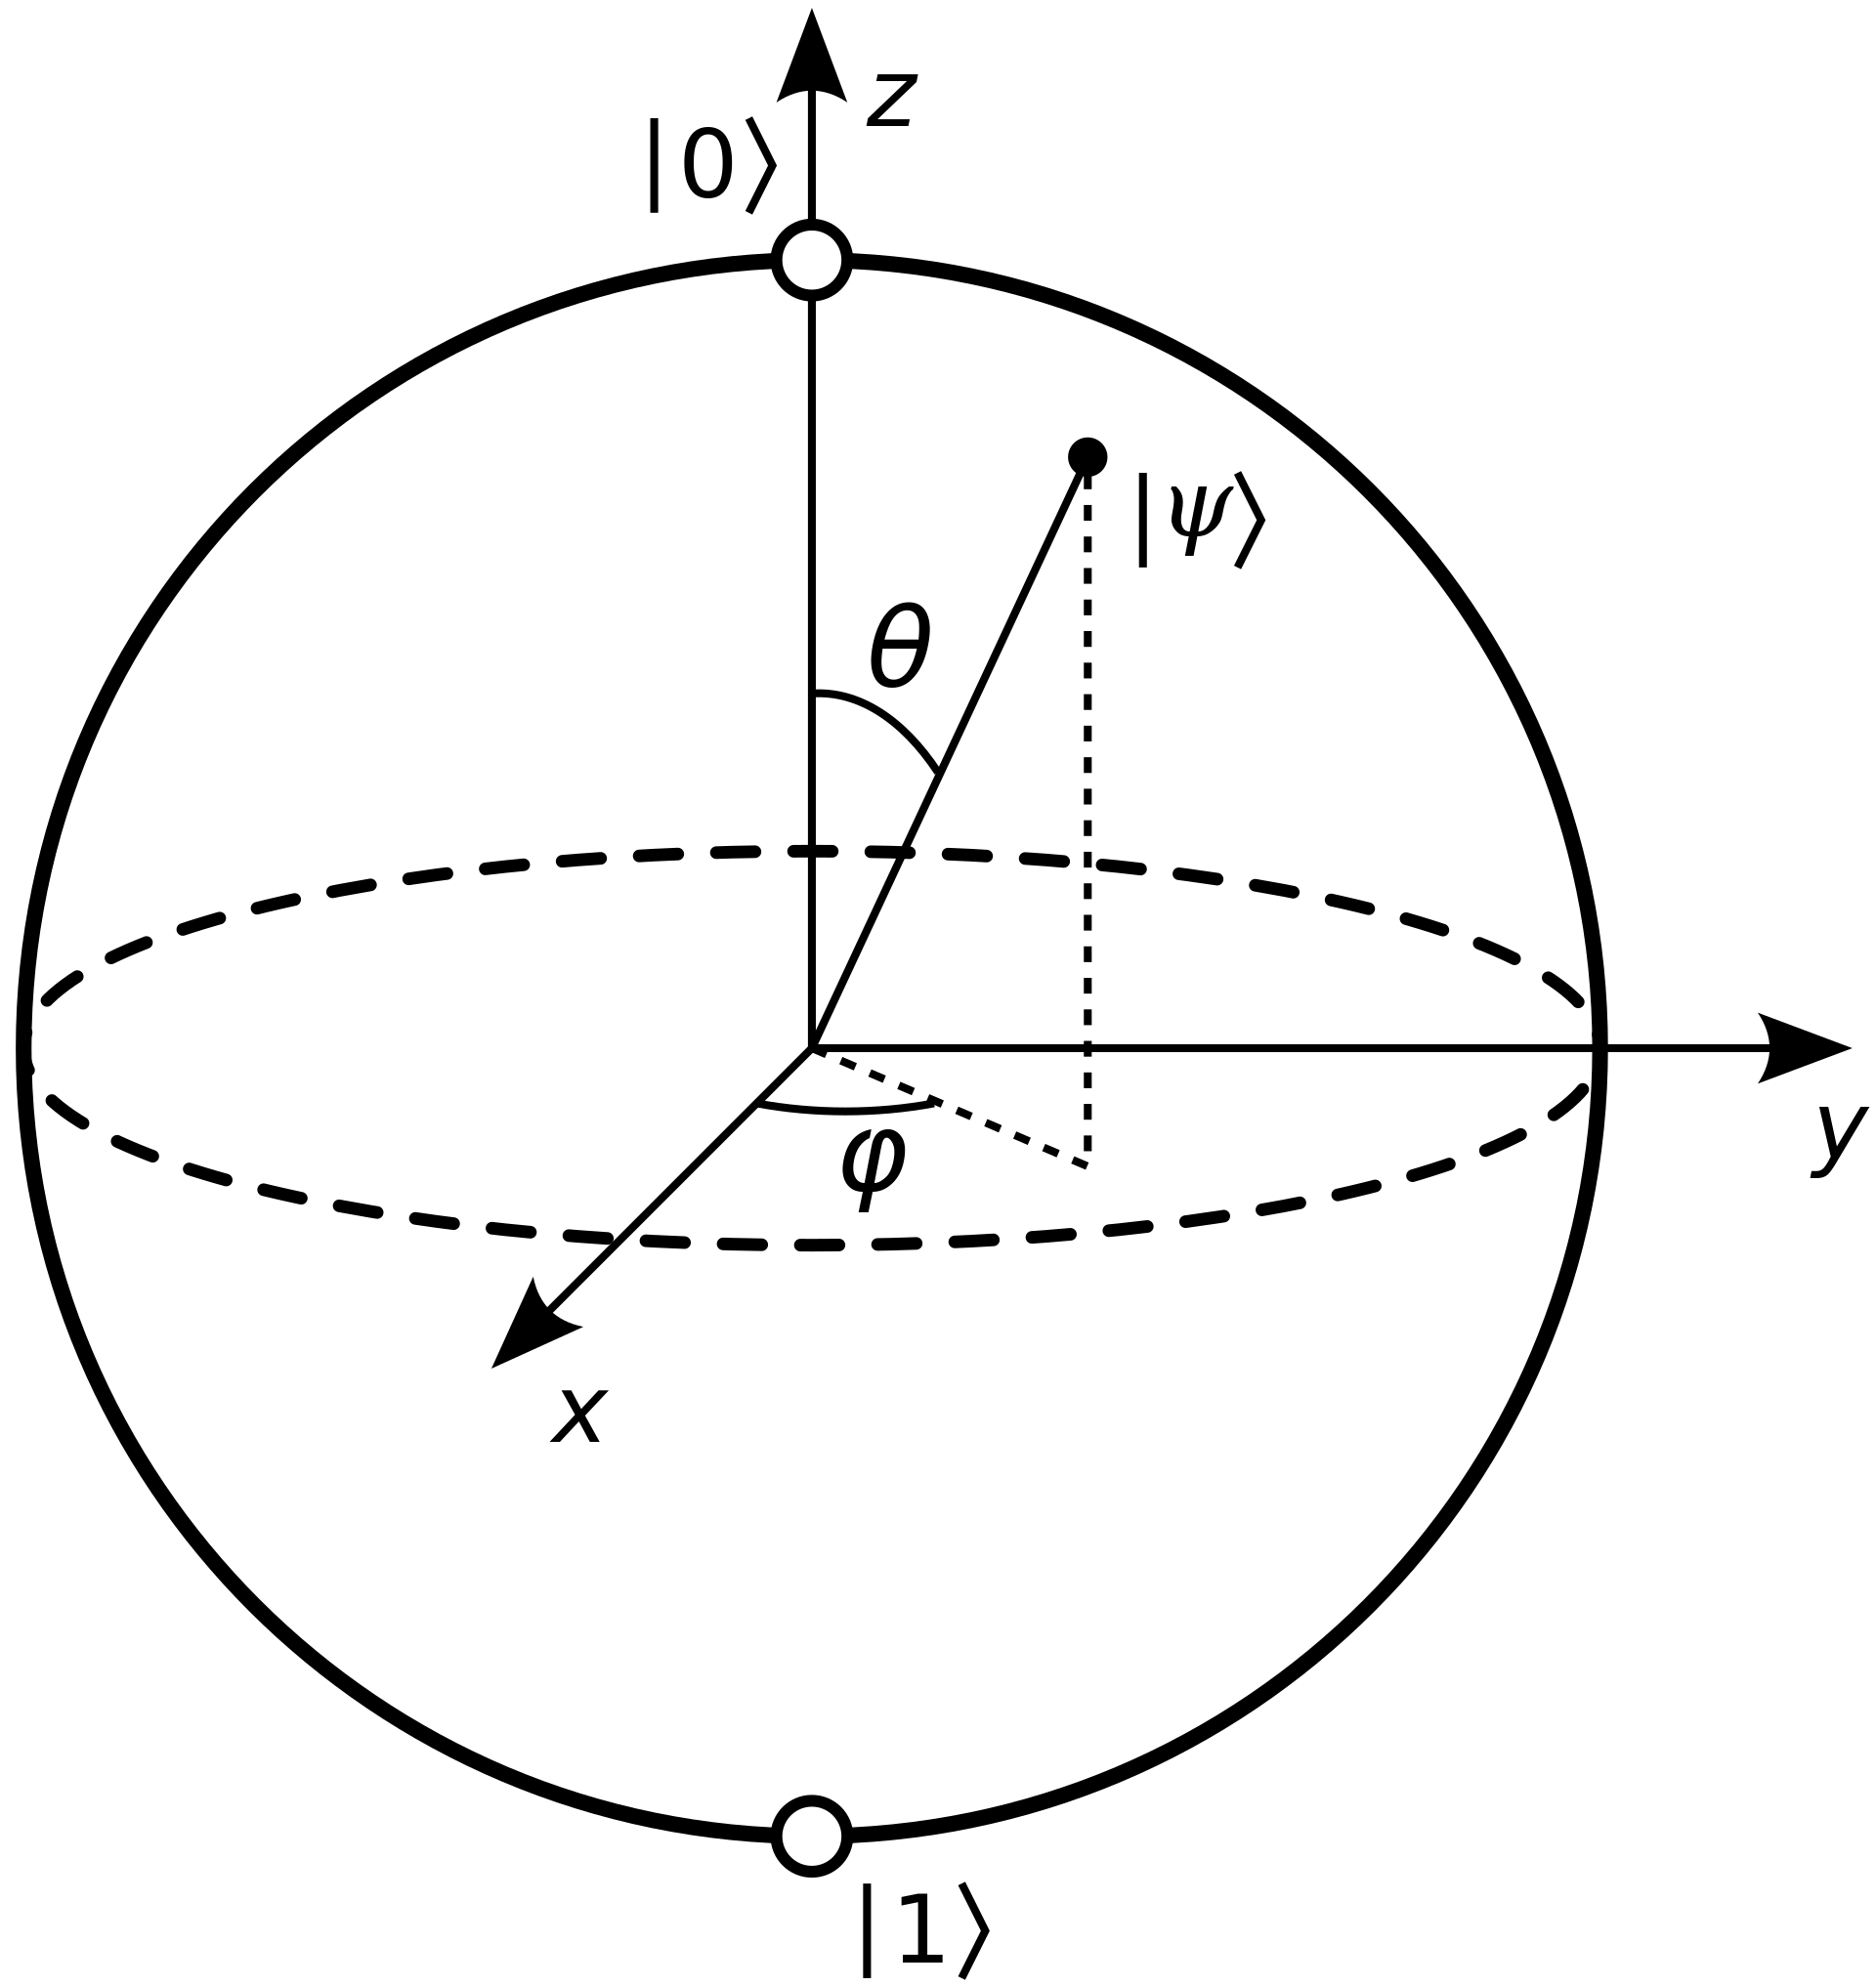
\includegraphics[width=0.5\linewidth]{image/bloch.png}
	\caption{Bloch sphere representation of a qubit. Source: \cite{bloch_sphere_wikipedia}.}
	\label{fig:bloch_sphere}
\end{figure}

\subsection{Multi-qubit State}
Multi-qubit systems are no different from other many-body quantum systems. The combined Hilbert space of $ n $ qubits is the tensor product of the individual Hilbert spaces of each qubit,
\begin{equation}
	\mathcal{H} = \mathcal{H}_1 \otimes \mathcal{H}_2 \otimes \cdots \otimes \mathcal{H}_n.
\end{equation}
The state $ \ket{0 \ldots 0} \equiv \ket{0} \otimes \ket{0} \cdots \ket{0}$ is the tensor product of the $\ket{0}$ states for every Hilbert space. This state is often referred to as the vacuum state of the system. It is worth noting that qubits are assumed to be distinguishable, unlike fermions or bosons. By convention in computer science, the qubit to the right is the first qubit.

\section{Quantum Gates}
\label{sec:quantum_gates}
Mathematically, quantum gates are a series of unitary operators in the operator space $ \mathcal{H} \otimes \mathcal{H}^{*}$ which evolve the state. The unitary nature preserves the norm of the state vector, ensuring the probabilities sum to unity. Since not all gates correspond to an observable, they are not necessarily hermitian. 
\subsection{Single Qubit Gates}
\subsubsection{Pauli Gates}
Pauli gates are Pauli matrices defined in Definition~\ref{def:pauli_matrices}.
\begin{definition}{Pauli Matrices}{pauli_matrices}
    The Pauli matrices are defined as
\begin{equation}
	X \equiv \sigma_x = \begin{pmatrix}
		0 & 1 \\
		1 & 0
	\end{pmatrix}, \quad
	Y \equiv \sigma_y = \begin{pmatrix}
		0 & -i \\
		i & 0
	\end{pmatrix}, \quad
	Z \equiv \sigma_z = \begin{pmatrix}
		1 & 0 \\
		0 & -1
	\end{pmatrix}.
\end{equation}
\end{definition}

The Pauli-X gate is also known as the NOT gate, which flips the state of the qubit.
\begin{align}
	X\ket{0} &= \ket{1}, \\
	X\ket{1} &= \ket{0}.	
\end{align}
The Pauli-Y gate flips the bit and multiplies the phase by $ i $. 
\begin{align}
	Y\ket{0} &= i\ket{1}, \\
	Y\ket{1} &= -i\ket{0}.
\end{align}
The Pauli-Z gate multiplies only the phase of $\ket{1}$ by $ -1 $.
\begin{align}
	Z\ket{0} &= \ket{0}, \\
	Z\ket{1} &= -\ket{1}.
\end{align}

\subsubsection{Hadamard Gate}
The Hadamard gate is defined as
\begin{equation}
	H = \frac{1}{\sqrt{2}} \begin{pmatrix}
		1 & 1 \\
		1 & -1
	\end{pmatrix}.
\end{equation}
It creates a superposition of the $ \ket{0} $ and $ \ket{1} $ states.
\begin{align}
	H\ket{0} &= \frac{1}{\sqrt{2}} \left( \ket{0} + \ket{1} \right), \\
	H\ket{1} &= \frac{1}{\sqrt{2}} \left( \ket{0} - \ket{1} \right).
\end{align}

\subsubsection{Phase Gates}
The S-phase gate is usually denoted as $ S $ and is defined as
\begin{equation}
	S = \begin{pmatrix}
		1 & 0 \\
		0 & i
	\end{pmatrix}.
\end{equation}
It multiplies only the phase of the $ \ket{1} $ state by $ i $.
\begin{align}
	S\ket{0} &= \ket{0}, \\
	S\ket{1} &= i\ket{1}.
\end{align}
Its inverse
\begin{equation}
	S^\dagger = \begin{pmatrix}
		1 & 0 \\
		0 & -i
	\end{pmatrix}
\end{equation}
is known as the $ S^\dagger $ gate which applies a $ -i $ phase shift to \ $ \ket{1}$.
\begin{align}
	S^\dagger\ket{0} &= \ket{0}, \\
	S^\dagger\ket{1} &= -i\ket{1}.
\end{align}

\subsection{Two Qubit Gates}
\subsubsection{CNOT Gate}
\label{ssub:cnot_gate}
The CNOT gate is a two-qubit gate which acts on two qubits, a control qubit and a target qubit. The CNOT gate is defined as
\begin{equation}
	\text{CNOT} = \begin{pmatrix}
		1 & 0 & 0 & 0 \\
		0 & 1 & 0 & 0 \\
		0 & 0 & 0 & 1 \\
		0 & 0 & 1 & 0
	\end{pmatrix}.
\end{equation}
It is often used to perform linear entanglement on qubits.
\begin{align*}
	\label{eq:cnot-behaviour}
	\cnot \ket{00} &= \ket{00}, \\
	\cnot \ket{01} &= \ket{01}, \\
	\cnot \ket{10} &= \ket{11}, \\
	\cnot \ket{11} &= \ket{10}.
\end{align*}
\subsubsection{SWAP gate}%
\label{ssub:swap_gate}
The SWAP gate is a two-qubit gate which swaps the state of two qubits. It is defined as
\begin{equation}
	\text{SWAP} = \begin{pmatrix}
		1 & 0 & 0 & 0 \\
		0 & 0 & 1 & 0 \\
		0 & 1 & 0 & 0 \\
		0 & 0 & 0 & 1
	\end{pmatrix}.
\end{equation}
\begin{align*}
	\swp \ket{00} &= \ket{00}, \\
	\swp \ket{01} &= \ket{10}, \\
	\swp \ket{10} &= \ket{01}, \\
	\swp \ket{11} &= \ket{11}.
\end{align*}


\subsection{Pauli Strings}
A Pauli string, such as $ XIYZ $ is a tensor product of Pauli matrices acting on different qubits. The Pauli string $ XIYZ $ is defined as 
\begin{equation}
	\label{eq:pauli-string-example}
	XIYZ \equiv X_0 \otimes I_1 \otimes Y_2 \otimes Z_3.
\end{equation}
Hamiltonians are often rewritten or decomposed in terms of Pauli string as they can be easily implemented on quantum computers. 

\section{Quantum Circuits}
\label{sec:quantum_circuits}
A quantum circuit is a sequence of quantum gates applied to a set of qubits. 
For example, the Bell state represented by $ \frac{1}{\sqrt{2}} \left( \ket{00} + \ket{11} \right) $  is represented by Figure~\ref{fig:bell_state}~\cite{Nielsen_Chuang_2010}.

\begin{figure}[ht]
	\centering
	\begin{quantikz}
		\lstick{$ \ket{0} $ }  &\gate{H}  &\ctrl{1} &\qw\\
		\lstick{$\ket{0}$}  &\qw   &\targ{} &\qw\\
	\end{quantikz}
	\caption{The quantum circuit which creates the bell state.}
	\label{fig:bell_state}
\end{figure}

\subsection{Quantum Circuit Diagrams}
It is often convenient to represent quantum circuits using quantum circuit diagrams. Table~\ref{tab:qc-diagram} shows the common symbols used to present each component of a quantum circuit.
\begin{table}[ht]
	\centering
	\caption{Quantum Circuit Diagram}
	\label{tab:qc-diagram}

	\begin{tabular}{c c}
		\toprule
	 	Gate & Symbol \\
		\midrule
		$ X $ & \begin{quantikz} & \gate{X} & \end{quantikz} \\
		$ Y $ & \begin{quantikz} & \gate{Y} & \end{quantikz} \\
		$ Z $ & \begin{quantikz} & \gate{Z} & \end{quantikz} \\
		$ H $ & \begin{quantikz} & \gate{H} & \end{quantikz} \\
		$ S $ & \begin{quantikz} & \gate{S} & \end{quantikz} \\
		$ S^\dagger $ & \begin{quantikz} & \gate{S^\dagger} & \end{quantikz} \\
		$ \text{CNOT} $ & \begin{quantikz} & \ctrl{1} & 
					    \\ & \targ{} & \end{quantikz} \\
			$ \text{SWAP} $ & \begin{quantikz} & \swap{1} & \\
					& \targX{} &  \end{quantikz} \\
		\bottomrule
	\end{tabular}
\end{table}


\subsection{Measurement}
\label{sub:measurement}
A measurement is a discontinuous change of the state. A measurement necessarily collapses the state of the qubit to one of the basis states, with probability given by its coefficient. In general, if $  \{ \ket{\psi_j} \} $ is a complete set of basis states, then a measurement on the state $ \ket{\psi} = \sum_{j} c_j \ket{\psi_j} $ in this basis gives a result that can be described as
\begin{equation}
	\ket{\psi} \rightarrow \ket{\psi_j} \quad \text{with probability} \quad |c_j|^2.
\end{equation}
For a product state, the measurement result of any qubit would not affect the states of other qubits, i.e. the probability of each qubit is independent. On an entangled state, for example, a bell state $ \frac{1}{\sqrt{2}} \left( \ket{00} + \ket{11} \right) $, measuring either qubit would collapse the other qubit into the same state. 
The number of times a state is measured in an experiment is commonly known as a ``shot''.

The precision or relative error $ \epsilon $ is defined as 
\begin{definition}{Relative Error}{relative_error}
	If $ a $ is the true value of a quantity and $ a_{meas} $ is the measurement result, then the relative error $ \epsilon $ is defined as 
\begin{equation}
	\label{eq:rel_err}
	\epsilon = \left| \frac{a-a_{meas}}{a} \right|.
\end{equation}
\end{definition}

The number of times a measurement is repeated is called the number of shots. In general, a precision of $ \epsilon $ requires $ \mathcal{O}(1/\epsilon^2) $ shots as a result of statistics~\cite{knill2007}.

\section{Fermionic Encoding}
One key consequence of the Pauli exclusion principle is that no two fermions can occupy the same quantum state, which means a state in a fermionic system can be represented by a binary string. One could map the fermionic creation and annihilation operators to gates as long as the mapping has the same commutation relation.

\subsection{Jordan-Wigner Transformation}
\label{sub:jw}
The Jordan-Wigner transformation is a mapping between fermionic operators and spin operators~\cite{Jordan1993, Seeley2012}. 
If $ \hat a_n^{\dagger} $ is the creation operator for the $n$th fermion,
\begin{equation}
	\label{eq:jw}
	\begin{aligned}	
		\hat a^{\dagger}_n &\mapsto \frac{1}{2} \left[ \prod_{j=0}^{n-1} -Z_j \right] \left( X_n - i Y_n \right), \\
		\hat a_n &\mapsto \frac{1}{2} \left[ \prod_{j=0}^{n-1} -Z_j \right] \left( X_n + i Y_n \right). 
	\end{aligned}
\end{equation}

\subsection{Pauli Decomposition}
The Pauli matrices $\sigma_x (X), \sigma_y (Y), \sigma_z (Z)$, together with the identity operator $ I $ in the space of two by two matrices $ \mathcal{M}_{2\times 2} $ form a complete set of basis in $ \mathcal{M}_{2\times2} $. The tensor products of these operators form complete basiss in the of $ \mathcal{M}_{2^n \times 2^n} $.
If the Hamiltonian $ \hat H $ of a system is given by a $ 2^n \times 2^n $ matrix, 
it could be mapped to qubit space using 
\begin{equation}
	\label{eq:pauli-decomp}
	\hat H_{\text{qubit}} =
	\sum_{\mathcal{P}} \frac{1}{2^n} Tr{\left( \mathcal{P} \hat H \right)},
\end{equation}
where $ \mathcal{P} $ is a Pauli string in $ 2^n \times 2^n $.

This uses only $ \lceil \log_2{n} \rceil $ qubits to map a $ 2^n \times 2^n $ matrix. 


\section{Quantum Algorithms}
\label{sec:quantum_algorithms}

\subsection{Variational Quantum Eigensolver}
\label{sub:vqe}

\begin{figure}[ht]
    \centering
    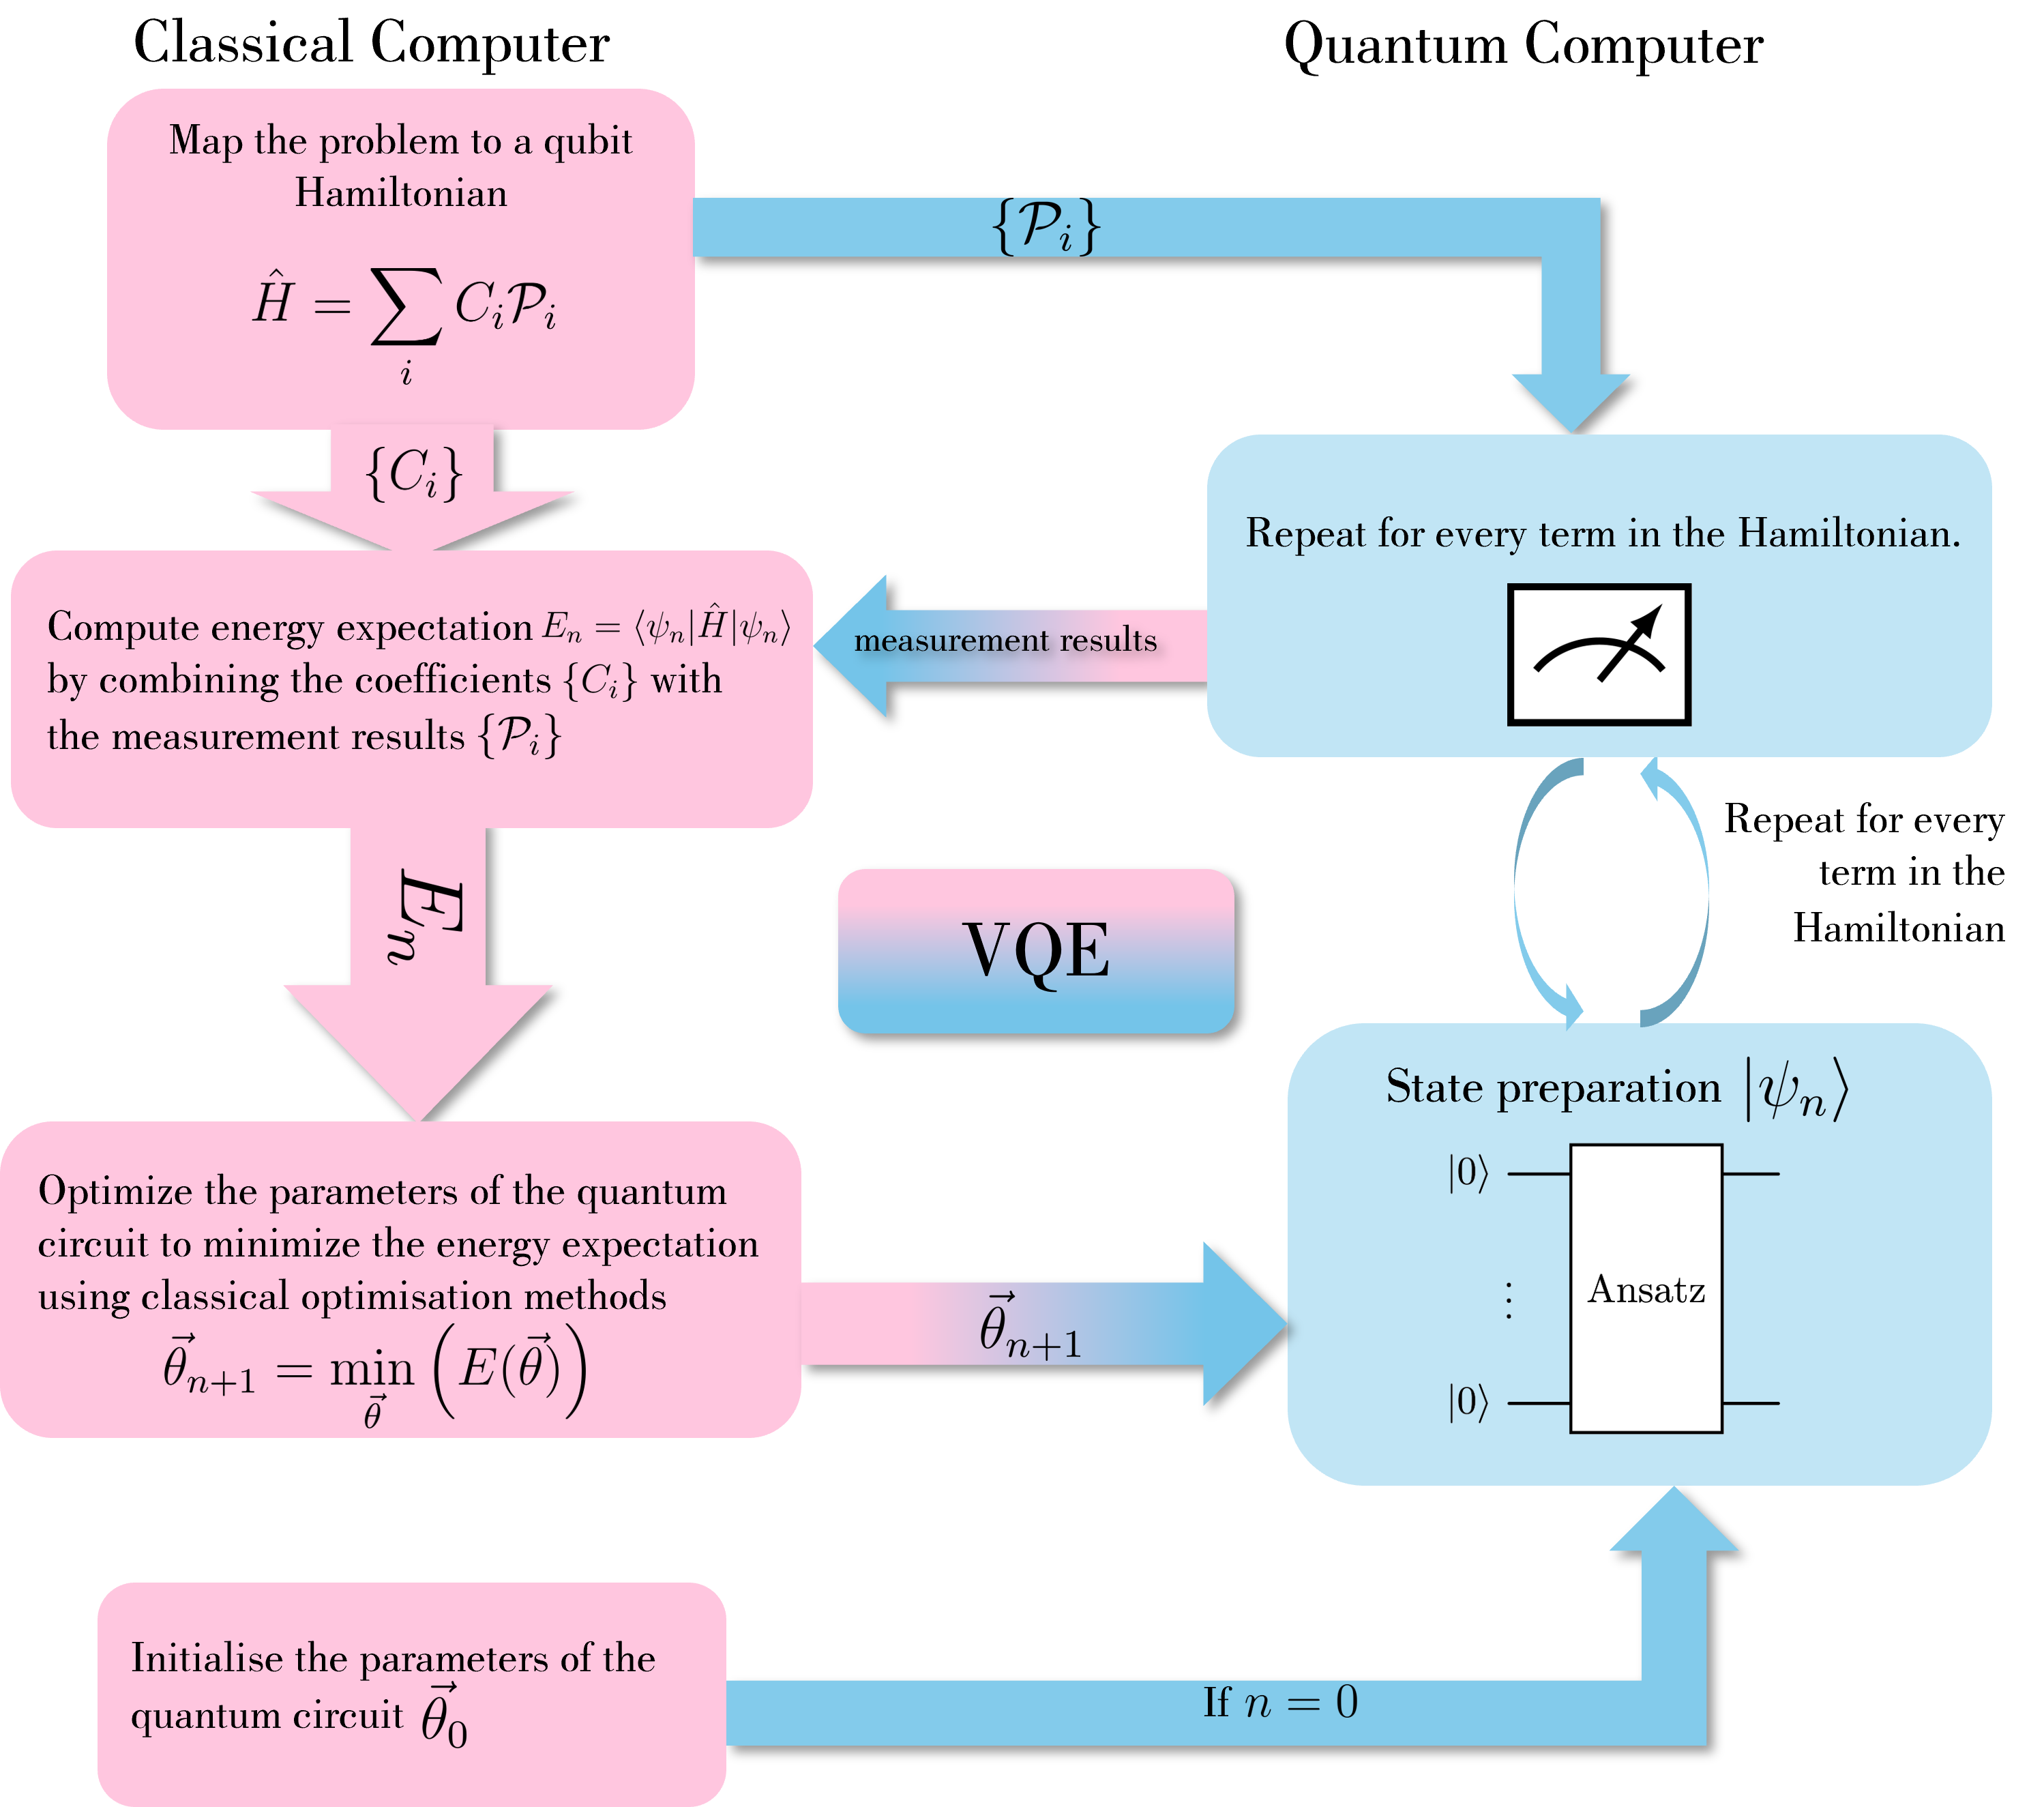
\includegraphics[width=0.7\linewidth]{image/vqe-illu.png}
    \caption{Illustration of the VQE algorithm.}
    \label{fig:vqe-illu}
\end{figure}

The variational quantum eigensolver is a hybrid quantum algorithm that can be realised on a NISQ quantum computer. It consists of an ansatz which is a parameterised circuit. The ansatz prepares a state which is then measured to estimate the energy expectation value. This is the objective function for the classical optimiser which updates the parameter iteratively to find the optimal parameter which minimises the energy utilising the variational principle~\cite{peruzzo2014}. The VQE algorithm is illustrated in Figure~\ref{fig:vqe-illu}. The hybrid and variational nature of the algorithm allows it to be run on NISQ devices and the classical optimisation reduces the length and depth of the quantum circuit.

\subsubsection{Barren Plateaus}
\label{sub:barren_plateaus}
The VQE algorithm amongst many other hybrid quantum algorithms relies on doing optimisation classically and often uses what is called a \textit{Random Parameterised Quantum Circuit(RPQC)} with the form 
\begin{equation}
	\label{eq:rpqc}
	U(\vec{\theta}) = U(\theta_1 \ldots \theta_L) \prod_{l=1}^{L}  U_l(\theta_l) W_l,
\end{equation}
where $ U_l(\theta_l)$ is the parameterised unitary operator of the circuit and $ W_l $ is the unitary operator that does not depend on any parameter. Take the hardware efficient ansatz circuit from Figure~\ref{fig:4hw} as an example: the $ U_l $ would be the single qubit rotation gates and the $ W_l $ would be the CNOT gates, as shown in Figure~\ref{fig:UandW in rpqc}.
\begin{figure}[ht]
	\centering	
	\begin{quantikz}
    \lstick{$q_0$} & \gate{Rx(\theta_0)}\gategroup[4,steps=2,style={inner sep=6pt}]{$U_l$}&\gate{Ry(\phi_0)}&
    \ctrl{1} &\qw &\qw &\qw &\\
\lstick{$q_1$} &\gate{Rx(\theta_1)} &\gate{Ry(\phi_1)} & \targ{}  &\ctrl{1} &\qw &\qw \\
\lstick{$q_2$} & \gate{Rx(\theta_2)} & \gate{Ry(\phi_2)}& \qw &\targ{} &\ctrl{1} &\qw\\
\lstick{$ q_3 $} & \gate{Rx(\theta_3)} & \gate{Ry(\phi_3)}& \qw & \qw & \targ{} &\qw
\end{quantikz}
	\caption{The $ U_l $ and $ W_l $ in a RPQC.}
	\label{fig:UandW in rpqc}
\end{figure}

This is a common form for the ansatz because it allows easy calculations of the gradients
\begin{equation}
	\label{eq:gradient}
	\frac{\partial E\left( \vec{\theta} \right) }{\partial \theta_l} = \frac{\partial \braket{\psi(\vec{\theta})|H|\psi(\vec{\theta})}}{\partial \theta_l} =
	i\braket{0\left|U_{-}^{\dagger}\left[V_k, U_{+}^{\dagger} H U_{+}\right] U_{-}\right| 0},
\end{equation}
where $U_{-} \equiv \prod_{l=0}^{k-1} U_l\left(\theta_l\right) W_l$ and $U_{+} \equiv \prod_{l=k+1}^{L} U_l\left(\theta_l\right) W_l$ \cite{mcclean2018}.
Mcclean et al. also showed that for a large number of random circuits, the average value of the gradient and the variance of the gradient decrease exponentially with the number of qubits~\cite{mcclean2018}. Unlike classical deep neural networks, which scale as $ \mathcal{O}(log(1/\epsilon)) $, the cost of estimating the gradient scales with $ \mathcal{O}(\frac{1}{\epsilon^\alpha})$ where $ \epsilon $ is the deviation from the average value desired and $ \alpha $ is arbitrarily small. The optimisation process is akin to a random walk if $ \epsilon $ is the size of the gradient and the number of measurements is not on the order of $ 1/ \epsilon^{\alpha}$. 
This phenomenon is known as the barren plateau problem, as the gradient has an exponentially small probability of random walking out of the plateau~\cite{mcclean2018}.


\subsubsection{Second Quantised Hamiltonian}%
\label{ssub:second_quantised_hamiltonian}
The Hamiltonians we try to solve with VQE are usually with Hamiltonians in the form of Equation~\eqref{eq:sq_hamiltonian}.

\begin{equation}
	\label{eq:sq_hamiltonian}
	\hat H = \sum_{pq} h_{pq} \hat a_p^\dagger \hat a_q + { \frac{1}{2} \sum_{pqrs} h_{pqrs} \hat a_p^\dagger \hat a_q^\dagger \hat a_r \hat a_s},
\end{equation}
where $ h_{pq} $ and $ h_{pqrs} $ are the one- and two-body integrals, given by 
\[\braket{p|\hat h_0|q}, \] 
and 
\[ \braket{pq|\hat V|rs}, \] 
where $ \hat h_0 $ is the one-body operator and $ \hat V $ is the two-body (interaction) operator.


\subsection{Ansatz}
\label{sub:ansatz}
The form of the ansatz for the VQE is crucial for the convergence of the VQE. A good ansatz should be able to represent the ground state of the system, so that convergence to the ground state energy is possible; span only the necessary section of the Hilbert space, thus reducing the optimisation complexity; as well as be shallow, since we are still in the NISQ era. 

\subsubsection{Hardware Efficient Ansatz}%
\label{ssub:hardware_efficient_ansatz}
A hardware efficient ansatz is a class of ansatzes that uses single qubit rotation gates and linear entanglement CNOT gates that are available to quantum computers~\cite{park2024}. Figure~\ref{fig:4hw} illustrates an example circuit for a hardware efficient ansatz with four qubits. The single qubit rotation gates are parameterised and these parameters are optimised classically to search for the minimum. Note that there could be many other different kinds of hardware efficient ansatz, such as the RyRz ansatz, which uses Ry and Rz gates, or the Ry ansatz, which uses only Ry gates. 
\begin{figure}[ht]
	\centering
	\begin{quantikz}
		\lstick{$q_0$}  &\gate{Rx(\theta_0)}   &\gate{Ry(\phi_0)} &\ctrl{1} &\qw &\qw &\qw &\qw\\
		\lstick{$q_1$}  &\gate{Rx(\theta_1)}   &\gate{Ry(\phi_1)} &\targ{} &\qw &\ctrl{1} &\qw &\qw \\
		\lstick{$q_2$}  &\gate{Rx(\theta_2)}   &\gate{Ry(\phi_2)} &\qw &\qw &\targ{} &\ctrl{1} &\qw\\
		\lstick{$q_3$}  &\gate{Rx(\theta_3)}   &\gate{Ry(\phi_3)} &\qw &\qw &\qw  &\targ{} &\qw \\
	\end{quantikz}
	\caption{Example of the hardware efficient ansatz in a our-qubit circuit.}
	\label{fig:4hw}
\end{figure}

The hardware efficient ansatzes usually have relatively short circuits compared to other ansatzes and are easy to implement on quantum computers since they consist only of gates that are directly available on the hardware. One downside of the hardware efficient ansatz is that there is no information about the Hamiltonian we are trying to solve, and since the ansatz does not exhaust the entire Hilbert space nor should it, it may not be able to represent the ground state of the system. However, it is almost always a good starting point due to the simplicity of the ansatz and serves as a good benchmark for more complex ansatz. 
Although it seems like an ab initio approach, the hardware efficient ansatz can actually successfully represent the ground state of many systems, as we will show in Chapter~\ref{chap:results}. The reason why this worked at all is since the hardware efficient ansatz consists of rotation gates \texttt{Rx, Ry, Rz} and CNOT gates, and these gates form a universal gate set. According to the Solovay-Kitaev theorem, any unitary operator can be approximated to arbitrary precision using a finite number of gates from a universal gate set~\cite{Kitaev1997}. This means that the gates involved in the hardware efficient ansatz can theoretically represent any unitary operator, and thus any state in the Hilbert space. 

\subsection{Adaptive, Problem Tailored VQE}
\label{sub:adapt_vqe}
Grimsley et al. proposed the Adaptive, Problem Tailored VQE (ADAPT-VQE) algorithm~\cite{grimsley2019} which aims to provide an adaptive ansatz structure which can capture information about the Hamiltonian.
The ADAPT-VQE uses an evolving ansatz which is updated at every iteration by appending a new operator onto the circuit chosen from a predefined operator pool without draining the pool. The ADAPT-VQE consists of the following steps:
\begin{enumerate}
	\item Define an operator pool$ \ \{ A \}  $ . 
	\item Calculate the gradient of energy with respect to each operator in the pool.
	\item Select the operator with the largest gradient, $ A $ , append $ e^{\theta A} $ onto the circuit.
	\item Optimise all the parameters in the circuit using VQE.
	\item Repeat steps 2 to 4 until the gradient of all operators is below a threshold.
\end{enumerate}
An ADAPT iteration is defined by steps two to four.
After $ n $ ADAPT iterations, the ansatz should look like:
\[ \ket{\psi_{n}} = e^{\theta_0 A_0} e^{\theta_1 A_1} \ldots e^{\theta_n A_n}\ket{\psi_{0}}. \] 
\subsubsection{Selection Criteria}%
\label{ssub:selectioncriteria}
Steps 2 and 3 of the Adapt VQE require the calculation of the gradient of the energy with respect to the new parameter.
The gradient of the operator $ \left(\frac{\partial E}{\partial \theta}\right)_{\theta = 0} $ is given by:
\begin{align}
	\label{eq:A-gradient}
	\left( \frac{\partial E}{\partial \theta} \right)_{\theta = 0} &= \left( \frac{\partial }{\partial \theta} \right) \braket{\psi_n|e^{-\theta A}H e^{\theta A}|\psi_n}_{\theta = 0}, \\
	&= \braket{\psi_n|\left( -A e^{-\theta A} H e^{\theta A}\right)  + \left( e^{-\theta A}HAe^{\theta A} \right)|\psi_n }_{\theta=0}, \\
	&= \braket{\psi_n|-AH + HA|\psi_n}, \\
	&= \braket{\psi_n|[H,A]|\psi_n}.
\end{align}
The operator $ e^{\theta A_i} $ will be appended if 
\begin{equation}
	\label{eq:selection-criteria}
	\left( \frac{\partial E}{\partial \theta_i}\right)_{\theta_i = 0} > \left( \frac{\partial E}{\partial \theta_j} \right)_{\theta_j = 0}, \quad \forall A_j \in \{A\}. 
\end{equation}
The ADAPT-VQE algorithm is illustrated in Figure~\ref{fig:adapt-illu}.

\begin{figure}[ht]
    \centering
    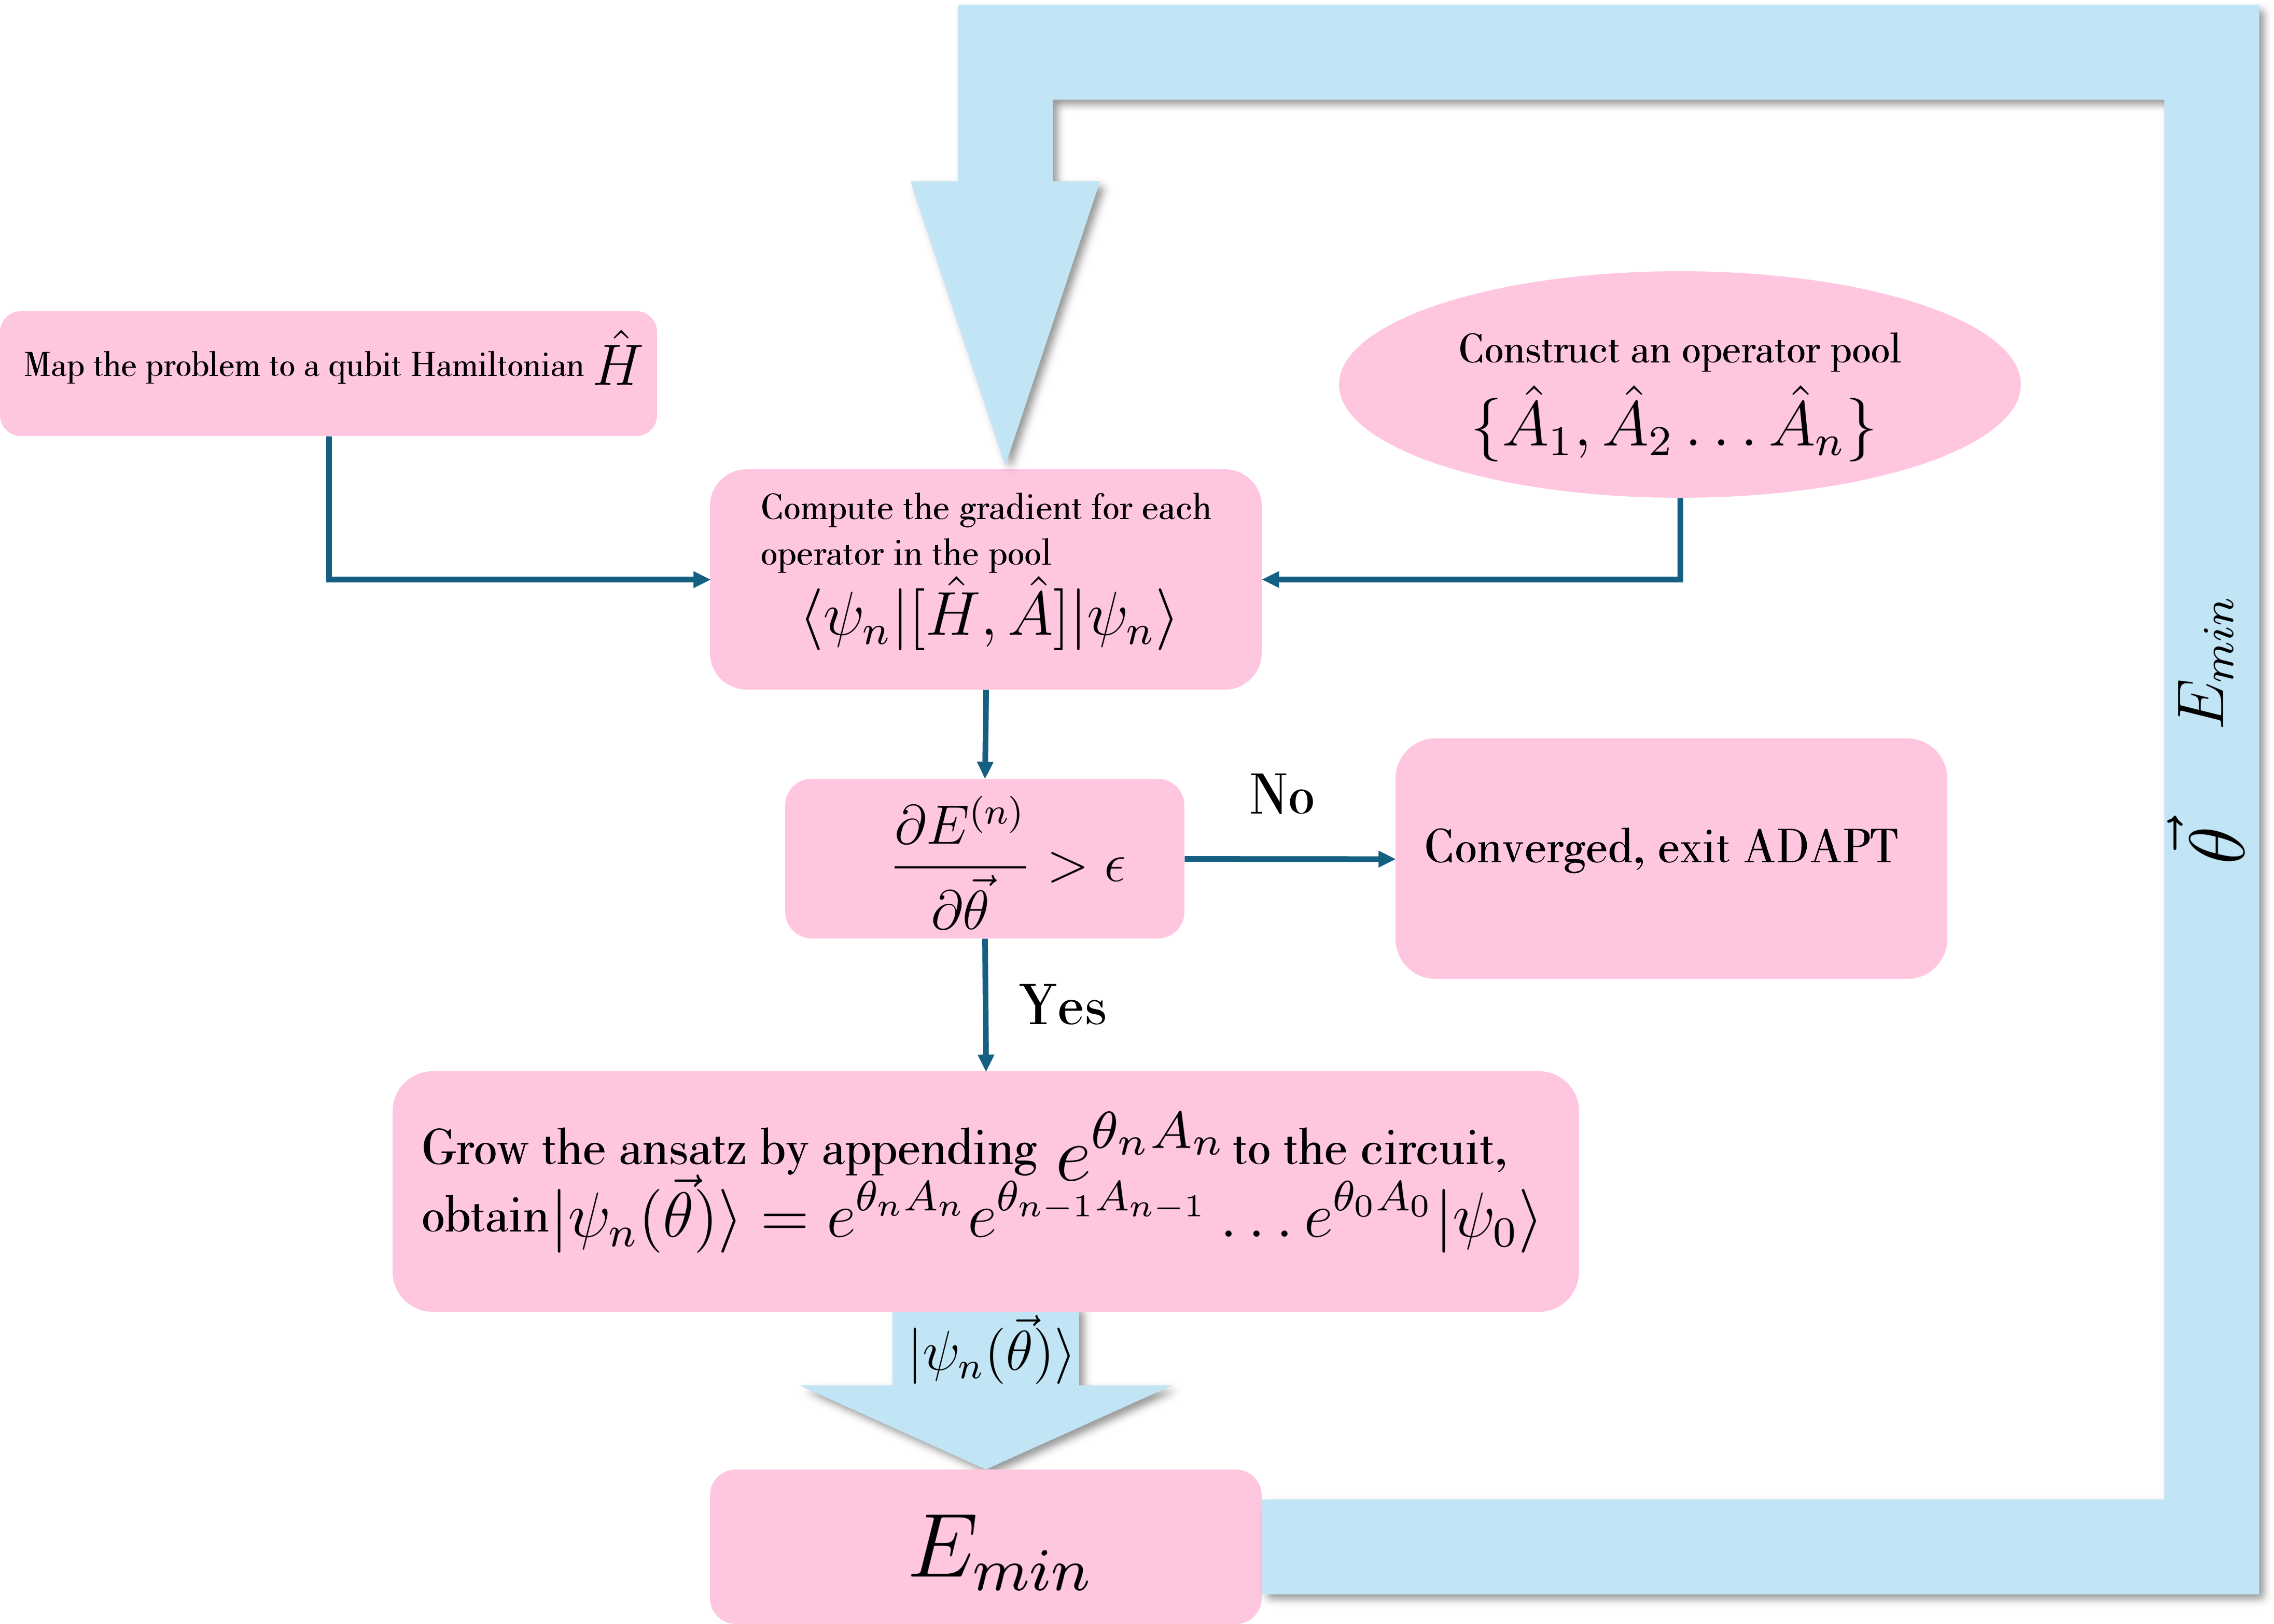
\includegraphics[width=0.8\linewidth]{image/adapt-illu.png}
    \caption{Illustration of the ADAPT-VQE algorithm.}
    \label{fig:adapt-illu}
\end{figure}


\subsection{qubit-ADAPT-VQE}
\label{sub:qubit_adapt_vqe}
The qubit-ADAPT-VQE is a hardware efficient variant of the ADAPT-VQE where the operator pool is chosen to contain only odd Pauli strings, i.e. Pauli strings with odd numbers of Y operators. Since in the case where the Hamiltonian has time-reversal symmetry, the Hamiltonian is real, choosing imaginary Pauli strings causes the analytical expression of the gradient given in Equation~\eqref{eq:A-gradient} to vanish. By choosing only odd operators the ansatz also stays real throughout the ADAPT iterations. A complete pool is defined as a pool that can transform the reference state to any real state. To create any arbitrary real state in the $ n $ qubit Hilbert space requires only $ 2^n -1 $ real parameters.
If $ \{ A_i \}  $ is such that for any arbitrary state $ \ket{\psi}$,  $A_i \ket{\psi}$ form a complete basis, then $ \{ A_i \}  $ is referred to as a complete basis of operators. The minimum size of a complete pool for $ n $ qubit has size $ 2n-1 $, which scales only linearly in number of qubits~\cite{tang2021}. 

We will present the two families of minimal complete pools proven by~\cite{tang2021} and refer to them as the $ V $ pool and $ G $ pool from now on. A family of complete operator pools, $ \{ V_j \}_n $,  where $ V_j $ is an operator in the pool and $ n $ is the number of qubits, can be constructed recursively as follows,
\begin{align}
\label{eq:vpool}
\{ V_j \}_2 = &\{ iY_1Z_2, \ iI_1Y_2 \}, \\
\{ V_j \}_n = &\{\{V_k\}_{n-1}Z_n, \ iI_1I_2 \ldots Y_n, \ iI_1I_2 \ldots Y_{n-1} I_n. \}
\end{align}
	The $ \{ V_j \}_n $ can be mapped onto a different family of operator pool, $ \{ G_j \}_n  $ which contains $ iY $ on every single qubit and two-qubit operator $ iY_kZ_{k+1} $ on adjacent qubits $ k $ and $ k+1 $,  
\begin{align}
\label{eq:gpool}
\{ G_j \}_n = &\{ iY_1I_2 \ldots I_n, \ iI_1Y_2 \ldots I_n, \ \ldots, \ iI_1 \ldots I_{n-1}Y_n, \\
              & iY_1Z_2I_3 \ldots I_n, \ iI_1Y_2Z_3I_4 \ldots I_n, \ \ldots, \ iI_1 \ldots I_{n-2}Y_{n-1}Z_{n}. \}
\end{align}



\part{Implementation}
\chapter{Quanthon: Quantum Computing in Python}
\label{ch:quanthon}

This chapter details the design and implementation of a quantum computing library in Python~\cite{python3}, namely \texttt{Quanthon}. The library can be found at \url{https://pypi.org/project/Quanthon/} and the source code at \url{https://github.com/moyasui/Quanthon}.

While existing quantum computing libraries such as Qiskit~\cite{qiskit}, and Circ~\cite{cirq_2024} are usually better integrated with hardware, more optimised and contain more functionalities, writing an entire library from scratch can be beneficial pedagogically by forbidding the existence of black boxes as well as allowing more freedom in structures and conventions. One example of such is the ordering of qubits. Let $ A, B,C,D $ be single-qubit operations, most literature uses $ ABCD $ to mean $ A_1B_2C_3D_4 $ i.e. applying the gate $ A $ on the first qubit, $ B $ on the second etc. This, however, is inconsistent with the computer science convention of representing numbers using bit strings, where the most significant bit is to the left. For example, the decimal $ 4 $ is usually written as $ 100 $ in binary representation. Most quantum computing libraries adhere to the binary representation convention by having the most significant bit to the left, therefore logically the aforementioned 4-qubit gate should have been written as $ DCBA $, which sadly is not. There is no physical reason for this choice and it is purely conventional, hence no reason to compromise for it. In Quanthon, the most significant bit is to the right, and the order of operators/gates is written normally, in the same order.  

Quanthon is also designed to be minimalistic and with the focus of physicists in mind. The library is designed to be used for quantum simulations and solving physical problems, following the most fundamental principles rather than specialising in, e.g.\ electronic systems. The library is also designed to be easily extensible, with the ability to add custom gates and operators, algorithms and models. 

Quanthon will continue to be maintained and expanded after the conclusion of this master's project. 

\newpage

\section{Architecture}
\label{sec:arch}
\begin{figure}[ht]
	\centering
	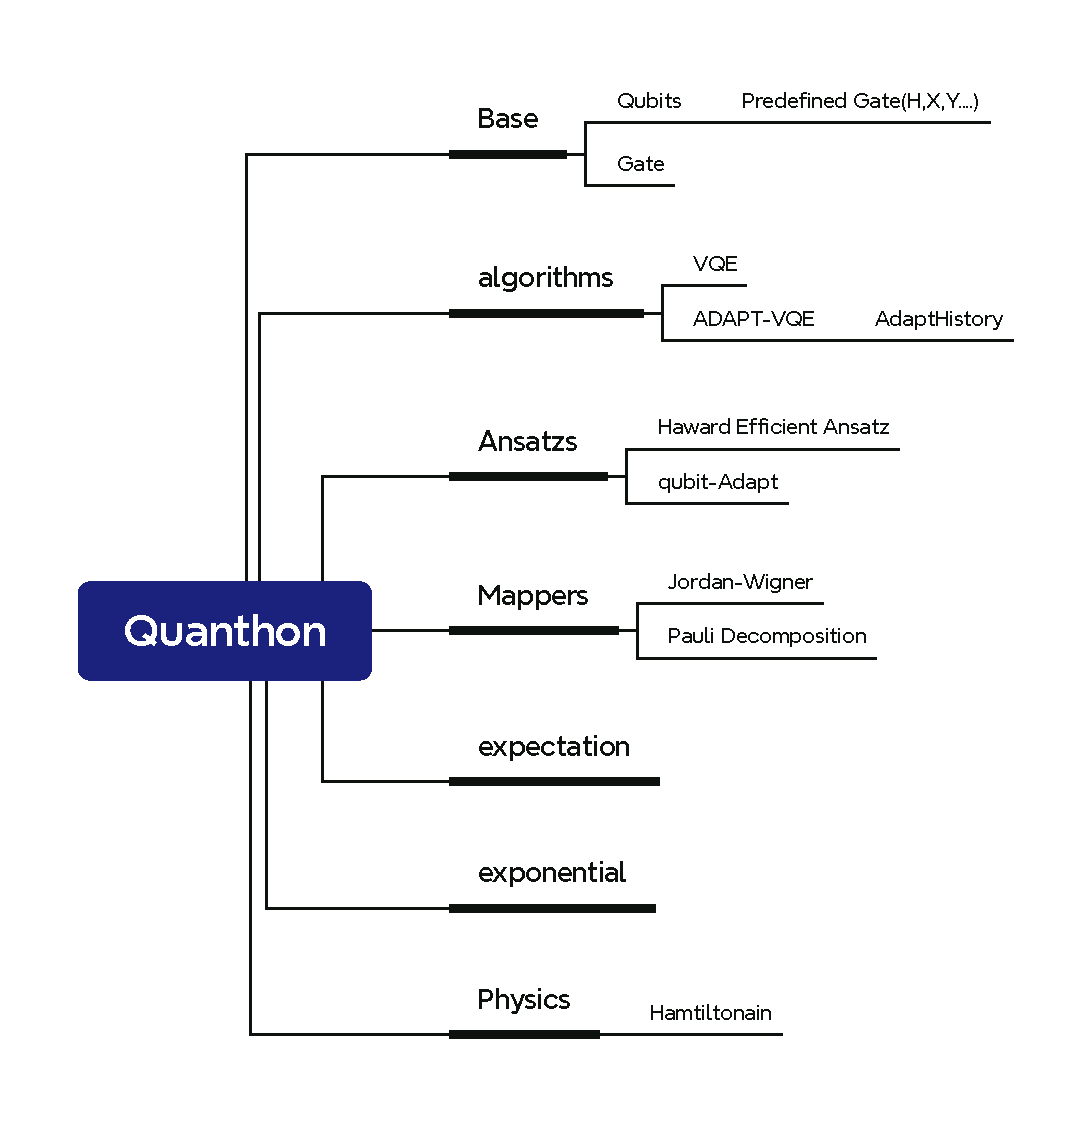
\includegraphics[width=\textwidth]{image/architecture.pdf}
	\caption{Architecture of Quanthon.}
	\label{fig:image-architecture}
\end{figure}

Figure~\ref{fig:image-architecture} shows the architecture of Quanthon. Quanthon is built with quantum simulations and solving physical problems in mind, and it is divided into a few modules and several standalone functions. The basic module is the \texttt{base} module, this is where all the circuitry and gates are defined. The \texttt{algorithms} and \texttt{Ansatz} are heavily focused on the Variational Quantum Eigensolver. The \texttt{expectation} module contains functions that calculate the expectation value of an operator and \texttt{exponential} creates a circuit which exponentiates a Pauli string. The \texttt{Physics} module is used for storing the integrals of a second quantised Hamiltonian. The \texttt{Mappers} contains functions for transforming the Hamiltonian from different forms in terms of Pauli operators. The \texttt{utils} and \texttt{mappers\_utils} modules contain helper functions.

\newpage
\section{Basic Elements of Quantum Computing}
\label{sec:base}
In theory, all quantum computation can be simulated using only these basic elements we introduce in this section, qubits and gates as described in Chapter~\ref{ch:qc}. 
This section explains the structure for \texttt{base.py}, including the \texttt{Gate} class and \texttt{Qubits} class.
\subsection{Qubits}
\label{sub:qubits}
A \texttt{Qubits} object is the most fundamental unit for quantum computation. It contains information about
\begin{itemize}
	\item the number of qubits, \texttt{Qubits.n\_qubit},
	\item the current circuit, \texttt{Qubits.circuit},
	\item the current state of the qubits, \texttt{Qubits.state},
	\item the history of all the gates applied to the circuit, which is not cleared when the circuit is reset \texttt{Qubits.gate\_history},.
\end{itemize}

Initialise a \texttt{Qubits} object of $ 2 $ qubits to the $ \ket{0} $ state by calling
\begin{mycode}
	from Quanthon import Qubits
	q = Qubits(2)
\end{mycode}
 

To manipulate the circuit by appending gates to the circuit,
\begin{mycode}
	q.H(0) # appends the Hadamard gate (a \texttt{Gate} object) on the $ 0th $ qubit to q.circuit. \
	q.CNOT(0,1) # appends the CNOT with control qubit $ 0 $  and target qubit $ 1 $ to q.circuit. \
	q.run() # apply all the gates in q.circuit
	q.draw() # generate code for drawing the circuit in Quantikz~\cite{kay2023tutorialquantikzpackage}.
\end{mycode}
Below we list all currently available gates as methods of the \texttt{Qubits} class
\begin{itemize}
	\item \texttt{H} (Hadamard gate), 
	\item \texttt{X,Y,Z} (Pauli matrices),
	\item \texttt{Rx, Ry, Rz} (single qubit rotation gates),
	\item \texttt{Sdag}, $ S^{\dagger}$, the Hermitian conjugate of the S-phase gate,
	\item  \texttt{CNOT} (controlled-not) gate,
	\item \texttt{SWAP} (the swap gate).
\end{itemize}
To simulate a classical measurement with $ n $ shots, where the probability is given by amplitude squared using the Born rule.
\begin{mycode}
	counts = q.measure(n_shots=10000)
\end{mycode}
where \texttt{count} contains the simulated result for $ 10000 $ shots of the same circuit \texttt{q}. The output is a $ 2^n \times 2 $ array, the first column is the count corresponding to the state in binary in the second column.

\begin{mycode}
>>> counts
array([[5025, '00'],
       [0, '01'],
       [0, '10'],
       [4975, '11']], dtype=object)
\end{mycode}
Other available methods that could be useful include
\begin{itemize}
	\item \texttt{reset} to reset the state of the qubits to $ \ket{0} $,
	\item \texttt{set\_state} which sets the state of the qubits to a given state, also checks if the state is valid,
	\item \texttt{reset\_circuit} which resets the circuit to an empty list,
	\item \texttt{copy} which returns a copy of the \texttt{Qubits} object with the same states but not gates in the circuit, this is useful when repeated circuit preparation is needed for measurement,
	\item \texttt{\_to\_comp\_basis} which returns the state in the more readable bra-ket notation when the print statement is called. For example, the following code gives
\begin{mycode}
	>>> q = Qubits(2)
	>>> print(q)	
\end{mycode} 
	\[ \text{Qubit(s) in state:} 1.00+0.00j\ket{00} \]
	\item \texttt{count\_gates} which returns the length of the circuit
	\item \texttt{count\_cnots} which returns the number \cnot gates currently in the circuit.
	\texttt{draw} provides visualisation of the circuit and returns a Quantikz \missingref string that represents the circuit.
\end{itemize}


\subsection{Shot Noise}%
\label{sub:shot_noise}
In this section, we will numerically show the error of state tomography for different numbers of shots and compare their precisions. We first prepare a state $ \ket{\psi}  $ such that
\[ \ket{\psi} = \frac{1}{2} \left( \ket{00} + \ket{01} + \ket{10} + \ket{11} \right)  \] 
We now measure the state $ \ket{\psi} $ for $ [4^2, 4^3, 4^4, 4^5, 4^6, 4^7, 4^8, 4^9]$ shots and compare the error, as well as to the theoretical result from Subsection~\ref{sub:measurement}. If the precision required is $ \epsilon $ then the number of shots required $ \propto \frac{1}{\epsilon^2} $. Then every time the number of shots is increased by a factor of four, the error should be reduced by a factor of $\frac{1}{2}$. 
\begin{figure}[ht]
	\centering
	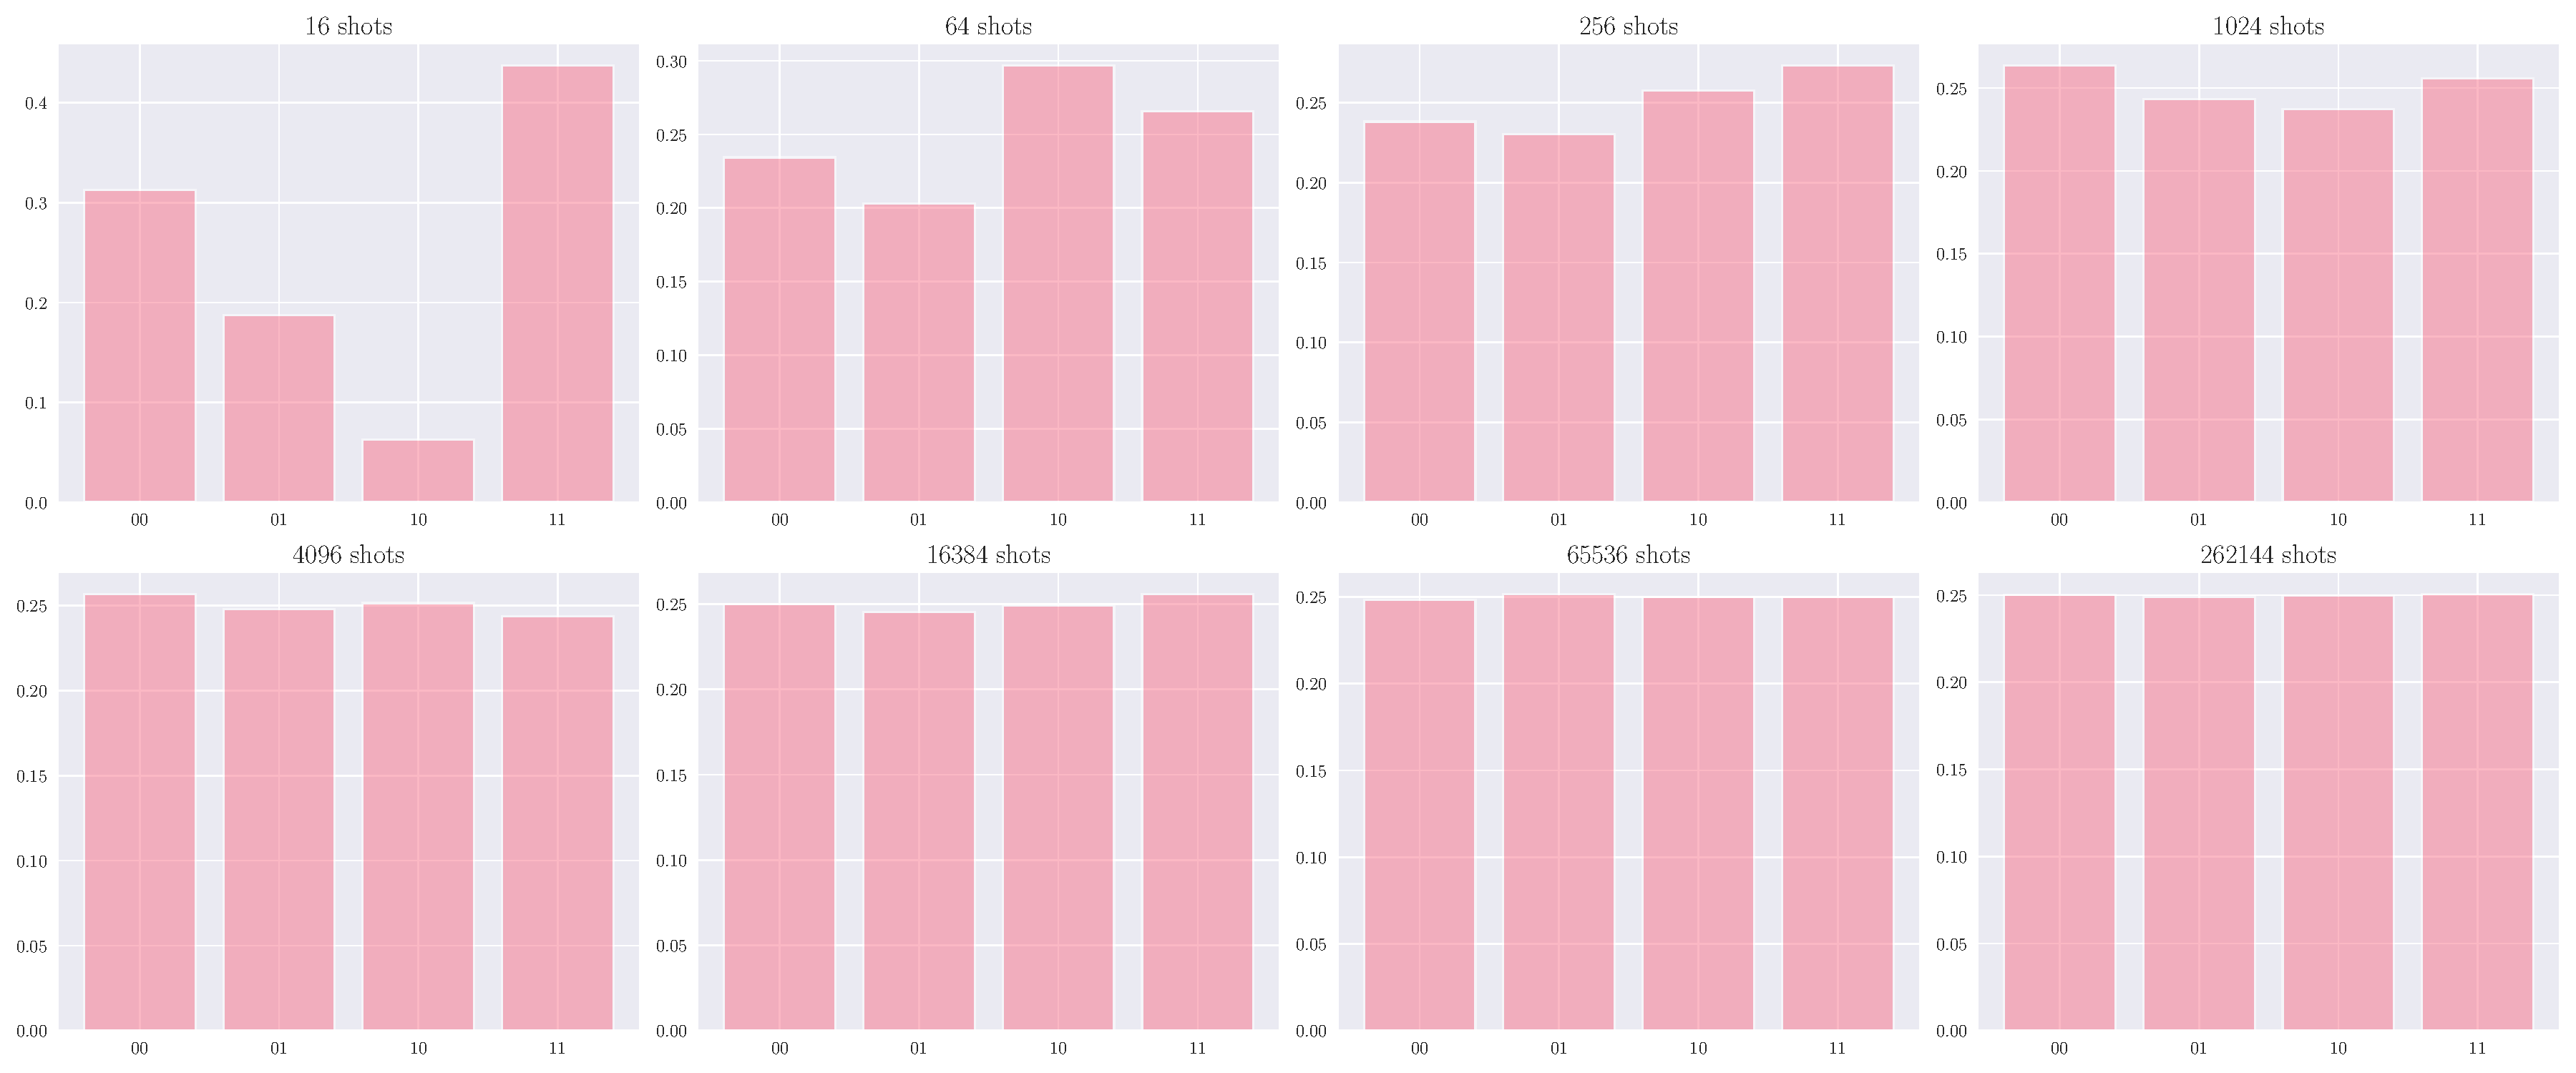
\includegraphics[width=\linewidth]{image/measurements_histogram.pdf}
	\caption{Histograms of classically simulated measurement results for state $\ket{\psi} $ with different number of shots. The horizontal axis labels the states being measured and the vertical axis shows the probability for measuring the corresponding state.}
	\label{fig:meas_result}
\end{figure}


\begin{figure}[ht]
	\centering
	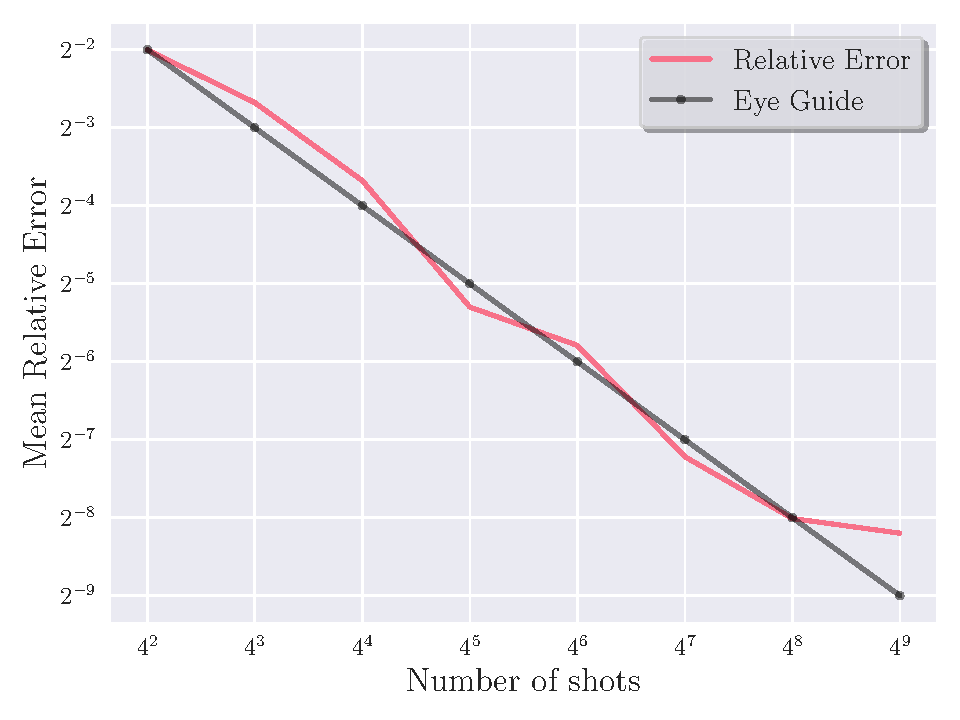
\includegraphics[width=0.8\linewidth]{image/mean_rel_error.pdf}
	\caption{Mean relative error for each shot. The red line is the result of a numerical simulation using the \texttt{Quanthon} library and the grey line is an eye guide with $ y = 1/\sqrt{x} $.}
	\label{fig:mean_rel_err}
\end{figure}

Figures~\ref{fig:meas_result} and ~\ref{fig:mean_rel_err} demonstrate the relationship between the error and the number of shots we see that the results agree quite well with the theoretical result: $ N \propto \mathcal{O}(\frac{1}{ \epsilon^2 }) $. In fact, from Figure~\ref{fig:mean_rel_err} we can estimate errors from measurements with $ \epsilon \propto \sqrt{\frac{1}{N}} $. Later we will show that the error from shot noise is the limiting factor for the accuracy of algorithms. 


\subsection{Gate}
\label{sub:gate}
The \texttt{Qubits} class contains common predefined gates as in Subsection~\ref{sub:qubits}.
To construct a custom gate, which can be parameterised, specify the name, the number of qubits being acted on and the matrix representation of the gate or a function which takes in parameters and generates the gate matrix. The matrix must be unitary according to Definition~\ref{def:unitary}. \\
Below is an example of how to construct an \texttt{Rz} gate for a two-qubit circuit.
\begin{mycode}
import numpy as np
from Quanthon.base import Gate
from Quanthon.utils import make_op_mat

def Rz(theta, n, i):
	"""
        Args: 
            theta: float, the angle of rotation in radians,
            n: int, the number of qubits in the system,
            i: int, the index to apply the gate to.
        
        Returns:
            mat: the matrix representing the rotation of qubit i by theta about the z-axis.
	"""
    
    rz = np.cos(theta/2)*np.eye(2) - 1j*np.sin(theta/2)*np.array([[0,1],[1,0]])
    mat = make_op_mat(rz, i) # this expands the matrix to the size of the full system
    return mat

n = 2
i = 0
# non-parameterised
theta = 0.5 * np.pi
mat = Rz(theta, n, i)
rz_gate = Gate("Rz", mat, n)

# Parameterised
rz_gate_param = Gate("Rz", lambda theta: Rz(theta,i,n), n, is_parametrised=True)
\end{mycode}

To use the custom gate, 
\begin{mycode}
	q = qubits(2)
	# apply the non-parameterised Rz gate
	q.circuit.append(rz_gate) # append the gate here without any parameter 
	q.run()

	# or the parameterised gate
	q.state = rz_gate_param.act(q.state, 0.5 * np.pi)
	
\end{mycode}
Note that custom gates do not currently support drawing.


\section{Expectation Value}
\label{sec:expectation}
The expectation value of an operator $ A $ is given as 
\[ \braket{\psi|A|\psi}. \]
In a real quantum computer, this value must be estimated through repeated measurements of the state of the qubits on different basis. Since the Pauli matrices together with the identity operator $ I $ form a basis for the $2 \times 2$ matrices ( $\mathcal{M}_{2\times 2}$), any operator in this space can be written in terms of a linear combination of these operators using methods given in Appendix~\ref{appsec:pauli_basis}.

Let $ P $ be a Pauli string, then the expectation value of $ P $ is given by
\begin{equation}
	\label{eq:expectation}
	\braket{\psi|P|\psi} = \braket{\psi|U^{\dagger}ZU|\psi}.
\end{equation}

One must find a unitary operator $ U $ such that $ U^{\dagger}ZU $ is equal to the basis we are trying to measure in the one-qubit case, and $ ZI\ldots I $ in the multiple-qubit case. When the unitary transformation $ U $ is applied to the circuit of which we want to measure the expectation value, the eigenvalues are preserved and the expectation value can be calculated in the new basis.

\subsection{Single Qubit}
\label{sub:single_qubit}
In general, the one qubit Hamiltonian can be written as 
\begin{equation}
	\label{eq:1qubit_hamiltonian}
	H = aI + bX + cY + dZ, \quad a,b,c,d \in \mathbb{C}. 
\end{equation}

Given the following relations relating the Pauli $ X $ and $ Y $ operator with the Pauli $ Z $,
\begin{align}
	\label{eq:basis-rotation}
	X = HZH, \\
	Y = -S^{\dagger}HZHS.
\end{align}

Then the expectation value is 
\begin{align}
	\braket{\psi|H|\psi} &= a\braket{\psi|I|\psi} + b \braket{\psi|X|\psi} + c \braket{\psi|Y|\psi} + d \braket{\psi|Z|\psi} \\
			     &= a \underbrace{\braket{\psi|\psi}}_{1} + b \braket{\psi|HZH|\psi} + c \braket{\psi|HS^{\dagger}ZSH|\psi} + d \braket{\psi|Z|\psi}.
\end{align}

The \texttt{expectation} function estimates the expectation values of a qubit Hamiltonian.

In the case of a single qubit, to rotate the computation basis to another Pauli basis, we simply apply the $H$ gate for when there is an $ X $ in the Hamiltonian, and $ S^\dagger$ gate followed by an $ H $ gate when there is a $ Y $-gate.

\begin{figure}[ht]
	\centering
	\begin{quantikz}
		  & \gate{U} & \gate{H}  &\qw\\
	\end{quantikz}
	\caption{The single qubit circuit which rotates a state to be measured in the $ X $ basis.}
	\label{fig:rotate-to-X-circuit}
\end{figure}

\subsection{Multiple Qubits}
\label{sub:multiple_qubits}
The computation basis is the Pauli $ Z\underbrace{I \ldots I}_{n-1}$ basis for an $ n $-qubit quantum circuit. 
When there is more than one qubit in the system if the operator contains only one non-identity operator on the first qubit, then a similar strategy applies --- apply the \texttt{H}-gate or the \texttt{Sdag}-gate followed by \texttt{H} gate on the first qubit. 

In the case where the Pauli string contains more than non-identity, for example, $ZI$ contains only one non-identity operator and $ZZ$ contains two, the \texttt{CNOT} gate must be applied to such qubits to disentangle them. Consider the smallest non-trivial case, the Pauli string $ ZZ $, the unitary transform which rotates the $ ZZ $ basis to the $ ZI $ basis is the $ CNOT_{10} $ gate,
\[
CNOT(1,0) =
\begin{bmatrix} 
1 & 0 & 0 & 0 \\
0 & 0 & 0 & 1 \\
0 & 0 & 1 & 0 \\
0 & 1 & 0 & 0 \\
\end{bmatrix} = CNOT(1,0)^{\dagger},  \] 
and
\begin{align}
	CNOT(1,0)(ZZ)CNOT(1,0) &= 
\begin{bmatrix} 
1 & 0 & 0 & 0 \\
0 & 0 & 0 & 1 \\
0 & 0 & 1 & 0 \\
0 & 1 & 0 & 0 \\ 
\end{bmatrix} 
\begin{bmatrix} 
1 & 0 & 0 & 0 \\
0 & -1 & 0 & 0 \\
0 & 0 & -1 & 0 \\
0 & 0 & 0 & 1 \\
\end{bmatrix} 
\begin{bmatrix}
1 & 0 & 0 & 0 \\
0 & 0 & 0 & 1 \\
0 & 0 & 1 & 0 \\
0 & 1 & 0 & 0 \\
\end{bmatrix} \\
&= 
\begin{bmatrix}
1 & 0 & 0 & 0 \\
0 & 1 & 0 & 0 \\
0 & 0 & -1 & 0 \\
0 & 0 & 0 & -1 \\
\end{bmatrix} = ZI.
\end{align}


\begin{figure}[ht]
	\centering
	\begin{quantikz}
		\lstick{$\ket{q_1}$} &\gate[2]{U} & \ctrl{1} & \qw \\
		\lstick{$\ket{q_2}$} & \qw & \targ{} & \qw
	\end{quantikz}
	\caption{The circuit to rotate the qubits into the $ ZZ $ basis.}
	\label{fig:disentangle-ZZ}
\end{figure}
In cases where the non-identity gates are not in the first positions, a series of SWAP gates are used to swap the state of the qubits with neighbouring qubits,

\begin{align}
	\label{eq:swap}
	SWAP(0,1)(IZ)SWAP(0,1) &=  
\begin{bmatrix}
1 & 0 & 0 & 0 \\
0 & 0 & 1 & 0 \\
0 & 1 & 0 & 0 \\
0 & 0 & 0 & 1 \\
\end{bmatrix}
\begin{bmatrix}
1 & 0 & 0 & 0 \\
0 & -1 & 0 & 0 \\
0 & 0 & 1 & 0 \\
0 & 0 & 0 & -1 \\
\end{bmatrix}
\begin{bmatrix}
1 & 0 & 0 & 0 \\
0 & 0 & 1 & 0 \\
0 & 1 & 0 & 0 \\
0 & 0 & 0 & 1 \\
\end{bmatrix} \\
&=
\begin{bmatrix}
1 & 0 & 0 & 0 \\
0 & 1 & 0 & 0 \\
0 & 0 & -1 & 0 \\
0 & 0 & 0 & -1 \\
\end{bmatrix} = ZI.
\end{align}
\begin{figure}[ht]
	\centering
	\begin{quantikz}
		\lstick{$\ket{q_1}$} &\gate[2]{U} & \swap{1} & \qw \\
		\lstick{$\ket{q_2}$} & \qw & \targX{} & \qw
	\end{quantikz}
	\caption{The circuit to rotate the qubits into the $ IZ $ basis.}
	\label{fig:swap-iz=zi}
\end{figure}

After the rotation, multiple measurements are taken to estimate the state of the qubits, since the eigenvalues are preserved under unitary transformations, the eigenvalues are the same as that of the $ ZI\ldots I $ state. For an $ n $ qubit system, the states $ \ket{0}  $ to $ \ket{2^{n-1}} $ have eigenvalues $ 1 $ and the rest have eigenvalues $ -1 $.

The \texttt{expectation} function handles all the procedures above for all combinations of Pauli strings.  The code snippet outlines the usage of the function.
\begin{mycode}
	from Quanthon import expectation
	q = Qubits(2)
	H = [("ZZ", 0.5), ("XI", 0.5)] # example Hamiltonian, must be given in [(operator, coefficient), ...] format.
	energy = cal_expectation(q, hamiltonian, n_shots=10000)
\end{mycode}


\section{Physics}
\label{sec:physics}
\subsection{Hamiltonian}
The \texttt{Hamiltonian} class stores the overlap integrals for one and two-body. These integrals need to have been calculated. In the case of molecular systems, these integrals can usually be obtained through quantum chemistry packages such as \texttt{PySCF}\cite{sun2018}.

\section{Mappers}
\label{sec:mappers}
\subsection{Jordan-Wigner}
\label{sub:jordan-wigner-mapper}
The Jordan-Wigner transformation maps the fermionic operators to qubit operators. The transformation is given in Section~\ref{sub:jw}.

The second quantised Hamiltonians are usually in the form of Equation~\eqref{eq:sq_hamiltonian}. We keep the integrals general without considering the symmetry of the system, i.e., $ p,q,r,s \in [0, N-1] $ for $ N $ basis functions for both the one- and two-body integrals. The mapping costs $ N $ qubits. The treatment depends on the value and order of the indices and whether it is a one- or two-body term.
\subsection{One-Body}
\label{sub:one-body}
The transformation of the one-body term $ a_{p}^{\dagger}a_q $using Equation~\eqref{eq:jw} is

\begin{equation}
	\label{eq:ob_jw}
a_{p}^{\dagger}a_q \\
				   = \left( \frac{1}{2} \left[ \bigotimes_{n=0}^{p-1} Z_n \right] \left( X_p - i Y_p \right)   \right) 
 \left( \frac{1}{2} \left[ \bigotimes_{n=0}^{q-1} Z_n \right] \left( X_q +i Y_q \right)   \right).
\end{equation}

Four relations are useful in the derivation of the later expressions:
\begin{align}
	\label{eq:useful_relations}
	(X-iY)Z &= -iY+X = (X-iY), \\
	Z(X-iY) &= iY - X = -(X-iY), \\
	(X+iY)Z &= -iY -X = -(X+iY),\\
	Z(X+iY) &= iY + X = (X+iY).
\end{align}

\subsubsection{For $p=q$}%
\label{ssub:p_equal_q}
When $p=q$, using properties of Pauli matrices in Appendix~\ref{app:pauli_properties}, the Jordan-Wigner transform of the term in Equation~\eqref{eq:ob_jw} becomes:
\begin{equation}
	\label{eq:p_equals_q}
	\begin{aligned}
		a_{p}^{\dagger}a_q &= a_{p}^{\dagger}a_p,  \\
				   &= \left( \frac{1}{2} \left[ \bigotimes_{n=0}^{p-1} Z_n \right] \left( X_p - i Y_p \right)   \right) 
 \left( \frac{1}{2} \left[ \bigotimes_{n=0}^{p-1} Z_n \right] \left( X_p +i Y_p \right)   \right), \\
				   &= \frac{1}{4} \left[ \bigotimes_{n=0}^{p-1} I_n \right] \left( X_p - i Y_p \right) \left( X_p + i Y_p \right),\\ 
	&= \frac{1}{4} \left[ \bigotimes_{n=0}^{p-1} I_n \right] \left( X_p^2 -iY_iX_i + iX_iY_i + Y_p^2 \right), \\
	&= \frac{1}{4} \left[ \bigotimes_{n=0}^{p-1} I_n \right] \left( 2I_p + 2iZ_p \right), \\
	&= \frac{1}{2} \left[ \bigotimes_{n=0}^{p-1} I_n \right] \left( I_p -Z_p \right),
	\end{aligned}
\end{equation}
which translates to two Pauli strings. In the case of $ N $ qubits $\underbrace{I\ldots I}_N$ and $\underbrace{I\ldots I}_{p}Z_p \underbrace{l \ldots I}_{N-p-1}$ respectively.


\subsubsection{For $p < q$}%
\label{ssub:p_lessthan_q}
In the case where $ p < q $, the $ Z $ operators on qubits on $ p $ and between $ p $ and $ q $ do not cancel out as in the $ p=q $ case, Equation~\eqref{eq:ob_jw} becomes:
\begin{equation}
	\label{eq:jw_p_lessthan_q}
	\begin{aligned}
		&= \frac{1}{4} \left[ \bigotimes_{n=0}^{p-1} I_n \right] \left( X_p - i Y_p \right)Z_p 
		\left[ \bigotimes_{n=p+1}^{q-1} Z_n \right]  \left( X_q + i Y_q \right) \\
		&= \frac{1}{4} \left[ \bigotimes_{n=0}^{p-1} I_n \right] \left( X_p - i Y_p \right) \left[ \bigotimes_{n=p+1}^{q-1} Z_n \right]  \left( X_q + i Y_q \right) \\
		&= \frac{1}{4} \left[ \bigotimes_{n=0}^{p-1} I_n \right] \left[ \bigotimes_{n=p+1}^{q-1} Z_n \right] \left( X_p - i Y_p \right)   \left( X_q + i Y_q \right) \\
		&= \frac{1}{4} \left[ \bigotimes_{n=0}^{p-1} I_n \right] \left[ \bigotimes_{n=p+1}^{q-1} Z_n \right] \left( X_pX_q - iY_pX_q + iX_pY_q + Y_pY_q \right). \\
	\end{aligned} 
\end{equation}
This translates to four Pauli strings:
\begin{align}
	\label{eq:p_lessthan_q}
	&\underbrace{I\ldots I}_{p}X_{{\color{blue}p}} \underbrace{Z\ldots Z}_{q-p-1}X_q \underbrace{I\ldots I}_{N-q} \\
	-i &\underbrace{I\ldots I}_{p}Y_{{\color{blue}p}} \underbrace{Z\ldots Z}_{q-p-1}X_q \underbrace{I\ldots I}_{N-q} \\
	i &\underbrace{I\ldots I}_{p}X_{{\color{blue}p}} \underbrace{Z\ldots Z}_{q-p-1}Y_q \underbrace{I\ldots I}_{N-q} \\
	  &\underbrace{I\ldots I}_{p}Y_{{\color{blue}p}} \underbrace{Z\ldots Z}_{q-p-1}Y_q \underbrace{I\ldots I}_{N-q}.
\end{align}

\subsubsection{For $p > q$}%
\label{ssub:p_greaterthan_q}

The equation is the same but with $ p $ and $ q $ swapped. The Pauli strings are also the same but since now $ p > q $, the operator with index $ q $ is on the left-hand side. 
\begin{align}
	\label{eq:p_greaterthan_q}
	&\underbrace{I\ldots I}_{p}X_{{\color{red}q}} \underbrace{Z\ldots Z}_{p-q-1}X_p \underbrace{I\ldots I}_{N-q} \\
	-i &\underbrace{I\ldots I}_{p}X_{{\color{red} q}} \underbrace{Z\ldots Z}_{p-q-1}Y_p \underbrace{I\ldots I}_{N-q} \\
	i &\underbrace{I\ldots I}_{p}Y_{{\color{red} q}} \underbrace{Z\ldots Z}_{p-q-1}X_p \underbrace{I\ldots I}_{N-q} \\
	  &\underbrace{I\ldots I}_{p}Y_{{\color{red} q}} \underbrace{Z\ldots Z}_{p-q-1}Y_p \underbrace{I\ldots I}_{N-q}.
\end{align}

\subsection{Two-Body}
\label{sub:two-body}
The two-body term $ a_{p}^{\dagger}a_{q}^{\dagger}a_ra_s $ is more complicated. The general Jordan-Wigner transform is.
\begin{equation}
	\label{eq:tb_jw}
	\begin{aligned}
		a_{p}^{\dagger}a_{q}^{\dagger}a_ra_s = 
		& \left( \frac{1}{2} \left[ \bigotimes_{n=0}^{p-1} Z_n \right] \left( X_p - i Y_p \right)   \right) 
		\left( \frac{1}{2} \left[ \bigotimes_{n=0}^{q-1} Z_n \right] \left( X_q - i Y_q \right)   \right) \\
		& \left( \frac{1}{2} \left[ \bigotimes_{n=0}^{r-1} Z_n \right] \left( X_r + i Y_r \right)   \right) 
	 \left( \frac{1}{2} \left[ \bigotimes_{n=0}^{s-1} Z_n \right] \left( X_s +i Y_s \right)   \right).\\
	\end{aligned}
\end{equation}
If the outer indices are not greater or less than the inner indices, the term will be different by a factor of $ -1 $ due to the creation operators being on the right-hand side, i.e. $ p > q \wedge r > s $ or $ p < q \wedge r < s$. \\
The results of the transformation depend on the values of the indices $ p,q,r,s $.

\subsubsection{For $p=q$ or $r=s$}%
\label{ssub:p_equals_q_or_r_equals_s}
According to the definition of the creation and annihilation operators, \[a_{p}^{\dagger}a_{p}^{\dagger} = 0, \] and \[ a_qa_q = 0.\] Therefore if the creation or the annihilation operators have the same indices, this term does not contribute.


\subsubsection{For $p=r \neq q=s$ or $p=s \neq q=r$}%
\label{ssub:two_pairs}
Since $p=r$ and $q=s$, all the $ Z $ operators cancel out since there are always an even number of $ Z $ operators on every qubit, then Equation~\eqref{eq:tb_jw} simplifies to:
\begin{equation}
	\label{eq:jw_p_equals_q_r_equals_s}
	\begin{aligned}
		a_{p}^{\dagger}a_{q}^{\dagger}a_ra_s &= a_{p}^{\dagger}a_{q}^{\dagger}a_pa_q \\
		&= \frac{1}{4} \left[ \bigotimes_{n=0}^{p-1} I_n \right] \left( I_p - Z_p \right)  \left[ \bigotimes_{n=p+1}^{q-1} I_n \right] \left( I_q - Z_q \right)\\
		&= \frac{1}{4} \left[ \bigotimes_{n=0}^{p-1} I_n \right]  \left[ \bigotimes_{n=p+1}^{q-1} I_n \right] \left( I_pI_q - Z_pI_q - I_pZ_q + Z_pZ_q \right).\\
	\end{aligned}
\end{equation}

\subsubsection{For $p \neq q \neq r \neq s$ }%
\label{ssub:4_unique}
In the case where all the indices are unique, we first sort the indices so that $ a<b<c<d \equiv \texttt{sorted(p,q,r,s)}$, which gives

\begin{equation}
	\label{eq:jw_4_unique}
	\begin{aligned}
		a_{p}^{\dagger}a_{q}^{\dagger}a_ra_s &= \frac{1}{16} \left[ \bigotimes_{n=0}^{a-1} I_n \right] \left( X_a \pm i Y_a \right)Z_a 
		\left[ \bigotimes_{n=a+1}^{b-1} Z_n \right]  \left( X_b \pm i Y_b \right) \\
		&   \left[ \bigotimes_{n=b+1}^{c-1} I_n \right] \left( X_c \pm i Y_c \right)Z_c  \left[ \bigotimes_{n=c+1}^{d-1} Z_n \right] \left( X_d \pm i Y_d \right),
	\end{aligned}
\end{equation}
where the $ \pm $ depends on whether the associated operator is a creation or annihilation operator. These would result in $ 16 $ unique Pauli strings of products of the $ (X \pm iY) $ terms.

\subsubsection{For $ 3 $ unique indices}%
\label{ssub:3_unique}
The expression for the case where there are $ 3 $ unique indices changes depending on which index is repeated. Since the two creation and annihilation operators do not have the same index as discussed in Subsection~\ref{sub:jordan-wigner-mapper}, the three qubits that are being acted on must contain a creation operator, an annihilation operator and a product of both, which is given by $(X-iY)(X+iY) = (I-Z)$ following similar derivation of Equation~\ref{eq:p_equals_q}.

\subsubsection{Example Code}%
\label{ssub:jw-example}
The Jordan-Wigner transformation can be done by calling the \texttt{jordan\_wigner} function, which takes in an instance of \texttt{Hamiltonian} and handles all the above cases then returns a list of Pauli strings with coefficients. 
\newpage
\begin{mycode}	
	from Quanthon import Hamiltonian, jordan_wigner

	# Generate random one- and two-body integrals
	one_body = np.random.rand(n,n) + 1j*np.random.rand(n,n)
    	one_body = one_body + one_body.conj().T

    	two_body = np.random.rand(n,n,n,n) + 1j*np.random.rand(n,n,n,n)
    	two_body = two_body + two_body.conj().T

	hamiltonian = Hamiltonian(one_body, two_body)

	qubit_hamiltonian = jordan_wigner(hamiltonian)
\end{mycode}

\subsection{Pauli Decomposition}
\label{sub:pauli-decomposition-mapper}
In the case where a Hamiltonian is already written in matrix representation, Pauli decomposition as in Equation~\eqref{eq:pauli-decomp} can be used for a mapping which scales with $\lceil \log_2(N) \rceil$ for an $ N\times N $ matrix. The \texttt{pauli\_decomposition} function takes in a matrix and returns a list of Pauli strings with coefficients. In the case where the Hamiltonian is not of size $2^n \times 2^n$, $0$'s are padded to all non-diagonal entries and a number larger than the ground state energy such as $999$, to the diagonal entries to make it of that shape. $ 999 $ is an arbitrarily large number so that the additional rows and columns do not affect the ground state energy.
\begin{mycode}
	from Quanthon import pauli_decomposition
	matrix = np.random.rand(4,4) + 1j*np.random.rand(4,4)
	matrix = matrix + matrix.conj().T
	pauli_strings = pauli_decomposition(matrix)
\end{mycode}

\section{Exponentials}
\label{sec:exp}
Taking the exponential of a Pauli string is an inevitable and common step in quantum computing. Being able to take the exponential of a Pauli string allows us to implement, for example, the ADAPT-VQE. We have implemented two different algorithms for creating circuits for the exponentials that are both exact and equivalent mathematically, the first is the so-called Staircase algorithm and the second is the Inverted Staircase algorithm~\cite{Mansky2023}.
\subsection{Staircase Algorithm}%
\label{ssub:StaircaseAlgorithm}
The Staircase algorithm is an algorithm that decomposes the exponential into a rotation about the $ Z $ axis and CNOT gates. We will show that this is equivalent to the exponential itself. 
Given an exponential of a Pauli string $ e^{-i\theta P} $, where $ \theta $ is a real parameter. The exponential of a Pauli operator $ \sigma_j $  for the one qubit case can be written as
\begin{align}
	\label{eq:ExpPauli}
	 e^{-i\theta \sigma_j} &= \cos(\theta \sigma_j) + i \sin(\theta \sigma_j) \\
	&= \sum_k \left(   (-1)^k \frac{(\theta \sigma_j)^{2k}}{(2k)!}  \right) +  i \sum_k \left((-1)^k \frac{(\theta \sigma_j)^{2k+1}}{(2k+1)!} \right)\\
		&= \cos(\theta)I - i\sin(\theta)\sigma_j,
\end{align}
since
\begin{equation}
	\label{eq:paulisquareisidentity}
	\sigma_j^{2k} = I  \text{ and }  \sigma_j^{2k+1} = \sigma_j,  \quad \text{ for } k \in \mathbb{N}.
\end{equation}
This, incidentally, is the rotation gate $ R_{\sigma_j}(2\theta)$.
This is true for Pauli strings acting on any number of qubits since the matrix product acts on only one of the subspaces and operators acting on different qubits commute, hence Equation~\eqref{eq:paulisquareisidentity} holds. In general, for any Pauli string $ P $ 
\begin{equation}
	\label{eq:multiqubitrotation}
	e^{-i\theta P} = \cos(\theta)I - i\sin(\theta)P.
\end{equation}
Hence, the exponential of a Pauli string is a rotation about the axis specified by the Pauli string in the $ N $ dimensional hypersphere, where $ N $ is the number of qubits, analogous to the Bloch sphere for a single qubit. However, performing a multi-qubit rotation is not as straightforward as the single-qubit case. Using similar methods to the rotation of basis, we could find $ U $ such that
\[ U(e^{-i\theta P})U^{\dagger} = e^{-i\theta Z^{\otimes N}}. \] 
The results are similar to Equation~\eqref{eq:basis-rotation} --- for every $ X $ in the Pauli string, \[ U=U^{\dagger}=H. \] 
Here we chose for $ Y $ a slightly different unitary operator \[ U=Y_L \equiv R_z\left( \frac{-\pi}{2} \right)H, \] and \[ U^{\dagger} = Y_R \equiv = H Rz(\frac{-\pi}{2}). \]
Finally, to covert a rotation about the $ Z^{\otimes k} $ to single qubit rotations $ R_z $ we again choose $ U_2=\{\cnot(j,j+1)\}$ for $ j \in \{0, \ldots, N-2\} $ so that

\[ U\left( e^{-i\theta Z^{\otimes N}} \right)U^{\dagger} = e^{-i\theta I \ldots I Z}.\] 
In the case where there are non-connected operators in the Pauli string, the SWAP gate is used instead of the CNOT gate.
For example, if the Pauli string $ P = XYZI $, the unitary transformation $ U $ would be \[ H \cnot(0,1) \otimes Y_L \cnot(1,2) \otimes \swp(2,3) \otimes I.\] In quantum circuit notation, this is
\begin{figure}[ht]
	\centering
	\begin{quantikz}
		\lstick{$\ket{q_1}$} &\gate{H} & \ctrl{1}& \qw & \qw & \qw & \qw & \qw &\ctrl{1} & \gate{H} & \qw \\
		\lstick{$\ket{q_2}$} & \gate{Y_L} & \targ{} & \ctrl{1} & \qw & \qw &\qw & \ctrl{1} & \targ{} & \gate{Y_R} & \qw \\
		\lstick{$\ket{q_3}$} & \qw & \qw & \targ{} & \swap{1} & \qw & \swap{1} &\targ{} & \qw &\qw &\qw\\
		\lstick{$\ket{q_4}$} & \qw & \qw & \qw & \targX{} & \gate{R_z(2\theta)} & \targX{} & \qw &\qw &\qw &\qw
	\end{quantikz}
	\caption{The circuit to exponentiate $ -i\theta XYZI $ with the Staircase algorithm.}
	\label{fig:rotate-to-XYIZ}
\end{figure}

The structure of the circuit looks like a staircase made of CNOT gates.

\subsection{Inverted Staircase Algorithm}
\label{sub:invertedstaircase}
The inverted staircase algorithm was proposed to reduce the number of single-qubit gates, using $ R_x $ as the single qubit rotation instead of the $ R_z $ gate, as well the equivalent circuit shown in Figure~\ref{fig:hcnothinvertedcnot}, 
\begin{figure}[ht]
	\centering
	\begin{quantikz}
		\lstick{$\ket{q_1}$} &\gate{H} & \targ{} & \gate{H} & \qw \\
		\lstick{$\ket{q_2}$} & \gate{H} & \ctrl{-1} & \gate{H} & \qw 
	\end{quantikz}
	$\quad \equiv \quad $
	\begin{quantikz}
		&\ctrl{1}& \qw & \\
		&\targ{} & \qw &
	\end{quantikz}
	\caption{Equivalent circuit used in the Inverted Staircase Staircase.}
	\label{fig:hcnothinvertedcnot}
\end{figure}
In the Inverted Staircase algorithm, we try to find a mapping $ U $ such that 
\[ Ue^{-i\theta P}U^{\dagger} = e^{-i\theta I\ldots X}.\] 
Then for every $ Z $ in the Pauli string, apply a $ H $ gate on both the left and the right side of the CNOT (or SWAP) staircase, and for every $ Y $  apply a $ R_z(\frac{\pi}{2}) $ gate since
\[ R_z\left(\frac{\pi}{2}\right)X R_z\left(-\frac{\pi}{2}\right) = Y.\] 
Using the same example Pauli string $ XYIZ $ as in the Staircase algorithm example, the circuit with Inverted Staircase algorithm is shown in Figure~\ref{fig:rotate-to-XYIZ-inverted}.
\begin{figure}[ht]
	\centering
	\begin{quantikz}
		\lstick{$\ket{q_1}$} & \qw & \targ{}& \qw & \qw & \qw & \qw & \qw &\targ{} & \qw & \qw \\
		\lstick{$\ket{q_2}$} & \gate{R_z \left(\frac{\pi}{2}\right)} & \ctrl{-1} & \targ{} & \qw & \qw &\qw & \targ{} & \ctrl{-1} & \gate{R_z \left( \frac{\pi}{2} \right) 	} & \qw \\
		\lstick{$\ket{q_3}$} & \qw & \qw & \ctrl{-1} & \swap{1} & \qw & \swap{1} &\ctrl{-1} & \qw &\qw &\qw\\
		\lstick{$\ket{q_4}$} & \qw & \qw & \qw & \targX{} & \gate{R_x(2\theta)} & \targX{} & \qw &\qw &\qw &\qw
	\end{quantikz}
	\caption{The circuit to exponentiate $ -i\theta XYIZ $ using the Inverted Staircase algorithm.}
	\label{fig:rotate-to-XYIZ-inverted}
\end{figure}

Comparing Figure~\ref{fig:rotate-to-XYIZ} and Figure~\ref{fig:rotate-to-XYIZ-inverted}, the Inverted Staircase algorithm has fewer single qubit gates (3) than the Staircase algorithm (7). Being able to reduce the number of single-qubit gates is important in the NISQ era. Table \ref{tab:exponential-comparison} shows the comparison of the two algorithms for different Pauli strings.
\begin{table}[ht]
	\centering
	\begin{tabular}{c||c c c}
		\toprule
		Pauli String & Length & Number of SQG (Staircase) & Number of SQG (Inverted Staircase) \\
		\midrule
		$XX$ & $2$ & $7$ & $3$ \\
		$YY$ & $2$ & $11$ & $7$ \\
		$ZZ$ & $2$ & $3$ & $7$ \\
		$XYXY$ & $4$ & $19$ & $11$ \\
		$XYIZ$ & $4$ & $13$ & $11$ \\
		$IXIZ$ & $4$ & $9$ & $9$ \\
		$XYZXYZ$ & $6$ & $23$ & $19$ \\
		\midrule
		\textbf{Total} & & $85$ & $67$ \\
	\bottomrule
	\end{tabular}
	\caption{Comparison of the number of single-qubit gates for the Staircase and Inverted Staircase algorithms.}
	\label{tab:exponential-comparison}
\end{table}
It is not difficult to see from Table~\ref{tab:exponential-comparison} that if we ignore the one qubit rotation in the centre for both algorithms, the Inverted Staircase algorithm is more efficient in terms of the number of single-qubit gates by having the opposite number of gates for $ X $ and $ Z $ operators compared to the Staircase algorithm, but half as many for $ Y $ operators.

\subsection{Example Code}%
\label{sub:exp-example}
The function \texttt{exponential\_pauli} takes in a \texttt{Qubits} object, the Pauli string to exponentiate and the parameter $ \theta $ for the keyword \texttt{coefficient}. It appends the gates using either the staircase or the inverted staircase algorithms to the circuit. Users can specify the algorithm by passing in either ``staircase'' or ``inverted\_staircase'' to the keyword \texttt{method}. The code snippet below shows how to use the function. Note that this function currently only supports two or more qubits, in the one qubit case, a normal rotation gate can be used.
\begin{mycode}
	from Quanthon import exponential_pauli
	q = Qubits(4)
	# the resulting circuit will be appended onto the circuit of the qubits object
	exponential_pauli(q, "XYIZ", np.pi/2, method="inverted_staircase")
\end{mycode}

\section{Ansatz}
\label{sec:ansatz}
The \texttt{Ansatz} module contains different ansatz which are used together with VQEs and potentially other variational algorithms. \texttt{Ansatz} is the based class for all fixed-form ansatz, such as the \texttt{HardwareEfficientAnsatz}, and \texttt{QubitAdaptAnsatz} is an ansatz which evolves every iteration.

\subsection{Hardware Efficient Ansatz}
\label{sub:hea}
The Hardware Efficient Ansatz is popular since it is easy to implement on a quantum computer. Consists of single qubit rotation gates and linear entanglement gates with CNOT, construct a circuit similar to the one shown in Figure~\ref{fig:4hw}. The \texttt{HardwareEfficientAnsatz} class contains methods \texttt{create\_circuit} and \texttt{run} which are called when passed as an ansatz to the VQE class.
\begin{mycode}
	from Quanthon import HardwareEfficientAnsatz
	ansatz = HardwareEfficientAnsatz(n_qubits=2, rep=2)
\end{mycode}

\subsection{RyAnsatz}
\label{sub:ryansatz}
The RyAnsatz is also a type of hardware efficient ansatz except with only $ R_y $ gates instead of both $ R_x $ and $ R_y $. The \texttt{RyAnsatz} class contains the same methods as the \texttt{HardwareEfficientAnsatz} class and is used in the same way. Note that the number of parameters is $ n_{\text{qubits}} $ per rep instead of $ 2n_{\text{qubits}} $ as in the \texttt{HardwareEfficientAnsatz} class. The \texttt{RyAnsatz} typically achieves the same accuracy as the \texttt{HardwareEfficientAnsatz} but with only half as many parameters, and it is therefore more recommended for NISQ devices.


\subsection{QubitAdaptAnsatz}
\label{sub:qubit-adapt-ansatz}
QubitAdaptAnsatz is an ansatz which evolves with every iteration and it is used together with the \texttt{AdaptVQE} in Subsection~\ref{sub:implementation-adapt-vqe}.

The \texttt{QubitAdaptAnsatz} class takes in the number of qubits and a pool, which could either be ``V'', ``Vx'' or ``G'', or a custom pool given as a list of Pauli strings, default to ``V''. The $V$ and $G$ pool are given in Section~\ref{sub:qubit_adapt_vqe}, where ``Vx'' has the same structure as ``V'' but all the $ Y $ gates are replaced by $ X $ gates. 

The \texttt{append\_op} method is called in the \texttt{AdaptVQE} class to append the parameterised version of the exponential of the selected operator. The \texttt{QubitAdaptAnsatz} class also contains a \texttt{Qubits} object to which the circuit is appended. 

There are also two different methods for running the circuit, \texttt{run} and \texttt{run\_without\_update}, the former updates the state and the latter returns the results while retaining the original state. These options are important for the AdaptVQE algorithm.

An initial state can also be passed in during initialisation, if not, the \texttt{Qubits} object will be initialised to the $ \frac{1}{\sqrt{2^{N-1}}} (\ket{0\ldots 0} + \ldots + \ket{1\ldots 1}  $ state. The code snippet below shows how to use the \texttt{QubitAdaptAnsatz} class.
\begin{mycode}
	from Quanthon import QubitAdaptAnsatz
	ansatz = QubitAdaptAnsatz(n_qubits=2, pool="G")
\end{mycode}
\section{Algorithms}
\label{sec:algo}
This section explains the structure for \texttt{algorithms.py}, including \texttt{VQE} and \texttt{ADAPT-VQE}. 

\subsection{VQE}
\label{sub:algo-vqe}
The \texttt{VQE} class has used an implementation of the Variational Quantum Eigensolver which can be used with any fixed-form ansatz,  in this example we will use the \texttt{qubit\_hamiltonian} and \texttt{HardwareEfficientAnsatz} created in code blocks in Subsection~\ref{sub:hea} and Sub-subsection~\ref{ssub:jw-example}.

The \texttt{\_\_init\_\_} method takes in the ansatz and the initial parameters for the ansatz. An \texttt{optimiser} can be passed in as an argument, if so, the optimiser must take the same arguments as \texttt{scipy.optimize.minimize}. If not, it defaults to \texttt{scipy.optimize.minimize}. 

The \texttt{minimise\_eigenvalue} method takes in the Hamiltonian and the number of shots for the simulation. The code snippet below shows how to use the \texttt{VQE} class.
\begin{mycode}
	from Quanthon import VQE
	# initialise the parameters with random values
	rng = np.random.default_rng(9999)
	init_points = rng.random(ansatz.n_params) * 2 * np.pi - np.pi

	vqe = VQE(ansatz, init_points)
	results = vqe.minimise_eigenvalue(qubit_hamiltonian, num_shots=10000)

\end{mycode}

\subsection{AdaptVQE}
\label{sub:implementation-adapt-vqe}
The \texttt{AdaptVQE} class is an implementation of the Adaptive Variational Quantum Eigensolver. To initialise an \texttt{AdaptVQE} object, 

\begin{itemize}
	\item an instance of the \texttt{QubitAdaptAnsatz} must be passed in;
	\item an optional boolean parameter \texttt{estimate\_energy} may be passed in. If set to \texttt{True}, the energy is estimated using the \texttt{cal\_expectation} function from \texttt{expectation}, otherwise the analytical values of $ \braket{\psi|H|\psi} $ are calculated. Default is \texttt{True};
	\item an \texttt{optimiser} may also be passed in, if so, the optimiser must take the same arguments as \texttt{scipy.optimize.minimize}. It is default to \texttt{scipy.optimize.minimize};
	\item upon initialisation, a variable $ \texttt{obj\_call}$ is initialise
\end{itemize}

The \texttt{run\_adapt\_circuit} method is called to start the ADAPT circuit, which takes in a qubit Hamiltonian in terms of Pauli operators and their coefficients. Optional parameters include 
\begin{itemize}
	\item \texttt{num\_shots} for the number of shots in every measurement, 
	\item \texttt{grad\_eps} default is $10^{-3}$. The gradient threshold below which the algorithms stops and is considered converged, 
	\item \texttt{method} the classical optimisation method to use,
	\item \texttt{max\_iter} the maximum number of ADAPT iterations before the algorithm stops even if convergence gradient is not reached,
	\item \texttt{decompose\_exp}, if set to \texttt{True}, the exponential of the Pauli strings are decomposed into available gates, if \texttt{False} \texttt{scipy.linalg.expm} is used to calculate the exponential instead, default is \texttt{True}.
	\item \texttt{decompose\_method} the method to use for decomposing the exponential, either ``staircase'' or ``inverted staircase'', default is ``staircase''. 
	\item \texttt{print\_log}, default is \texttt{False}, if set to \texttt{True}, the energy, operator appended and the gradient at every iteration is printed.
	\item \texttt{opt\_log}, default is \texttt{False}, sets the value of ``disp'' in the \texttt{scipy.optimize.minimize} method. Returns the optimisation information.

\end{itemize}
When the \texttt{run\_adapt\_circuit} method is called, it calculates the gradient by calling the \texttt{gradient} method for every operator in the pool to select the operator with the largest gradient, then appends it to the circuit of the ansatz and finally calls the \texttt{minimise\_eigenvalue} method to minimise the \texttt{\_objective} function which is the energy of the system. If either the maximum iteration is reached or the gradient is below the threshold, the algorithm stops and returns the optimal parameters and the minimised energy.


The \texttt{AdaptVQE} class also contain an instance of an \texttt{AdaptHistory} object which stores the minimised energy and the operators appended at every ADAPT iteration. It can be accessed via the \texttt{hist} member.
The code snippet below demonstrates the usage of the \texttt{AdaptVQE} class.
\begin{mycode}
	from Quanthon import AdaptVQE
	# initialise the AdaptVQE object with the QubitAdaptAnsatz from the previous code block
	adapt_vqe = AdaptVQE(ansatz)
	energy = adapt_vqe.run_adapt_circuit(qubit_hamiltonian, 
					     num_shots=10000,
					     grad_eps=1e-6, 
					     method="COBYLA", 
					     max_iter=max_iter, 
					     decompose_exp=True,
					     decompose_method="inverted staircase")[1])
	# get a history of the energies at every iteration
	iteration_energy = adapt_vqe.hist.min_energies 
\end{mycode}

\subsubsection{AdaptHistory}
\label{ssub:adapt-history}
The \texttt{AdaptHistory} class stores the following information for every iteration:
\begin{itemize}
	\item \texttt{min\_energies} the minimised energy at every iteration,
	\item \texttt{operators\_appended} the operators appended at every iteration,
	\item \texttt{max\_grads} the maximum gradients for any operator in the ADAPT pool at every iteration.
\end{itemize}

\subsubsection{Optimisers}
\label{ssub:optimisers}
The classical optimisation is done using the \texttt{scipy.optimize.minimize}~\cite{scipy}. The ones we will be using in this project are:
\begin{itemize}
	\item \texttt{Powell}, the Powell method is a minimisation method which performs a series of one-dimensional minimisation along a set of directions to explore the parameter space efficiently until convergence is reached~\cite{powell1964}.
	\item \texttt{COBYLA}, Constrained Optimization BY Linear Approximation is another derivative-free ~\cite{powell1994}.
	\item \texttt{SLSQP}, Sequential Least Squares Programming is a gradient-based method~\cite{kraft1988}.
	\item \texttt{BFGS}, Broyden-Fletcher-Goldfarb-Shanno is a quasi-Newton method which approximates the Hessian matrix using the gradients of the objective function~\cite{bfgs}.
	\item \texttt{L-BFGS-B}, Limited-memory Broyden-Fletcher-Goldfarb-Shanno is a limited-memory version of the BFGS method which also allows bounds~\cite{byrd1995}.
	\item \texttt{Nelder-Mead}, the Nelder-Mead method is a direct search method which does not require the gradient of the objective function~\cite{Nelder1965}.
\end{itemize}

These methods include both gradient-based and gradient-free methods. We will later compare their performances in the results section.


\section{VQE Utils}
The \texttt{vqe\_utils.py} is not a module of Quanthon. However, it is how we conducted the quantum simulations later on and we will show it here as an example. It contains two essential functions which assist us in simulating the above system using the quantum computing library \texttt{Quanthon}. The \texttt{run\_hw} function uses one of the two native fixed form ansatz, the \texttt{HardwareEfficientAnsatz} or \texttt{RyAnsatz}. It takes in the following arguments
\begin{itemize}
    \item \texttt{h} : The qubit Hamiltonian of the system.
    \item \texttt{method} : The classical optimiser to use.
    \item \texttt{rep}: The number of repetitions of the ansatz. The default is 2.
    \item \texttt{estimate\_energy} : If \texttt{True} the energy is estimated using the \texttt{cal\_expectation} function, if \texttt{False} the energy is calculated exactly. The default is \texttt{True}.
    \item \texttt{n\_shots}: The number of shots used for measurements. The default is 10000.
    \item \texttt{ansatz\_type} : The type of ansatz to use, either \texttt{hw} or \texttt{ry}. The default is \texttt{hw}.
    \item \texttt{init\_state} : The initial state of the system. If \texttt{None} the initial state is the equal superposition state $ \ket{+^{\otimes n}} $. Default is \texttt{None}.
    \item \texttt{opt\_log} : If \texttt{True} the optimisation log is printed. Sets the values for ``disp'' in the optimiser. The default is \texttt{False}.
\end{itemize}
The function returns the energy of the system and the final state of the qubits.

The other function \texttt{run\_adapt} allows us to run the ADAPT-VQE with the \texttt{QubitAdaptAnsatz}. It takes in the following arguments.

\begin{itemize}
    \item \texttt{h} : The qubit Hamiltonian of the system.
    \item \texttt{max\_iter}: The maximum number of ADAPT iterations allowed. The default is 100.
    \item \texttt{pool} : The ADAPT operator pool. The default is ``V''.
	\item \texttt{num\_shots}: The number of shots used for measurements. The default is 10000.
	\item \texttt{method} : The classical optimiser to use. The default is \texttt{COBYLA}.
		\item \texttt{decompose\_exp}: If \texttt{True} the exponential of the Hamiltonian is decomposed into hardware friend gates, if not, \texttt{scipy.linalg.expm} is used. The default is \texttt{True}.
	\item \texttt{decompose\_method}: The method to use for the decomposition of the exponentials. The default is ``inverted staircase''.
	\item \texttt{init\_state} : The initial state of the system. If \texttt{None} the initial state is the equal superposition state $ \ket{+^{\otimes n}} $. Default is \texttt{None}.
	\item \texttt{print\_log} : If \texttt{True} the log of the ADAPT process is printed. The default is \texttt{False}.
	\item \texttt{opt\_log} : If \texttt{True} the optimisation log is printed. Sets the values for ``disp'' in the optimiser. The default is \texttt{False}.
    \end{itemize}


\chapter{Physical Systems}
\label{chap:physical_systems}

\section{Hydrogen Molecule}
\label{sec:hydrogen_molecule}
The hydrogen molecule, ($ H_2 $), is the smallest molecule in chemistry. It consists of two hydrogen atoms, each with one electron. In quantum chemistry, the hydrogen molecule is often used as a benchmark for quantum algorithms. Reproducing the results of using the VQE to find the ground state energy of the hydrogen molecule is almost a textbook task in quantum computing for electronic structures. The result can also be easily benchmarked against traditional quantum chemistry methods, such as Hartree-Fock~\cite{Coleman2015}. For \quanthon, it serves as an example of how to use the software to solve electronic structure problems. 

The non-relativistic Hamiltonian for a general molecule in second quantisation is given by
\begin{equation}
	\label{eq:hamiltonian}
	H = h_{nuc} + \sum_{pq} h_{pq} a_p^\dagger a_q + \frac{1}{2} \sum_{pqrs} h_{pqrs} a_p^\dagger a_q^\dagger a_s a_r,
\end{equation}
where $ h_{nuc} $ is the interaction between nuclei and electrons, and $ h_{pq} $ and $ h_{pqrs} $ are the one and two electron integrals respectively. 
\begin{equation}
	\label{eq:elctron_integrals}
\begin{aligned}
& h_{p q}=\int d \sigma \varphi_p^*(\sigma)\left(-\frac{\nabla_{\vec{r}}^2}{2}-\sum_i \frac{Z_i}{\left|\vec{R}_i-\vec{r}\right|}\right) \varphi_q(\sigma), \\
& h_{p q r s}=\int d \sigma_1 d \sigma_2 \frac{\varphi_p^*\left(\sigma_1\right) \varphi_q^*\left(\sigma_2\right) \varphi_s\left(\sigma_1\right) \varphi_r\left(\sigma_2\right)}{\left|\vec{r}_1-\vec{r}_2\right|}, \\
& h_{n u c}=\frac{1}{2} \sum_{i \neq j} \frac{Z_i Z_j}{\left|\vec{R}_i-\vec{R}_j\right|},
\end{aligned}
\end{equation}
where $ Z_i $ is the charge of the nuclei and $ \vec{R} $ and  $\vec{r} $ are the spatial coordinates of the nuclei and electrons respectively. The functions $ \varphi $ are the one electron functions, often called spin orbitals in quantum chemistry, and are usually obtained from methods such as the Hartree Fock~\cite{Romero2019}. Fortunately, for the hydrogen molecule and many other systems, these integrals have been pre-calculated and we will be able to obtain them by using packages such as PySCF~\cite{sun2018}.

We will use the minimal basis set, namely the STO-3G basis set, which consists of three Gaussian functions for each atomic orbital~\cite{hehre1969self}. The choice of the basis set is to minimise the number of qubits required to represent the system since it is the accuracy of our VQE algorithms that is our main concern rather than capturing all the physics of the system. 

In this basis, the values we obtain for the hydrogen molecule are in Table~\ref{tab:hij} and Table~\ref{tab:hijkl}. With molecule geometry of
\begin{equation}
	\begin{aligned}
		\vec{R}_1 &= (0,0,0), \\
		\vec{R}_2 &= (0,0,0.735),
	\end{aligned}
\end{equation}
in units of angstrom (Å).

\begin{table}[h]
    \centering
    \caption{One-electron integral values of the hydrogen molecule in the STO-3G basis set.}
    \label{tab:hij}

    \begin{tabular}{c c}
        \toprule
        Integral & Values \\
        \midrule
        $h_{00} = h_{11}$ & $-1.252477$ \\
        $h_{22} = h_{33}$ & $-0.47189601$ \\
        \bottomrule
    \end{tabular}
\end{table}

\begin{table}[h]
    \centering
    \caption{Two-electron integral values for the STO-3G basis set.}
    \label{tab:hijkl}

    \begin{tabular}{c c}
        \toprule
        Integral & Values \\
        \midrule
	$h_{0000} = h_{0220} = h_{2002} = h_{2222}$ & $0.33785508$ \\
	$h_{0011} = h_{0101} = h_{0231} = h_{0321} = h_{1010} = h_{1100} = h_{1230} = h_{1320}$ & $0.09046560$ \\
	$h_{2013} = h_{2103} = h_{2233} = h_{2323} = h_{3012} = h_{3102} = h_{3232} = h_{3322}$ & $0.09046560$ \\
        $h_{0110} = h_{0330} = h_{1001} = h_{1221} = h_{2332} = h_{3003} = h_{3223}$ & $0.33229087$ \\
        $h_{1111} = h_{1331} = h_{3113} = h_{3333}$ & $0.34928686$ \\
        \bottomrule
    \end{tabular}
\end{table}


With this information, we could now perform the Jordan-Wigner transform implemented in Subsection~\ref{sub:jordan-wigner-mapper}. The resulting qubit Hamiltonian is 
\[\sum_{i} C_i\mathcal{P}_i,\]
where $\mathcal{P}_i$ is a Pauli string and their corresponding coefficients are given in Table~\ref{tab:qubit-hamiltonian-h2}.
\begin{table}[h]
	\centering
	\caption{Qubit Hamiltonian after Jordan-Wigner transform.}
	\label{tab:qubit-hamiltonian-h2}


	\begin{tabular}{c c}
		\toprule
		\textbf{Pauli String} & \textbf{Coefficients} \\
		\midrule
		IIII & $-0.81054798$  \\ 
		IIIZ & $-0.22575349$  \\ 
		IIZI & $0.17218393$  \\ 
		IIZZ & $0.12091263$  \\ 
		IZII & $-0.22575349$  \\ 
		IZIZ & $0.17464343$  \\ 
		IZZI & $0.16614543$  \\ 
		XXXX & $0.04523280$  \\ 
		XXYY & $0.04523280$  \\ 
		YYXX & $0.04523280$  \\ 
		YYYY & $0.04523280$  \\ 
		ZIII & $0.17218393$  \\ 
		ZIIZ & $0.16614543$  \\ 
		ZIZI & $0.16892754$  \\ 
		ZZII & $0.12091263$  \\ 
		\bottomrule
	\end{tabular}
\end{table}

The distance between the two hydrogen atoms is chosen to be $ 0.735 $ angstrom, which is the equilibrium bond length of the hydrogen molecule. We will repeat the process for different bond lengths to obtain the dissociation curve of the molecule as well as observe the behaviour of the VQE with hardware efficient ansatz and the ADAPT-VQE with two different minimal complete pools at different bond lengths. Finally, since the VQE is only used to compute the electronic part of the Hamiltonian, the nuclear part will be computed separately and added to the total energies.


\section{Lipkin-Meshkov-Glick Model}
\label{sec:lipkin_meshkov_glick_model}
The Lipkin-Meshkov-Glick (LMG) model was first introduced to be a model with simple analytical solutions and yet not trivial to be solved~\cite{lipkin1965}. The model is a simple model of a system of $N$ fermions with two levels, denoted by $|1\rangle$ and $|2\rangle$. Today it serves as a test bed for more advanced algorithms since the analytical solutions are well known. The LMG model is a two-level system with $ N $ fold degeneracy for $ N $ particles in the system. The upper shells are associated with quantum number $ \sigma = +1 $ and the lower shells are associated with quantum number $ \sigma = -1 $ as illustrated in Figure~\ref{fig:lmg-illu}. 


\begin{figure}[ht]
	\centering 
	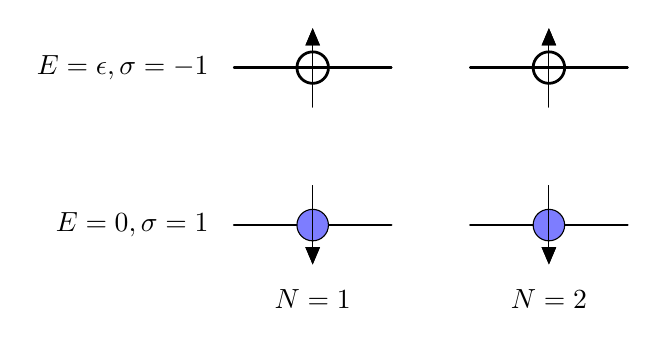
\begin{tikzpicture}[line cap=round,line join=round,>=triangle 45,x=1cm,y=1cm]
		 % Draw energy levels
	    \draw[thick] (0,0) -- (2,0);
	    \draw[thick] (3,0) -- (5,0);
	    \draw[thick] (0,2) -- (2,2);
	    \draw[thick] (3,2) -- (5,2);
	    
	    % Label energy levels
            \node[left] at (-0.2,0) {$E = 0, \sigma = 1$};
	    \node[left] at (-0.2,2) {$E = \epsilon, \sigma = -1$};

	    % Draw particles
	    \filldraw[fill=xdxdff] (1,0) circle (0.2);
	    \node[below] at (1,-0.7){$N = 1$};
	    \filldraw[fill=xdxdff] (4,0) circle (0.2);
	    \node[below] at (4, -0.7) {$N = 2$};

	    \draw[line width=1pt] (1,2) circle (0.2);
	    \draw[line width=1pt] (4,2) circle (0.2);

	    \draw[->] (1,0.5) -- (1,-0.5);
	    \draw[->] (4,0.5) -- (4,-0.5);
	    \draw[->] (1,0.5) -- (1,-0.5);
	    \draw[->] (4,0.5) -- (4,-0.5);
	
	    \draw[->] (1,1.5) -- (1,2.5);
	    \draw[->] (4,1.5) -- (4,2.5);
	    \draw[->] (1,1.5) -- (1,2.5);
	    \draw[->] (4,1.5) -- (4,2.5);
	\end{tikzpicture} 
	\caption{Illustration of the LMG model with $ 2 $ doubly degenerate single particle states and $ 2 $ particles.}
        \label{fig:lmg-illu}
\end{figure}


If $ \alpha_{p\sigma}^{\dagger} $ is the creation operator for a particle in the $ p $ state on the $ \sigma $ level, the Hamiltonian of the LMG model is given by
\begin{equation}
	\label{eq:lmg_hamiltonian}
	\begin{aligned}
		H_0 &= \varepsilon J_z, \\
		H_1 &= \frac{1}{2} V \sum_{p,p',\sigma} a_{p\sigma}^\dagger a_{p'\sigma}^\dagger a_{p'-\sigma} a_{p-\sigma}, \\
		H_{2} &= \frac{1}{2} W \sum_{p,p',\sigma}a_{p\sigma}^\dagger a_{p'-\sigma}^\dagger a_{p'\sigma}a_{p-\sigma},
	\end{aligned}
\end{equation}
where $ H_0 $ is a single particle term and $ H_1 $ and $ H_2 $ are the interaction terms. The total Hamiltonian is the sum of all three components,
\[ H = H_0+H_1+H_2. \] 

The Hamiltonian can be rewritten in terms of quasi-spin operators,

\begin{equation}
	\label{eq:Hqs}
	\begin{aligned}
		H_0 &= \varepsilon J_z,	\\
		H_1 &= \frac{1}{2} V \left( J_+^2 + J_-^2 \right),\\
		H_2 &= \frac{1}{2} W \left( -N + J_+ J_- + J_- J_+ \right),
	\end{aligned}
\end{equation} 

where the quasi-spin operators $ J_z, J_\pm $ are defined as 
\begin{equation}
	\begin{aligned}
		J_z &= \frac{1}{2} \sum_{p,\sigma} a_{p\sigma}^\dagger a_{p\sigma}, \\
		J_+ &= \sum_{p} a_{p\sigma}^\dagger a_{p-\sigma}, \\
		J_- &= \sum_{p} a_{p-\sigma}^\dagger a_{p\sigma}.
	\end{aligned}
\end{equation}

The quasi-spin operators satisfy the following relations
\begin{align}
	\label{eq:jrel}
		J_+ \vert J,J_z\rangle &= \sqrt{J(J+1) - J_z(J_z + 1)} \vert J,J_z + 1\rangle,\\
		J_- \vert J,J_z\rangle &= \sqrt{J(J+1) - J_z(J_z - 1)} \vert J,J_z - 1\rangle.
\end{align}
Instead of using the Jordan-Wigner transform to convert the second quantised Hamiltonian into a qubit Hamiltonian, these properties of the LMG model allow us to rewrite the Hamiltonian directly into Pauli matrices. We will discuss two cases for $ J=1 $ and $ J=2 $, then a discussion of the general case. 
\subsection{Case J=1}
\label{subsec:case_j1}
Acting with $ J_+ $ and $ J_- $ on all possible states to get the matrix elements:
\[ J_+ \ket{1,-1} = \sqrt{2}\ket{1,0}, \] 
\[ J_+ \ket{1,0} = \sqrt{2} \ket{1,1}, \] 
\[ J_+ \ket{1,1} = 0. \] 
We can obtain a set of similar relations for $ J_- $. Hence the matrix representation of the operators are
\begin{equation}
	J_z = 
	\begin{bmatrix}
		-1 & 0 & 0 \\
		0 & 0 & 0 \\
		0 & 0 & 1
	\end{bmatrix}, \quad
	J_+^2 = \begin{bmatrix}
		2 & 2 & 0 \\
		2 & 2 & 0 \\
		0 & 0 & 0
	\end{bmatrix}, \quad
	J_-^2  = \begin{bmatrix}
		0 & 0 & 0 \\
		0 & 2 & 2 \\
		0 & 2 & 2
	\end{bmatrix}.
\end{equation}
Substituting the matrix representations of the operators into Equation~\eqref{eq:Hqs}, we obtain
\begin{equation}
	\label{eq:j1mat}
	H_{J=1} = \begin{bmatrix}
		-\epsilon & 0 & v \\
		0 & W & 0 \\
		v & 0 & \epsilon
	\end{bmatrix}.
\end{equation}
We now want to rewrite the Hamiltonian in terms of Pauli matrices. We set $ W=0 $, then \[ H = H_0 + VH_1 \] 

\begin{equation}
	\label{eq:rewrite}
	\begin{aligned}
		J_z &= \sum_{n} j_z^{(n)} = \frac{1}{2} (Z_1+Z_2),\\
		\implies H_0 &= \epsilon J_z = \frac{\epsilon}{2} (Z_1+Z_2).
	\end{aligned}	
\end{equation}
\begin{equation}
	\label{eq:rewrite2}
	\begin{aligned}
		H_1 &= \frac{1}{2}V(J_+^2 + J_-^2), \\
		    &= \frac{1}{2}V \left[(\sum_n j_+^{(n)})^2 + (\sum_n j_-^{(n)})^2 \right] ,\\
		=& \frac{1}{2}V \left( \sum_{nm} \left( j_+^{(n)}j_+^{(m)} + j_-^{(n)}j_-^{(m)} \right)  \right), \\
		 &= \frac{1}{2}V \sum_{nm} \left( j_x + ij_y \right) ^{(n)}  \left( j_x + ij_y \right) ^{(m)} +  \left( j_x - ij_y \right) ^{(n)}  \left( j_x - ij_y \right) ^{(m)}, \\
		 &= \frac{1}{2} V \sum_{nm} (j_x^{(n)} j_x^{(m)} + ij_y^{(n)}j_x^{(m)} - j_y^{(n)} j_y^{(n)} + j_x^{(n)}j_x^{m} - ij_y^{n}j_x^{(m)} - j_y^{(n)}j_y^{(m)}),\\
	\end{aligned}	
\end{equation}
since 
\[j_x = \frac{X}{2}, j_y = \frac{Y}{2}, j_z = \frac{Z}{2}.\] 
Equation~\eqref{eq:rewrite} and ~\eqref{eq:rewrite2} becomes
\[ 
\begin{aligned}
	& v \sum_{nm} \left( j_x^{(n)}j_x^{(m)} - j_y^{(n)}j_y^{(m)} \right), \\
	&= 2v \sum_{n<m} \left( \frac{X_n}{2}\frac{X_m}{2} - \frac{Y_n}{2}\frac{Y_m}{2} \right).
\end{aligned}\] 
\begin{equation}
	\implies H_1 = \frac{1}{2} V (X_1 \otimes X_2  - Y_1 \otimes Y_2).
\end{equation}
Combining $ H_0 $ and $ H_1 $ 
\begin{equation}
	\label{eq:qubit-hamiltonian-j1-rewrite}
	H =  \frac{\epsilon}{2} (Z_1 + Z_2) + \frac{1}{2} V (X_1 \otimes X_2 - Y_1 \otimes Y_2).
\end{equation}



\subsection{Case J=2}
\label{subsec:case_j2}
Using again Equation~\eqref{eq:jrel}, we obtain the Hamiltonian matrix for $ J=2 $.
\begin{equation}
H_{J = 2} =
\begin{pmatrix}
-2\varepsilon & 0 & \sqrt{6}V & 0 & 0 \\
0 & -\varepsilon + 3W & 0 & 3V & 0 \\
\sqrt{6}V & 0 & 4W & 0 & \sqrt{6}V \\
0 & 3V & 0 & \varepsilon + 3W & 0 \\
0 & 0 & \sqrt{6}V & 0 & 2\varepsilon
\end{pmatrix}
\end{equation}
Since the Hamiltonian in terms of the quasi-spin operators is general regardless of the values of $ J $. We can rewrite the Hamiltonian in terms of the quasi-spin operators directly for the $ J=2 $ case.
Note that the $ H_0 $ is a one-body term, we take all linear combinations of the $ Z $ and $ I $, the identity operator with one $ Z $. The $ X $ and $ Y $ terms both act on two bodies, so we need to take all combinations of $ XX $ (or $ YY $ ) and $ II $. The tensor product $ \otimes $ sign is omitted for simplicity.
\begin{equation}
	\label{eq:qubit-hamiltonian-j2-rewrite}
	\begin{aligned}
		H &= \epsilon\left( ZIII + IZII + IIZI + IIIZ \right) \\
		  &+ \frac{V}{2} (XXII + XIXI + XIIX + IXXI + IXIX + IIXX) \\
		  &- \frac{V}{2} (YYII + YIYI + YIIY + IYYI + IYIY + IIYY)
	\end{aligned}
\end{equation}
Again, rewriting the Hamiltonian in terms of Pauli matrices allows us to perform quantum computations with them.

We could also rewrite $ H_2 $ in terms of the Pauli matrices. Then the second term can be rewritten in similar ways to $ H_1 $ 
\[ \implies H_2 = \frac{1}{2}W(XXII + \cdots IIXX + YYII \cdots IIYY). \]
Setting $ W=0 $, the Hamiltonian for the system is Equation~\eqref{eq:qubit-hamiltonian-j2-rewrite}.


\subsection{Level Mapping}
\label{subsec:level_mapping}
Level mapping uses the symmetry of the LMG Hamiltonian to reduce the dimension (number of qubits) required for the mapping. One way, perhaps the more natural way, to map the fermions is by using one qubit to represent a state $ (n,\sigma) $ where $ n $ is the particle slot and $ \sigma $ is the level (either spin up or down). This is the same idea as the Jordan-Wigner mapping, which is wasteful in this case due to the symmetry of the LMG model. In this mapping it requires $ 2N $ qubits to represent a system of $ N $ particles since there are 2 levels. \\
However, we know also that the LMG model does not permit the shift between particle slots, hence given an $ n $, both of the $ \sigma $'s can't be occupied at the same time. By taking advantage of this situation, we could consider the ``level mapping'', where we associate a qubit with a doublet, with 
\[ 
\begin{aligned}
\ket{0} &\longleftrightarrow \ket{n, -1} \\
\ket{1} &\longleftrightarrow \ket{n, +1}.
\end{aligned}\] 
This allows us to map two states to one qubit, requiring only $ N $ qubits for a system of $ N $ particles~\cite{Cervia21}. 

\subsection{Dimensionality Reduction for Pauli Decomposition}
\label{subsec:dim_reduction}
In the $ J=1 $ case, Equation~\eqref{eq:j1mat} has a redundant dimension in the $ W=0 $ case since the second row and column contain only $ 0 $ entries. This means we could effectively reduce the dimension of the matrix to $ 2 \times 2 $, as shown in Equation~\eqref{eq:reducej1} which means only one qubit is required to represent the system instead of two qubits. 

\begin{equation}
	\label{eq:reducej1}
	H_{J=1} = \begin{bmatrix}
		-\epsilon & v \\
		v & \epsilon
	\end{bmatrix}.
\end{equation}

For the $ J=2 $ case, whilst by setting $ W=0 $ we do not automatically reduce the dimension of the matrix, through exchanging rows and columns we could rewrite the matrix in a way that the
Hamiltonian is block diagonal, where the top left block of the Hamiltonian represents the cases where the values of $ J_z $ are even and the bottom right matrix represents the cases where the values of $ J_z $ are odd. This means that we could effectively write the Hamiltonian matrix as.
\begin{equation}
	\begin{pmatrix}	
	-2 \epsilon & \sqrt{6} V & 0 & 0 & 0 \\
	\sqrt{6} V & 4 W & \sqrt{6} V & 0 & 0 \\
	0 & \sqrt{6} V & 2 \epsilon & 0 & 0 \\
	0 & 0 & 0 & -\epsilon+3 W & 3 V \\
	0 & 0 & 0 & 3 V & \epsilon+3 W
	\end{pmatrix}.
\end{equation}
We will compare in Section~\ref{sec:LMG_result} the results of the LMG model using level mapping with Pauli Decomposition. 


\section{Pairing Model}
\label{sec:pairing_model}
The pairing model is a simple model of a system of fermions with pairing interaction, which consists of $ N $ doubly degenerate energy levels with equal spacing. It reduces the computation complexity while maintaining a grasp of the essential physics of the system. The theory of superconductivity in which electrons form cooper pairs is described by the pairing interaction known as the BCS model~\cite{Bardeen1957, Cooper1959}.

The pairing Hamiltonian is given by
\begin{align}
	\label{eq:pairing-hamiltonian}	
	\hat{H}_0&=\xi \sum_{p, \sigma}(p-1) \hat{a}_{p \sigma}^{\dagger} \hat{a}_{p \sigma}, \\
	\hat{V}&=-\frac{1}{2} g \sum_{p q} a_{p+}^{\dagger} a_{p-}^{\dagger} a_{q-} a_{q+}.
\end{align}
and the full Hamiltonian is \[ H = H_0 + V. \]
We will select a case of the pairing model with $ 4 $ single particle states and $ 4 $ particles. Without any constraint, the Hilbert space has size $\binom{8}{4} = 70 $. This would require at least $\lceil \log_2(70)\rceil = 7$ qubits to represent the system, which is too large to simulate locally. However, the pairing Hamiltonian allows us to reduce the dimension of the Hilbert space by restricting the system to have no broken pairs as in the middle figure of Figure~\ref{fig:pairing-model}. 


\begin{figure}[ht]
	\centering
	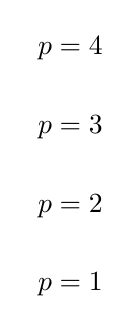
\begin{tikzpicture}
		\draw (0,-2) node[anchor=west] {$p=1$};
		\draw (0,-1) node[anchor=west] {$p=2$};
		\draw (0,0) node[anchor= west] {$p=3$};
		\draw (0,1) node[anchor= west] {$p=4$};
	\end{tikzpicture}
	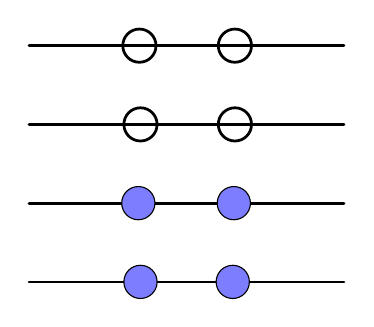
\begin{tikzpicture}[line cap=round,line join=round,>=triangle 45,x=1cm,y=1cm]
		%\clip(-3.4905745922175466,-9.485443631543706) rectangle (8.35815993106314,2.189471744302653);
		\draw [line width=1pt] (2,-2)-- (6,-2);
		\draw [line width=1pt] (2,-1)-- (6,-1);
		\draw [line width=1pt] (2,0)-- (6,0);
		\draw [line width=1pt] (2,1)-- (6,1);
		\draw [line width=1pt] (4.6143253381220655,0) circle (6pt);
		\draw [line width=1pt] (3.4151309606738582,0) circle (6pt);
		\draw [line width=1pt] (3.4013471172549132,1) circle (6pt);
		\draw [line width=1pt] (4.6143253381220655,1) circle (6pt);
		\begin{scriptsize}
		\draw [fill=xdxdff] (3.4151309606738582,-2) circle (6pt);
		\draw [fill=xdxdff] (4.5867576512841755,-2) circle (6pt);
		\draw [fill=xdxdff] (3.3875632738359682,-1) circle (6pt);
		\draw [fill=xdxdff] (4.600541494703121,-1) circle (6pt);
		\end{scriptsize}
	\end{tikzpicture} 
	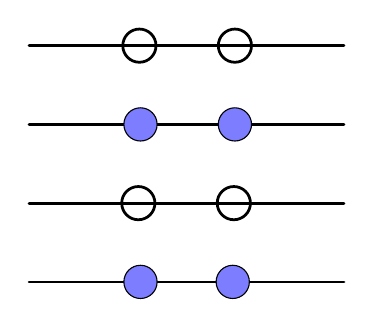
\begin{tikzpicture}[line cap=round,line join=round,>=triangle 45,x=1cm,y=1cm]
		%\clip(-3.4905745922175466,-9.485443631543706) rectangle (8.35815993106314,2.189471744302653);
		\draw [line width=1pt] (2,-2)-- (6,-2);
		\draw [line width=1pt] (2,-1)-- (6,-1);
		\draw [line width=1pt] (2,0)-- (6,0);
		\draw [line width=1pt] (2,1)-- (6,1);
		\draw [fill=xdxdff] (4.6143253381220655,0) circle (6pt);
		\draw [fill=xdxdff] (3.4151309606738582,0) circle (6pt);
		\draw [line width=1pt] (3.4013471172549132,1) circle (6pt);
		\draw [line width=1pt] (4.6143253381220655,1) circle (6pt);
		\begin{scriptsize}
		\draw [fill=xdxdff] (3.4151309606738582,-2) circle (6pt);
		\draw [fill=xdxdff] (4.5867576512841755,-2) circle (6pt);
		\draw [line width=1pt] (3.3875632738359682,-1) circle (6pt);
		\draw [line width=1pt] (4.600541494703121,-1) circle (6pt);
		\end{scriptsize}
	\end{tikzpicture} 
	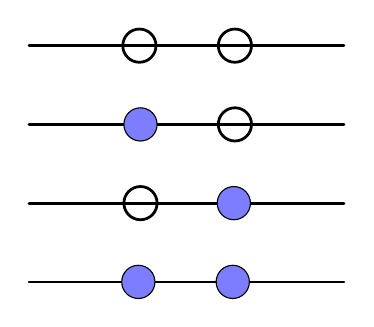
\begin{tikzpicture}[line cap=round,line join=round,>=triangle 45,x=1cm,y=1cm]
		%\clip(-3.4905745922175466,-9.485443631543706) rectangle (8.35815993106314,2.189471744302653);
		\draw [line width=1pt] (2,-2)-- (6,-2);
		\draw [line width=1pt] (2,-1)-- (6,-1);
		\draw [line width=1pt] (2,0)-- (6,0);
		\draw [line width=1pt] (2,1)-- (6,1);
		\draw [line width=1pt] (4.6143253381220655,0) circle (6pt);
		\draw [fill=xdxdff] (3.4151309606738582,0) circle (6pt);
		\draw [line width=1pt] (3.4013471172549132,1) circle (6pt);
		\draw [line width=1pt] (4.6143253381220655,1) circle (6pt);
		\begin{scriptsize}
		\draw [line width=1pt] (3.4151309606738582,-1) circle (6pt);
		\draw [fill=xdxdff] (4.5867576512841755,-2) circle (6pt);
		\draw [fill=xdxdff] (3.3875632738359682,-2) circle (6pt);
		\draw [fill=xdxdff] (4.600541494703121,-1) circle (6pt);
		\end{scriptsize}
	\end{tikzpicture} 
	\caption{Illustration of the pairing model with $ 4 $ doubly degenerate single particle states and $ 4 $ particles. The Left shows all the particles are in the lowest-lying states. The middle figure shows a doubly excited state where no pairs are broken. The right figure shows a state with a singly excited particle where a pair is broken.}
	\label{fig:pairing-model}
\end{figure}


Without loss of generality, we set $ \xi=1 $ and vary the value of $ g $, the pairing strength. 
Consider the spin project operator 
\begin{align}
	\label{eq:spin-proj}
	\hat{S}_z & =\frac{1}{2} \sum_{p, \sigma} \sigma \hat{a}_{p \sigma}^{\dagger} \hat{a}_{p \sigma}, \\ 
	\hat{S}^2 & =\hat{S}_z^2+\frac{1}{2}\left(\hat{S}_{+} \hat{S}_{-}+\hat{S}_{-} \hat{S}_{+}\right), \\ 
	\hat{S}_{\pm} & =\sum_p \hat{a}_{p \pm}^{\dagger} \hat{a}_{p \mp}.
\end{align}
The pair creation and annihilation operators are defined as 
\begin{equation}
	\label{eq:pairingCreAnn}
	\hat{P}_p^{+}=\hat{a}_{p+}^{\dagger} \hat{a}_{p-}^{\dagger}, \quad \hat{P}_p^{-}=\hat{a}_{p-} \hat{a}_{p+}.
\end{equation}
The pairing Hamiltonian can be rewritten as 

\begin{equation}
	\label{eq:pairing-inP}
	\hat{H}=\sum_{p \sigma}(p-1) a_{p \sigma}^{\dagger} a_{p \sigma}-\frac{1}{2} g \sum_{p q} \hat{P}_p^{+} \hat{P}_q^{-}.
\end{equation}
To set up the matrix Hamiltonian for where no pair is broken we need to set up the basis for the system. We include all possible combinations for the $ 4 $ particles to occupy the $ 4 $ doubly degenerate states without breaking any pairs as the basis. Such that
\begin{equation}
	\label{eq:pairing-basis}
	\begin{aligned}
		\ket{\phi_0} &= \ket{1_+,1_-,2_+,2_=} = \hat a_{2+}^{\dagger} \hat a_{2-}^{\dagger} \hat a_{1+}^{\dagger} \hat a_{1-}^{\dagger} = \hat P_{2}^{+} \hat P_{1}^{+} \ket{0}  \\
		\ket{\phi_1} &= \ket{1_+,1_-,3_+,3_-} = \hat P_{3}^{+} \hat P_{1}^{+} \ket{0} \\
		\ket{\phi_2} &= \ket{1_+,1_-,4_+,4_-} = \hat P_{4}^{+} \hat P_{1}^{+} \ket{0} \\
		\ket{\phi_3} &= \ket{2_+,2_-,3_+,3_-} = \hat P_{3}^{+} \hat P_{2}^{+} \ket{0} \\
		\ket{\phi_4} &= \ket{2_+,2_-,4_+,4_-}  = \hat P_{4}^{+} \hat P_{2}^{+} \ket{0} \\
		\ket{\phi_5} &= \ket{3_+,3_-,4_+,4_-} = \hat P_{4}^{+} \hat P_{3}^{+} \ket{0}.
	\end{aligned}
\end{equation}
Let 
\[ \left|\Phi_0\right\rangle=\left(\begin{array}{l}
1 \\
0 \\
0 \\
0 \\
0 \\
0
\end{array}\right), \quad\left|\Phi_1\right\rangle=\left(\begin{array}{l}
0 \\
1 \\
0 \\
0 \\
0 \\
0
\end{array}\right), \quad \cdots \quad\left|\Phi_5\right\rangle=\left(\begin{array}{l}
0 \\
0 \\
0 \\
0 \\
0 \\
1
\end{array}\right), \] 
be the basis for the system, and compute the matrix element $ \braket{\phi_i|\hat H|\phi_j} $ using Equation~\eqref{eq:pairingCreAnn}. We obtain that the matrix representation of the Hamiltonian
\begin{equation}
    \label{eq:pairing-mat}
	\hat{H}= \begin{pmatrix} 
	2-g & -g / 2 & -g / 2 & -g / 2 & -g / 2 & 0 \\
	-g / 2 & 4-g & -g / 2 & -g / 2 & 0 & -g / 2 \\
	-g / 2 & -g / 2 & 6-g & 0 & -g / 2 & -g / 2 \\
	-g / 2 & -g / 2 & 0 & 6-g & -g / 2 & -g / 2 \\
	-g / 2 & 0 & -g / 2 & -g / 2 & 8-g & -g / 2 \\
	0 & -g / 2 & -g / 2 & -g / 2 & -g / 2 & 10-g
	 \end{pmatrix}.
\end{equation}
We will encode this Hamiltonian using Pauli Decomposition into qubit Hamiltonian for the VQEs. The Hamiltonian has $ 18 $ terms.

The qubit Hamiltonian is given in Table~\ref{tab:pairing-qh}.

\begin{table}[ht]
    \centering
    \begin{tabular}{cc}
        \toprule
        \textbf{Pauli String} & \textbf{Coefficient} \\ 
        \midrule
        III & 28.5 \\ 
        IIX & -0.25 \\ 
        IIZ & -0.5 \\ 
        IXI & -0.25 \\ 
        IXX & -0.25 \\ 
        IZI & -23.5 \\ 
        IZX & -0.25 \\ 
        IZZ & -0.5 \\ 
        XII & -0.25 \\ 
        XXI & -0.25 \\ 
        XXX & -0.25 \\ 
        XZI & -0.25 \\ 
        YYI & -0.25 \\ 
        YYX & -0.25 \\ 
        ZII & -25 \\ 
        ZXI & -0.25 \\ 
        ZXX & -0.25 \\ 
        ZZI & 22 \\ 
        \bottomrule
    \end{tabular}
    \caption{Pauli strings and their coefficients.}
    \label{tab:pairing-qh}
\end{table}


\section{Deuteron Model}
\label{sec:deutron_model}

The deuteron model is a bound state of a proton and a neutron, which is surprisingly stable since neutrons are famously not~\cite{mit_deuteron}. We follow the derivation of the deuteron Hamiltonian as~\cite{Dumitrescu2018, Binder2016, Bansal2017} for our simulation, where a discrete variable representation in the harmonic oscillator basis is used. The Hamiltonian is given as
\begin{equation}
    \label{eq:deuteron-hamiltonian}
	H_N=\sum_{n, n^{\prime}=0}^{N-1}\left\langle n^{\prime}|(T+V)| n\right\rangle a_{n^{\prime}}^{\dagger} a_n.
\end{equation}
where $ n $ is the harmonic oscillator quantum number, $ a_n^\dagger, a_n $ are the creation and annihilation operators for the deuteron in the harmonic oscillator s-wave state $\ket{n} $, $ T $ is the kinetic energy operator and $ V $ is the potential energy operator. The kinetic energy operator $ T $ and potential energy operator $ V $ are given by 

\begin{equation}
	\begin{aligned}
	\left\langle n^{\prime}|T| n\right\rangle= & \frac{\hbar \omega}{2}\left[(2 n+3 / 2) \delta_n^{n^{\prime}}-\sqrt{n(n+1 / 2)} \delta_n^{n^{\prime}+1}\right. \left.-\sqrt{(n+1)(n+3 / 2)} \delta_n^{n^{\prime}-1}\right], \\
	\left\langle n^{\prime}|V| n\right\rangle= & V_0 \delta_n^0 \delta_n^{n^{\prime}},
	\end{aligned}
\end{equation}
where $V_0 = -5.68658111 $ MeV and $ \hbar \omega = 7 $ MeV.

The Jordan-Wigner transform was used in \cite{Dumitrescu2018} to map the Deuteron Hamiltonian to qubit Hamiltonian. Glancing through Equation~\eqref{eq:deuteron-hamiltonian} yields that it does not have any two-body term, which means transforming it with Jordan-Wigner transformation is wasteful. However, rewriting it into a Hamiltonian matrix and then using the Pauli decomposition saves the number of qubits required to represent the system. This is a huge advantage for any algorithm running on NISQ devices, especially since the basis dimension $ N $ can increase indefinitely. Since we are able to save on the number of qubits we will push the basis dimension $ N $ to higher values than the $ N=3 $ in the original paper.


\part{Results and Discussion}
\chapter{Results}
\label{chap:results}
In this chapter, we present results from both exact energy simulations (with no shot noise) and ideal simulations (with shot noise) for the Hydrogen molecule, LMG model, Pairing model and the Deuteron model discussed in the previous chapter. The results are grouped based on the models they belong to and the analysis of properties for the qubit-ADAPT-VQE and the fixed-form ansatz are distributed into different sections. 
When a result is produced ``without shot noise'', the analytical expression for the energy is calculated. This is equivalent to taking \texttt{n\_shots} $ \to \infty $. The optimisers are methods from \texttt{scipy.optimize.minimize}. If the exponential decomposition method is not mentioned explicitly, the inverted staircase algorithm described in Subsection~\ref{sub:invertedstaircase} is used. If the initialisation of a state is not mentioned explicitly, it is initialised in the maximally superposed state.

\section{Expected Error}
\label{sec:exp_error}
Even with our simulations being ideal, the energy estimations are not exact. Therefore, the best result one aims to achieve is the one whose energy error is at its theoretical minimum, i.e. only comes from shot noise. As described in Section~\ref{sub:shot_noise}, the error obtained from one measurement is given by 
\begin{equation}
	\label{eq:shot_noise}
	\epsilon \propto \sqrt{\frac{1}{N}},
\end{equation}
where $ N $ is the number of shots. 

For a qubit Hamiltonian with $ t $ terms, we define the expected error $ E_\epsilon $ error as
\[ E_{\epsilon}= \sqrt{t} \epsilon. \]


The maximum number of terms of Pauli strings a qubit Hamiltonian contains for an $n $ qubit system, is $ 4^n $. For example, the maximum number of terms for a $3$-qubit system is $64$. In most simulations, we have used $10^5$ shots. With $64$ Pauli strings of a three-qubit system, the shot noise then becomes
\[  \epsilon \propto \sqrt{\frac{64}{10^5}} \approx 0.025 \sim \mathcal{O}(10^{-2}).\]
Although the system usually does not contain all possible terms, this assessment will be done for every system separately as a reference point for the results.

\section{Run Time}
\label{sec:runtime}
The time taken to run each simulation is highly related to the number of shots, the size of the Hamiltonian and the number of objective function calls during the classical optimisation process. The time taken for the measurement scales linearly with the number of shots, as can be seen in Figure~\ref{fig:timed_shots}.
\begin{figure}[ht]
	\centering
	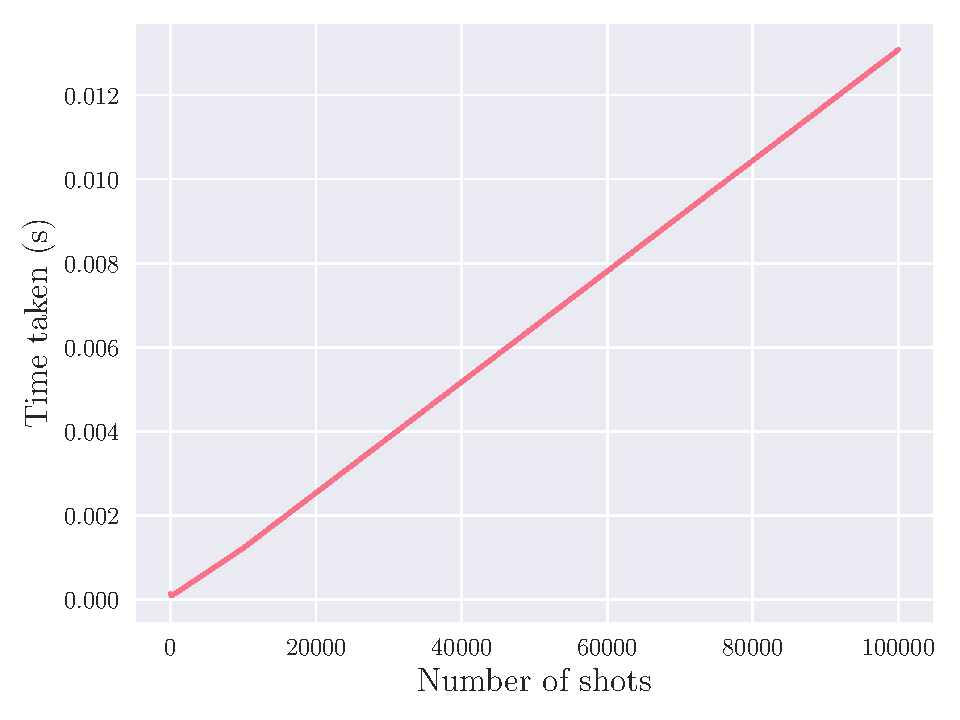
\includegraphics[width=0.7\linewidth]{image/time_vs_shots.pdf}
	\caption{Time taken in seconds for the measurement process as a function of the number of shots.}
	\label{fig:timed_shots}
\end{figure}

The time taken for every measurement with $ 10^5 $ shot is around $ 0.008374 s$. The total time taken for every calculation should also depend on the number of function calls and the length of the qubit Hamiltonian. 



\section{State Initialisation for ADAPT-VQE}
\label{sec:initstate}
According to~\cite{tang2021}, the operator pools $V$ and $G$ should be complete, i.e. any real state $ \ket{\psi} $ can be rotated to another state $ \ket{ \phi} $ with
\begin{equation}
	\ket{\phi} = \prod_{k} e^{\theta V_k} \ket{\psi}.
\end{equation}
However, the ADAPT-VQE stops when the gradient is $ 0 $ or below a certain threshold. Even after removing the even Pauli strings, i.e. Pauli string with an even number of $ Y $ operators, the operator gradient can still vanish for some states $ \ket{\psi}  $. Most noticeably, the $ \ket{0 \ldots 0} $ state. We will provide an example of where all the gradients of the operators vanish, and the ADAPT process stops after one iteration without converging to the correct state. 

For the case of three qubits, the complete $ V $ pool is $ \{ V \} = \{iYZZ, iIYZ, iIIY, iIYI\}$. The term $iYZZ$ can be written in matrix notation as Equation~\eqref{eq:matrixiYZZ}.
\begin{equation}
	\label{eq:matrixiYZZ}
	iYZZ = \begin{pmatrix}
	0 & 0 & 0 & 0 & 1 & 0 & 0 & 0 & \\ 
	0 & 0 & 0 & 0 & 0 & -1 & 0 & 0 & \\ 
	0 & 0 & 0 & 0 & 0 & 0 & -1 & 0 & \\ 
	0 & 0 & 0 & 0 & 0 & 0 & 0 & 1 & \\ 
	-1 & 0 & 0 & 0 & 0 & 0 & 0 & 0 & \\ 
	0 & 1 & 0 & 0 & 0 & 0 & 0 & 0 & \\ 
	0 & 0 & 1 & 0 & 0 & 0 & 0 & 0 & \\ 
	0 & 0 & 0 & -1 & 0 & 0 & 0 & 0 & \\ 
	\end{pmatrix}.
\end{equation}


Initialising the state $\ket{\psi}$
\[ \ket{\psi} = \ket{000}, \] 
for the operator selection process, we then calculate the gradient of each operator in the pool for an arbitrary Hamiltonian with real coefficients, which is true when time-reversal symmetry is preserved. The Hamiltonian of choice is
\begin{equation}
	\label{eq:0gradHamiltonian}
	H = 2IIZ - 0.5IXX + 0.5IYY + 2 ZZI
\end{equation}
in matrix notation that is
\begin{equation}
	\label{eq:0gradHmat}
\begin{pmatrix}
4 & 0 & 0 & -1 & 0 & 0 & 0 & 0  \\
0 & 0 & 0 & 0 & 0 & 0 & 0 & 0  \\
0 & 0 & 0 & 0 & 0 & 0 & 0 & 0  \\
-1 & 0 & 0 & -4 & 0 & 0 & 0 & 0  \\
0 & 0 & 0 & 0 & 0 & 0 & 0 & -1  \\
0 & 0 & 0 & 0 & 0 & -4 & 0 & 0  \\
0 & 0 & 0 & 0 & 0 & 0 & 4 & 0  \\
0 & 0 & 0 & 0 & -1 & 0 & 0 & 0  \\
\end{pmatrix}	
\end{equation}
The gradient is calculated using Equation~\eqref{eq:selection-criteria}. The commutator $ [H,A] $ with $ A=iYZZ $ is then

\begin{align*}
	[H,A] = HA-AH &=
	\begin{pmatrix}
4 & 0 & 0 & -1 & 0 & 0 & 0 & 0  \\
0 & 0 & 0 & 0 & 0 & 0 & 0 & 0  \\
0 & 0 & 0 & 0 & 0 & 0 & 0 & 0  \\
-1 & 0 & 0 & -4 & 0 & 0 & 0 & 0  \\
0 & 0 & 0 & 0 & 0 & 0 & 0 & -1  \\
0 & 0 & 0 & 0 & 0 & -4 & 0 & 0  \\
0 & 0 & 0 & 0 & 0 & 0 & 4 & 0  \\
0 & 0 & 0 & 0 & -1 & 0 & 0 & 0  \\
\end{pmatrix}
\begin{pmatrix}
0 & 0 & 0 & 0 & 1 & 0 & 0 & 0  \\
0 & 0 & 0 & 0 & 0 & -1 & 0 & 0  \\
0 & 0 & 0 & 0 & 0 & 0 & -1 & 0  \\
0 & 0 & 0 & 0 & 0 & 0 & 0 & 1  \\
-1 & 0 & 0 & 0 & 0 & 0 & 0 & 0  \\
0 & 1 & 0 & 0 & 0 & 0 & 0 & 0  \\
0 & 0 & 1 & 0 & 0 & 0 & 0 & 0  \\
0 & 0 & 0 & -1 & 0 & 0 & 0 & 0  \\
\end{pmatrix} \\ 
		      &- \begin{pmatrix}
0 & 0 & 0 & 0 & 1 & 0 & 0 & 0  \\
0 & 0 & 0 & 0 & 0 & -1 & 0 & 0  \\
0 & 0 & 0 & 0 & 0 & 0 & -1 & 0  \\
0 & 0 & 0 & 0 & 0 & 0 & 0 & 1  \\
-1 & 0 & 0 & 0 & 0 & 0 & 0 & 0  \\
0 & 1 & 0 & 0 & 0 & 0 & 0 & 0  \\
0 & 0 & 1 & 0 & 0 & 0 & 0 & 0  \\
0 & 0 & 0 & -1 & 0 & 0 & 0 & 0  \\
\end{pmatrix}
\begin{pmatrix}
4 & 0 & 0 & -1 & 0 & 0 & 0 & 0  \\
0 & 0 & 0 & 0 & 0 & 0 & 0 & 0  \\
0 & 0 & 0 & 0 & 0 & 0 & 0 & 0  \\
-1 & 0 & 0 & -4 & 0 & 0 & 0 & 0  \\
0 & 0 & 0 & 0 & 0 & 0 & 0 & -1  \\
0 & 0 & 0 & 0 & 0 & -4 & 0 & 0  \\
0 & 0 & 0 & 0 & 0 & 0 & 4 & 0  \\
0 & 0 & 0 & 0 & -1 & 0 & 0 & 0  \\
\end{pmatrix} \\
	&= \begin{pmatrix} 
	0 & 0 & 0 & 0 & 4 & 0 & 0 & 0  \\
	0 & 0 & 0 & 0 & 0 & -4 & 0 & 0  \\
	0 & 0 & 0 & 0 & 0 & 0 & 4 & 0  \\
	0 & 0 & 0 & 0 & 0 & 0 & 0 & -4  \\
	4 & 0 & 0 & 0 & 0 & 0 & 0 & 0  \\
	0 & -4 & 0 & 0 & 0 & 0 & 0 & 0  \\
	0 & 0 & 4 & 0 & 0 & 0 & 0 & 0  \\
	0 & 0 & 0 & -4 & 0 & 0 & 0 & 0 
	\end{pmatrix}.
\end{align*}
and 
\begin{align}
	\label{eq:zerograd}
	\braket{\psi|[H,A]|\psi} &= 
	\begin{pmatrix} 1 & 0 & 0 & 0 & 0 & 0 & 0 & 0  \end{pmatrix} 
	\begin{pmatrix} 
	0 & 0 & 0 & 0 & 4 & 0 & 0 & 0  \\
	0 & 0 & 0 & 0 & 0 & -4 & 0 & 0  \\
	0 & 0 & 0 & 0 & 0 & 0 & 4 & 0  \\
	0 & 0 & 0 & 0 & 0 & 0 & 0 & -4  \\
	4 & 0 & 0 & 0 & 0 & 0 & 0 & 0  \\
	0 & -4 & 0 & 0 & 0 & 0 & 0 & 0  \\
	0 & 0 & 4 & 0 & 0 & 0 & 0 & 0  \\
	0 & 0 & 0 & -4 & 0 & 0 & 0 & 0 
	\end{pmatrix}
	\begin{pmatrix} 1 \\ 0 \\ 0 \\ 0 \\ 0 \\ 0 \\ 0 \\ 0 \end{pmatrix}, \\
	&= \begin{pmatrix} 1 & 0 & 0 & 0 & 0 & 0 & 0 & 0 \end{pmatrix} 
	\begin{pmatrix} 0 \\ 0 \\ 0 \\ -1 \\ 4 \\ 0 \\ 0 \\ 0 \end{pmatrix}, \\
		&= 0.
\end{align}

In Appendix~\ref{app:zerograd} we will show that this is true for all the rest of the operators in the pool when the state $ \ket{000}$ is not the ground state for the system given by Equation~\eqref{eq:0gradHamiltonian}. The initialisation of the state is therefore crucial. We found that by starting in the maximally superposed state, $\ket{+}^{\otimes n}$, the gradients of the operators are non-zero, and the system does converge to the ground state eventually. This will therefore be the choice of initial state for the ADAPT-VQE from now on.

\section{Hydrogen Molecule}
\label{sec:hydrogen_result}

While producing results for the hydrogen molecule, we found that initialising the state in the Hartree-Fock state ($ \ket{1100} $in this case) results in the $ 0 $ gradient problem as described in Section~\ref{sec:initstate} and Appendix~\ref{app:zerograd}. Indeed, all terms of the qubit Hamiltonian shown in Table~\ref{tab:qubit-hamiltonian-h2} do not contribute to the gradient when the state is in the $ \ket{1100} $ or the $ \ket{0000} $ state. 

The qubit Hamiltonian contains $ 15 $ terms. The expected error for $ 10^5 $ shots is $ 0.00316 $. The expected error for the hydrogen molecule is therefore $ 0.012 $. 


\subsection{Exact Energy Simulation}
\begin{figure}[ht]
    \centering
    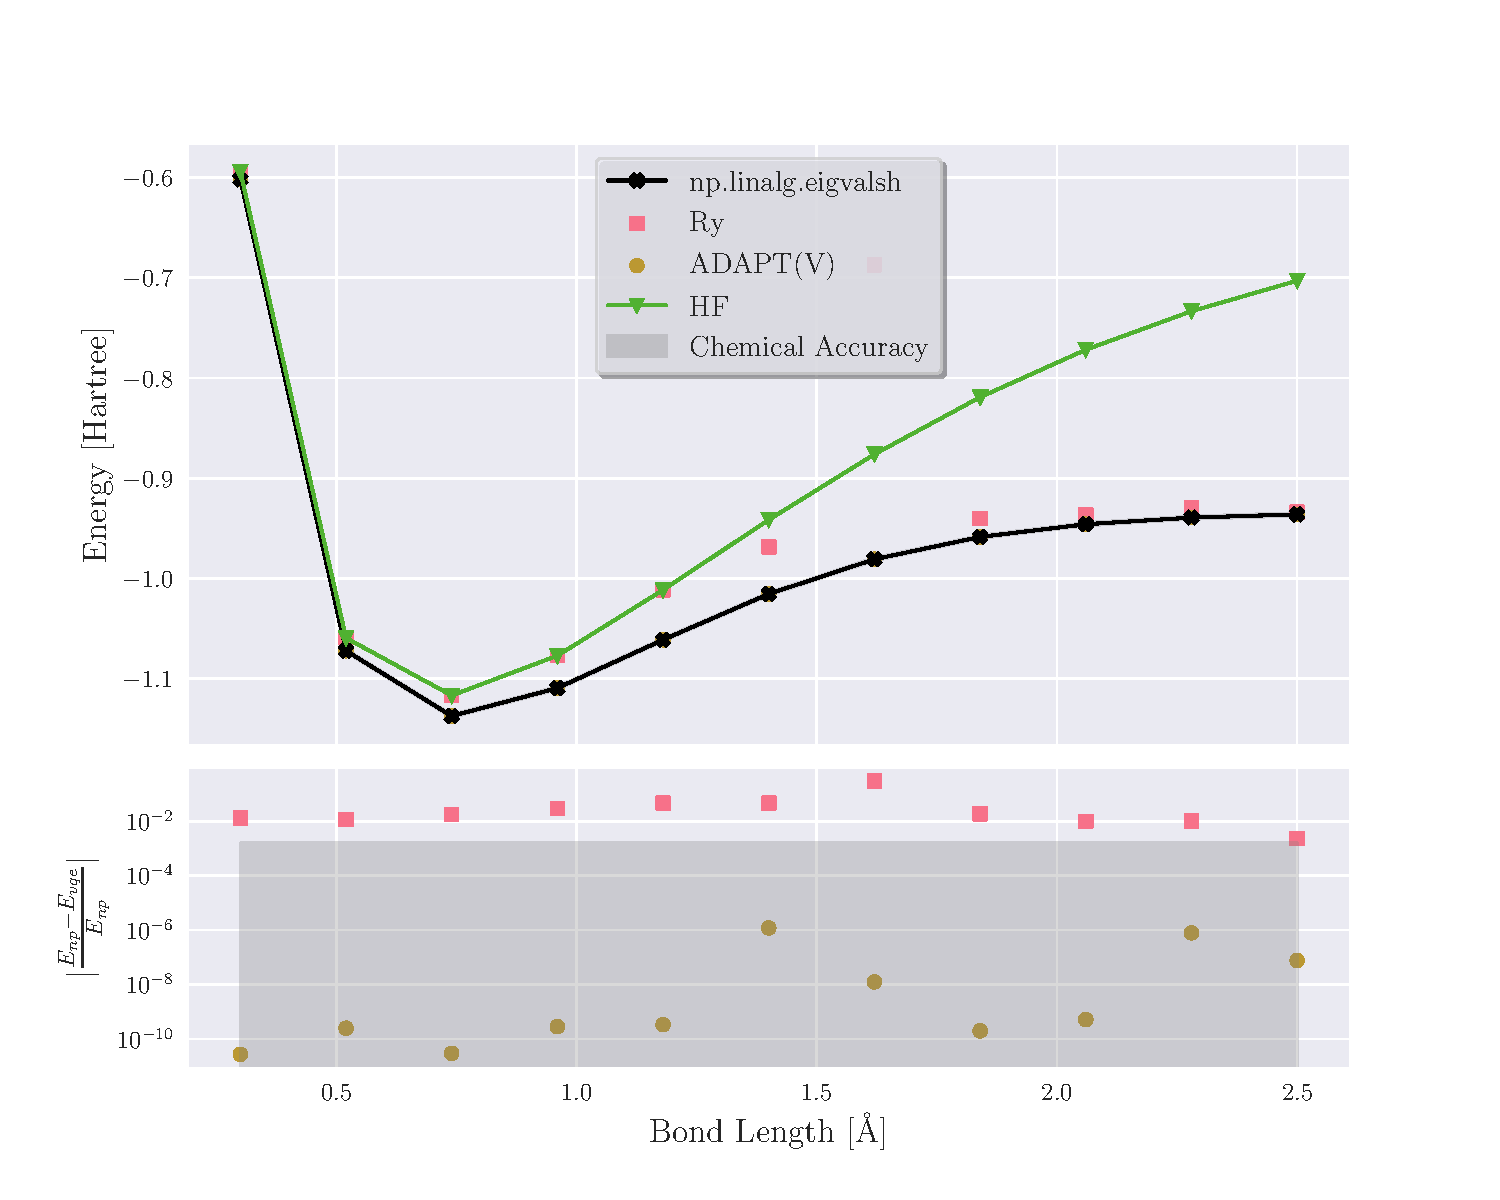
\includegraphics[width=\linewidth]{image/h2_result/nsn/best-nsn.pdf}
    \caption{The Hydrogen molecule with \textbf{exact energy simulation}, showing the comparison between VQE with $ 3 $ repetition and ADAPT-VQE with the $ V $ pool and maximum $ 30 $ ADAPT iterations. Both are minimised using the \texttt{BFGS} method. The VQE was initialised in the HF state and the ADAPT-VQE was initialised in a random real state. The yellow markers are hard to see on the upper plot as they are almost perfectly aligned with the numerical diagonalisation.}
    \label{fig:h2main-nsn}
\end{figure}

We see for the exact energy simulation that the ADAPT-VQE outperforms the VQE and Hartree-Fock by a large margin, and was able to converge to the exact diagonalisation result with an error within orders of $ 10^{-6} $ for both small and large bond length, also achieving chemical accuracy. The Ry ansatz was not able to converge to the true ground state for a small bond length, rather it converges to the HF state. This might be related to the Hartree-Fock initialisation. For large bond lengths where the Hartree-Fock energy is a poor estimation of the ground state, both VQEs exhibit better results than the Hartree-Fock energy. We also note that the performance of the ADAPT-VQE is not affected by the bond length as the error stays the same, suggesting that the qubit-ADAPT ansatz is exact and can represent the ground state with different interactions.


\subsection{Ideal Simulation}
\begin{figure}[ht]
    \centering
    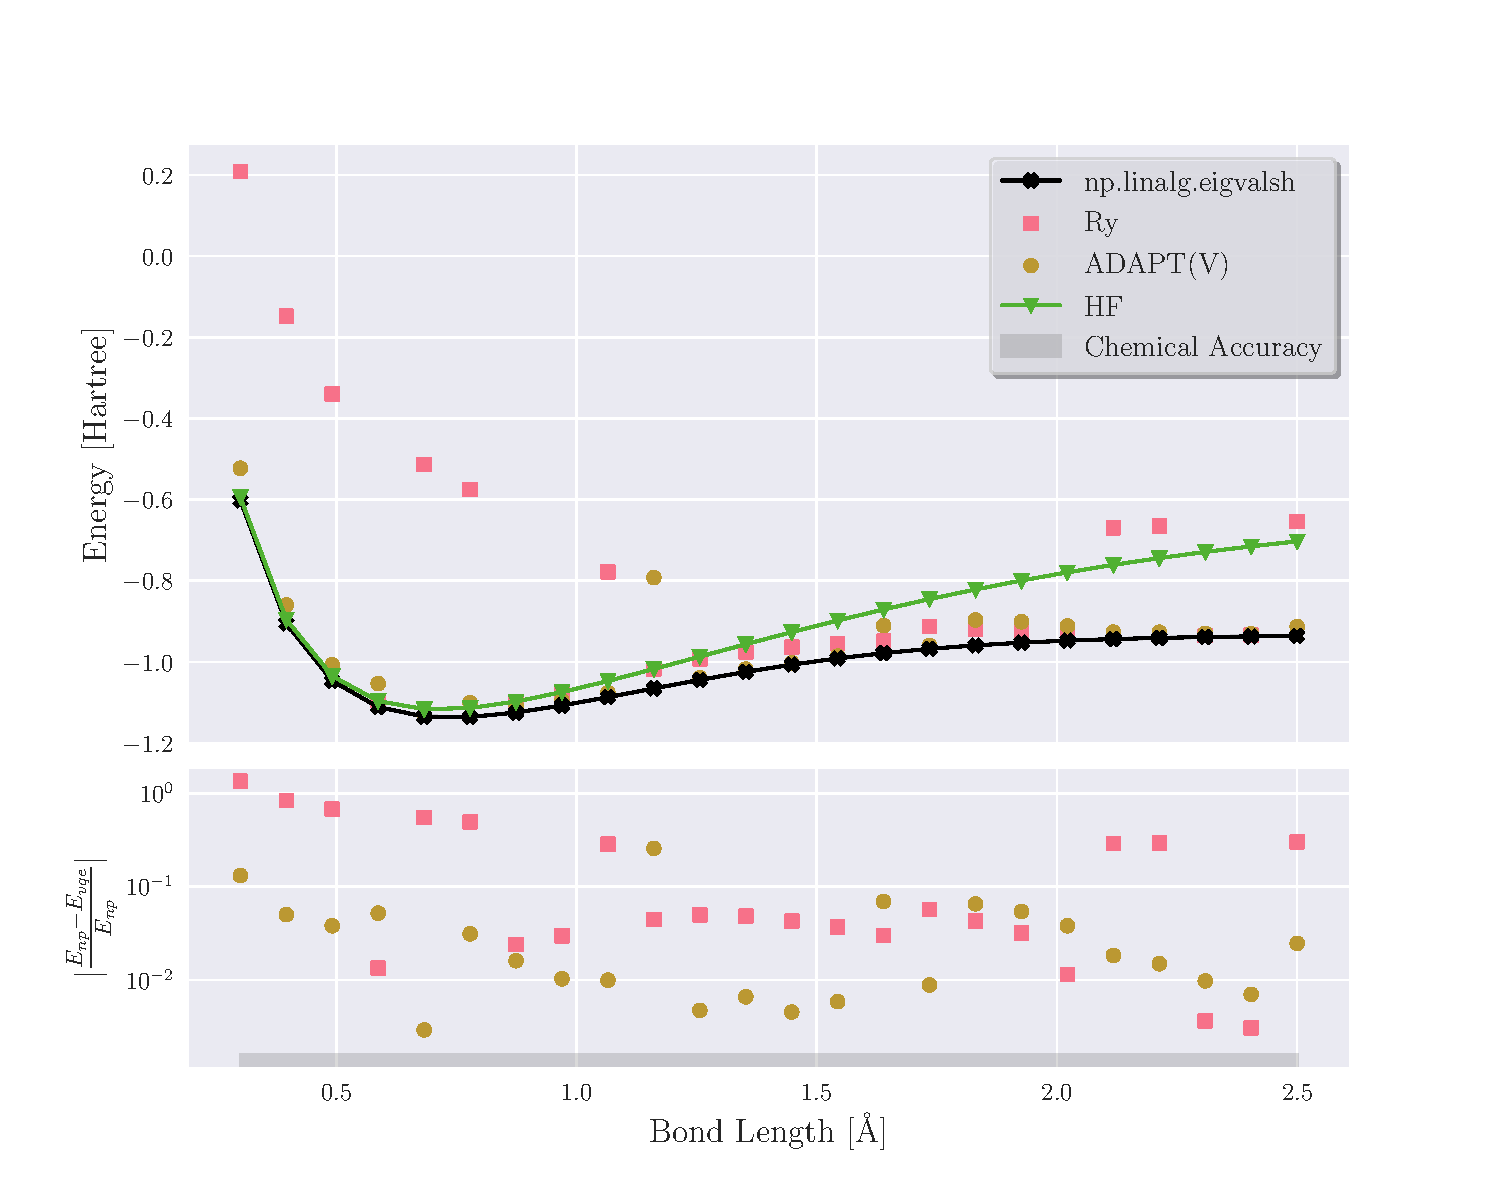
\includegraphics[width=\linewidth]{image/h2_result/simulation/best_sim.pdf}
    \caption{The hydrogen molecule with \textbf{ideal simulation} with $ 100000 $ shots for a maximum of $ 30 $ ADAPT iterations. The ADAPT-VQEs were optimised with the \texttt{COBYLA} method and the VQE with the \texttt{Powell} method. The exponential was decomposed using the \textbf{inverted Staircase} algorithm.}
    \label{fig:h2main-noisy}
\end{figure}

Figure~\ref{fig:h2main-noisy} shows the results for an ideal simulation. Again, ADAPT outperformed the VQE but the results for both were underwhelming and were not chemically accurate. It is still obvious that the ADAPT-VQE is more consistent in terms of performance when it comes to bond length, and the normal VQE with Ry ansatz performs poorly for both low and high bond lengths. Compared with the expected error with this shot noise $ 0.012 $, only a few points between $ 1 - 1.5 \text{Å} $ with the use of the ADAPT-VQE were able to obtain errors of the same magnitude.
The simple shot noise affects the convergence of the ADAPT-VQE greatly. Even with the ADAPT gradient being calculated analytically, the impact of the shot noise is still significant. We hypothesise that the optimisation for the VQE subroutine at every ADAPT iteration might not always converge, causing the state to be in a different state than the state with the optimal parameters for the current iteration. One suggestion to improve the result is to group commuting operators to be measured together to reduce the number of state preparations required.

To test our hypothesis, we ran the system with the same parameters except increasing the maximum iteration to $ 60 $. The result for this is shown in Figure~\ref{fig:60iterh2}. While this did not improve our results it helps us understand the problem better. For all the values, the energy was decreasing with every iteration initially but stopped after $ 10 $ iterations. For the case of $ 0.3 \text{Å} $, the error is below the expected error for the number of shots we use, as we can see from the fluctuation of the error after the convergence. For other bond lengths, however, the results were not able to reach the exact ground state as while more operators were being appended, the error was not decreasing to below the expected error. Meanwhile, the gradient is not small enough for the ADAPT-VQE to stop, which may suggest that with shot noise, the operator gradient might have trouble selecting the operator which changes the state the most. This also tells us that using the expected error is a good metric to evaluate the performance of an ideal simulation. This, incidentally, also results in a large increase of function calls, approximately $ 15000 $, where $ \sim 1000 $ function calls were made for the $ 15 $ iteration case and $ \sim 5000 $ for the $ 30 $ iteration case. This is a sign that the optimisers struggle as the number of parameters increases, which is unsurprising. 

\section{Lipkin-Meshkov-Glick Model}
\label{sec:LMG_result}
Here we showcase results obtained from both exact energy and ideal simulation for the LMG model, for both the $ J=1 $ and $ J=2 $ cases. We will assume $ W=0 $ throughout this section. 

The rewritten and Pauli decomposed Hamiltonian for $ J=1 $ has four terms, and $ J=2 $ has $ 16 $ terms. The expected error for these cases with $ 10^5 $ shots are $ 0.006 $ and $ 0.013 $ respectively. 


\subsection{Exact Energy Simulation}
Figure~\ref{fig:j1main-nsn} and Figure~\ref{fig:j2main-nsn} show the comparison between VQE and ADAPT-VQE for the LMG model with $ J=1 $ and $ J=2 $ for the \textbf{exact energy simulation}, respectively. We found that with $ repetition=1 $, the VQE algorithm was able to converge, but an attempt to improve the result further by adding another layer of gates caused the algorithm to fail to converge completely for the case of rewritten Hamiltonian as shown in Figure~\ref{fig:2repnotok}. For $ J=1 $, apart from a few points where one method did not converge, the convergence was decent for all the methods, with errors in orders of $ 10^{-8} $.  For the $ J=2 $ case the ADAPT with Pauli decomposed energy produced the best results with errors orders of $ 10^{-8} $ while other methods had errors between $ 10^{-2} $ and $ 10^{-1} $. In both cases, the ADAPT performed better than the VQE respectively by being more stable for all interaction strength and lower error. 

\begin{figure}[ht]
	\centering
	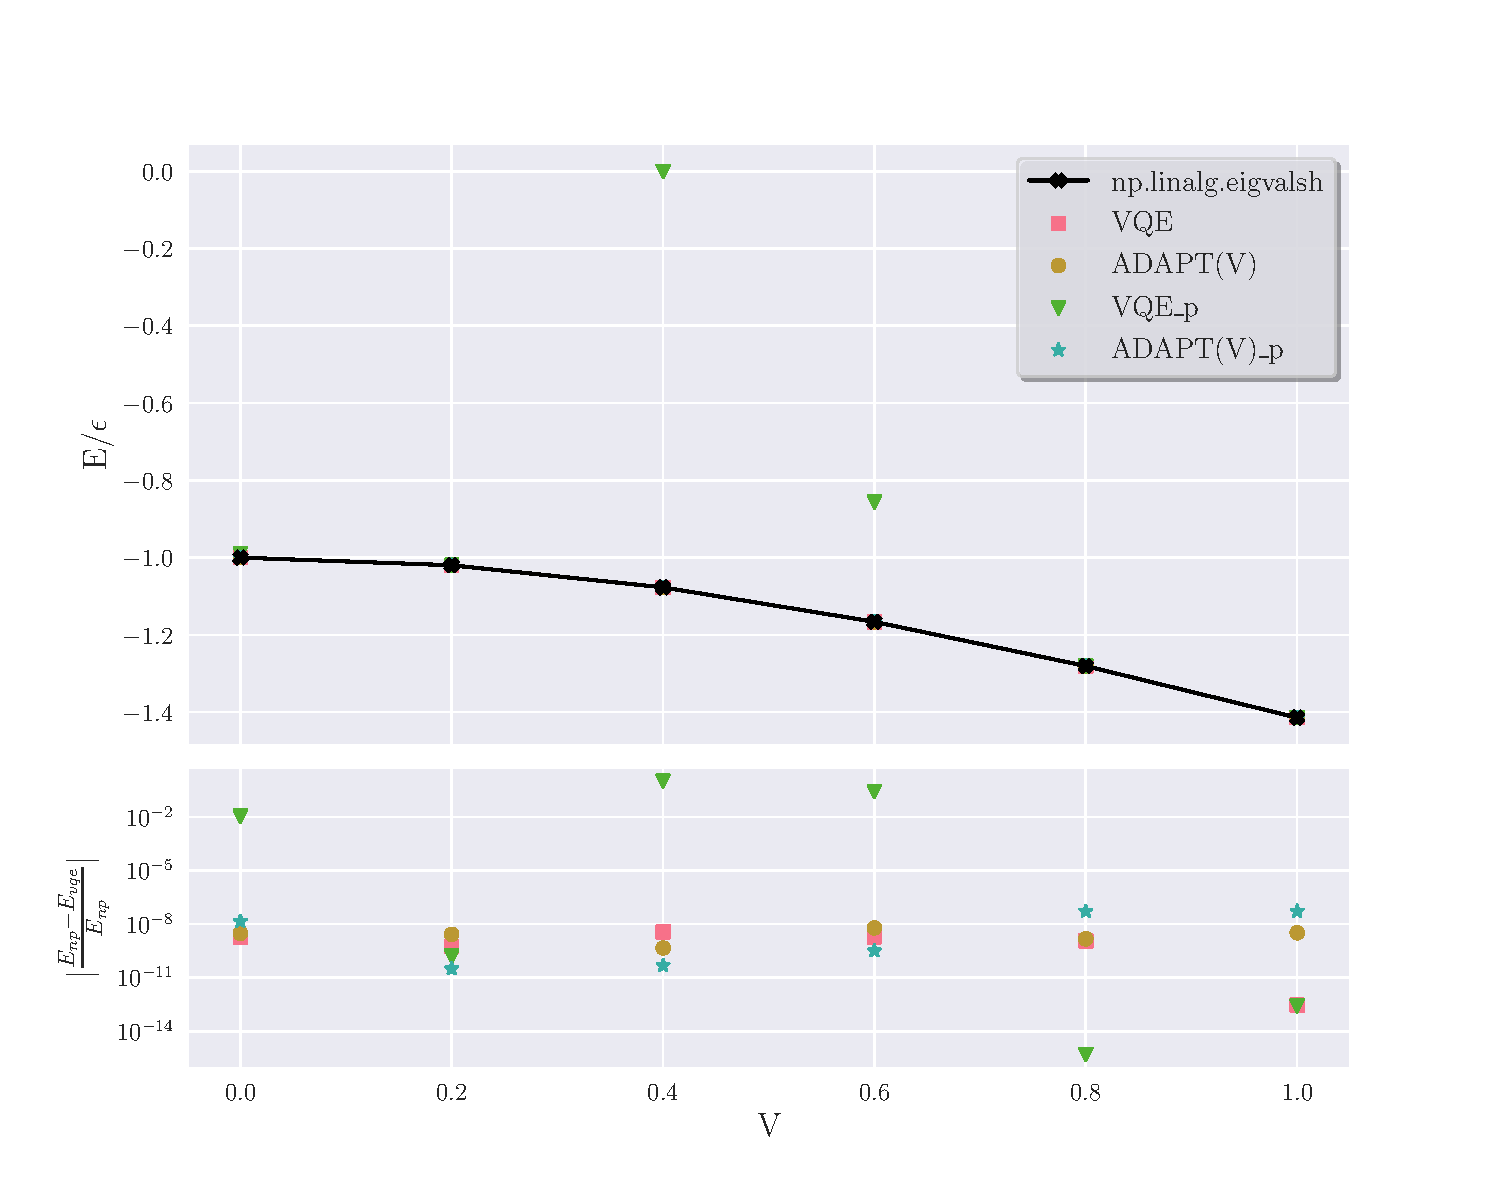
\includegraphics[width=\linewidth]{image/lipkin_result/j1main_False.pdf}
	\caption{The LMG model with $ J=1 $ with \textbf{exact energy simulation}, showing the comparison between VQE with $ 1 $ repetition and ADAPT-VQE with the $ V $  pool and maximum $ 12 $ ADAPT iterations. The label with \textit{\_p} means that the Hamiltonian was mapped using Pauli decomposition, otherwise, Equation~\eqref{eq:rewrite} was used. Both were optimised with \texttt{BFGS} method.}
	\label{fig:j1main-nsn}
\end{figure}

\begin{figure}[ht]
	\centering
	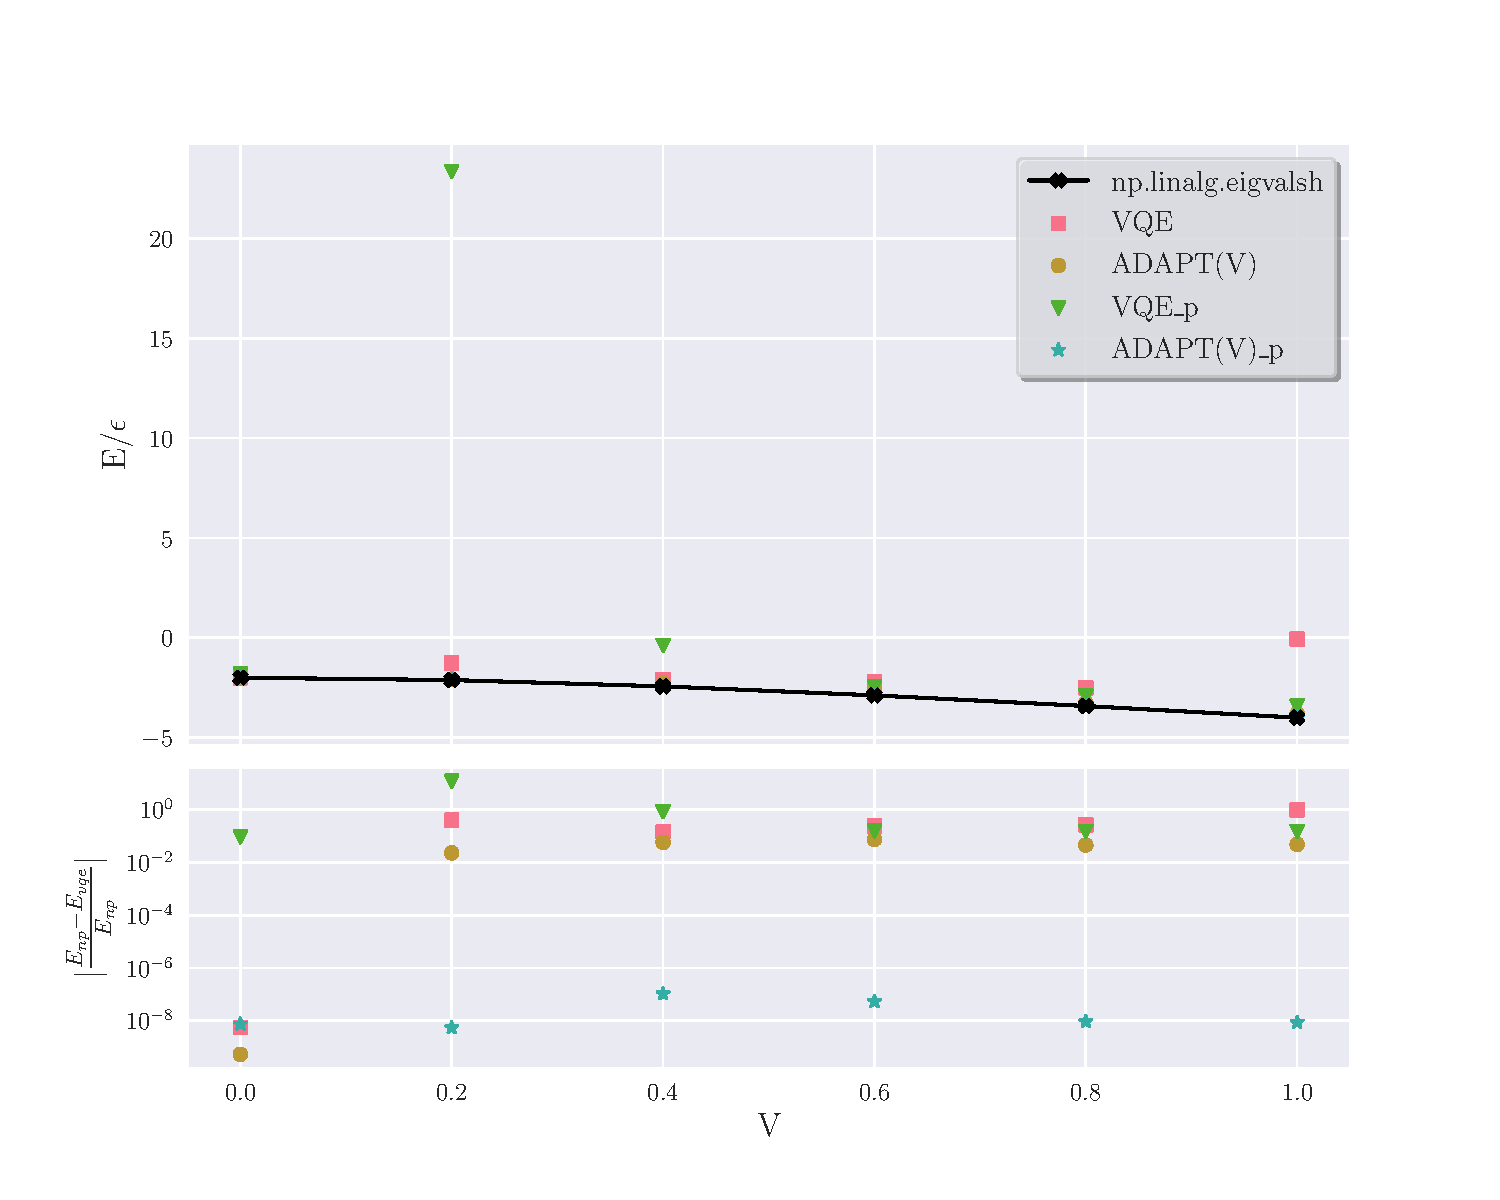
\includegraphics[width=\linewidth]{image/j2main_False.pdf}
	\caption{The LMG model with $ J=2 $ with \textbf{exact energy simulation}, showing the comparison between VQE with $ 1 $ repetition and ADAPT-VQE with the $ V $  pool and maximum $ 12 $ ADAPT iterations. Both were optimised with \texttt{BFGS} method. The label with \textit{\_p} means that the Hamiltonian was mapped using Pauli decomposition, otherwise, Equation~\eqref{eq:rewrite} was used.}
	\label{fig:j2main-nsn}
\end{figure}


\subsection{Ideal Simulation}
Figures~\ref{fig:j1main-noisy} and~\ref{fig:j2main-noisy} show the results for ideal simulations again for both $ J=1,2 $ as well as both mapping.
\begin{figure}[ht]
    \centering
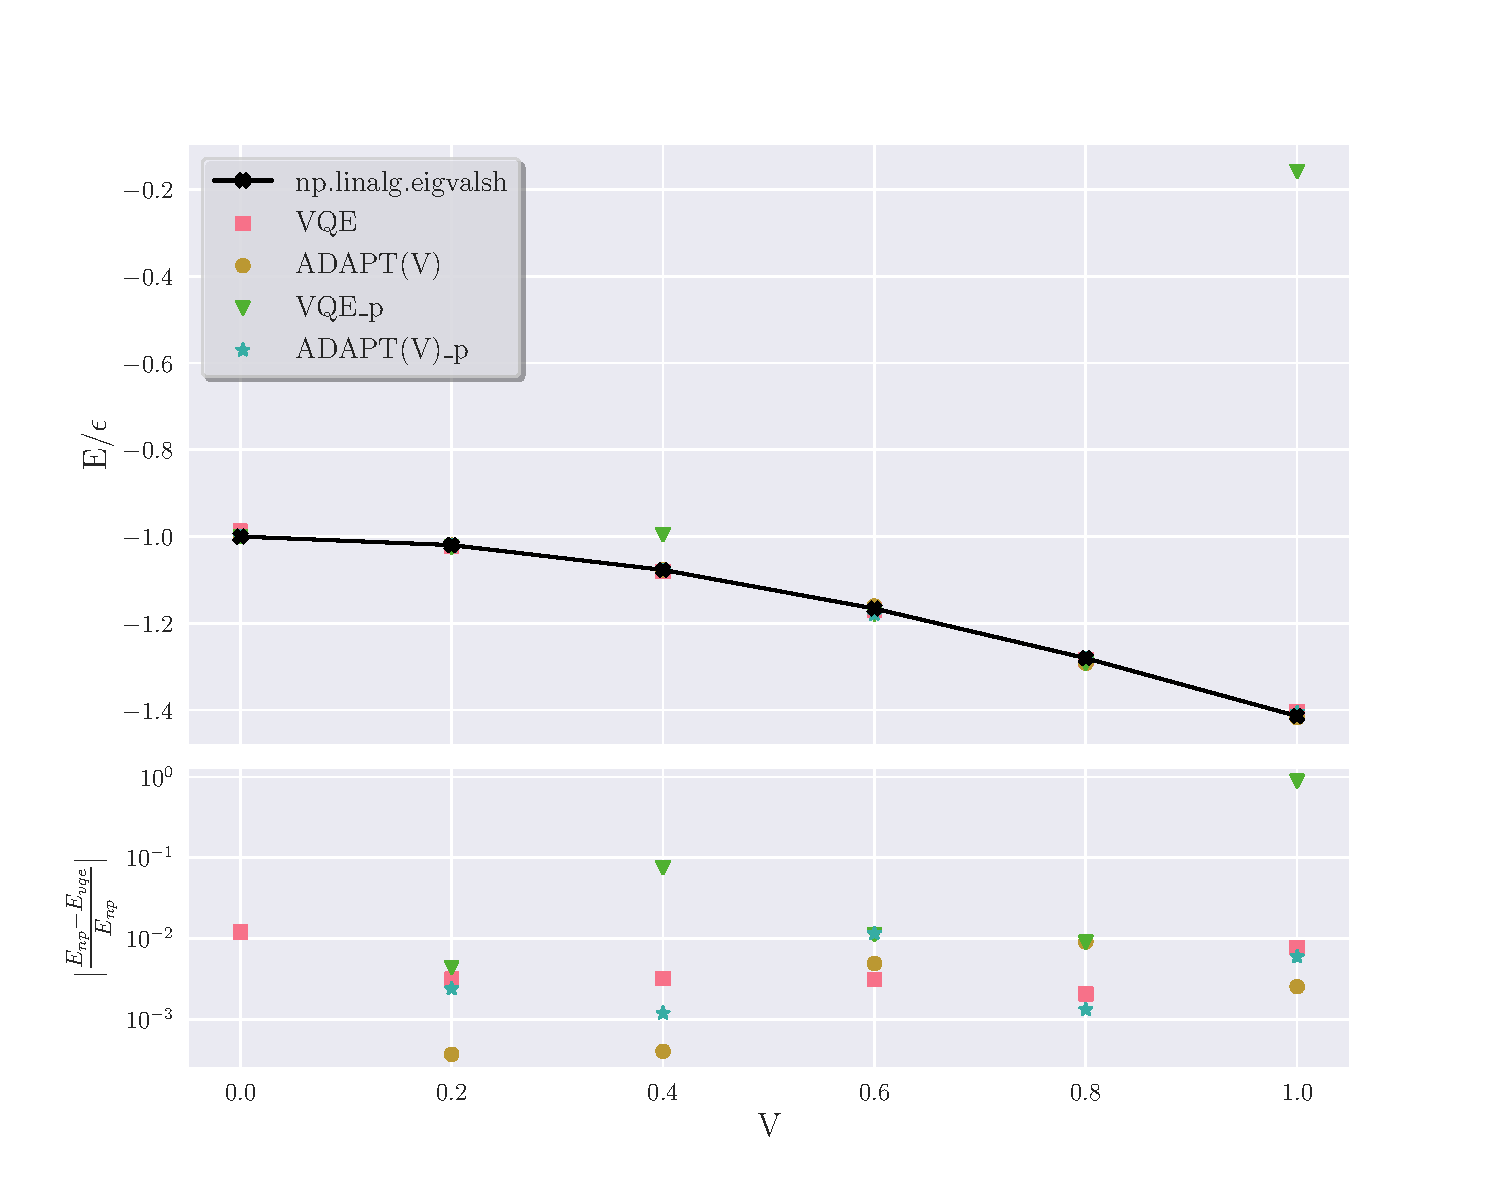
\includegraphics[width=\linewidth]{image/lipkin_result/j1main_True.pdf}
    \caption{The LMG model with $ J=1 $ with \textbf{ideal simulation}, showing the comparison between VQE with $ 1 $ repetition and ADAPT-VQE with the $ V $  pool and $ G $ pool and maximum $ 12 $ ADAPT iterations. The ADAPT-VQE was optimised with the \texttt{COBYLA} method and the normal VQE was with \texttt{Powell}. The label with \textit{\_p} means that the Hamiltonian was mapped using Pauli decomposition, otherwise, Equation~\eqref{eq:rewrite} was used.}
    \label{fig:j1main-noisy}
\end{figure}


\begin{figure}[ht]
    \centering
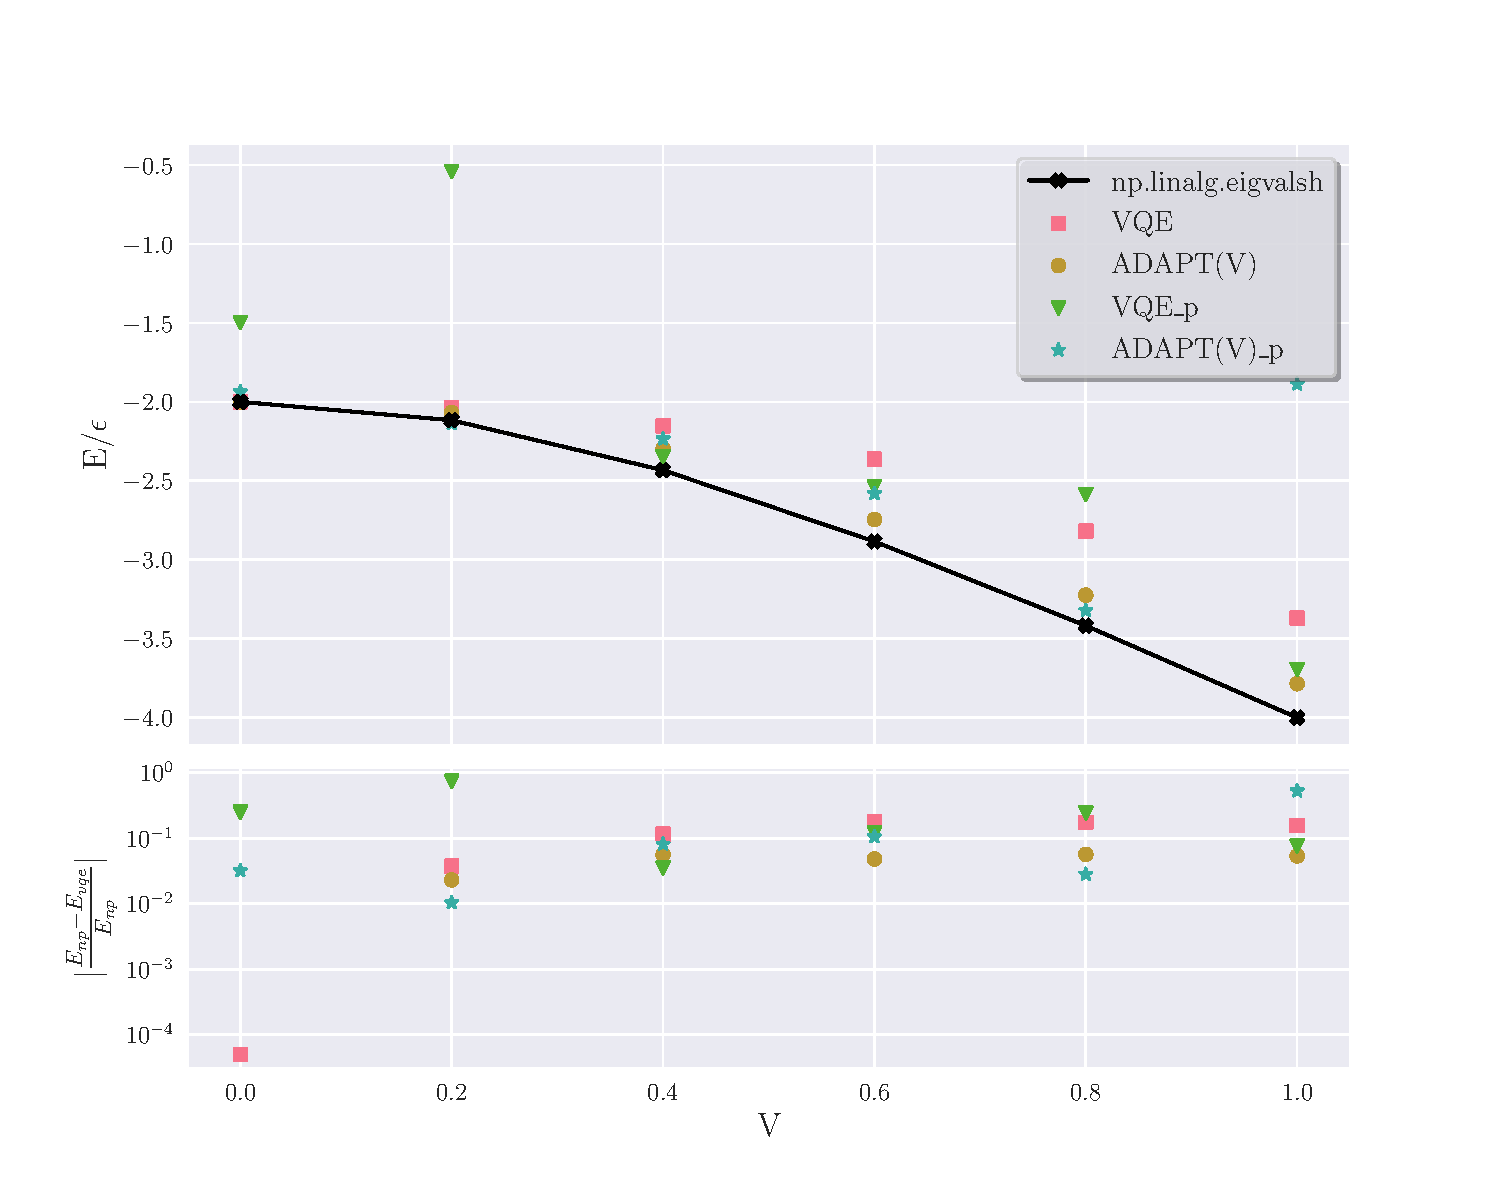
\includegraphics[width=\linewidth]{image/lipkin_result/j2main_True.pdf}
    \caption{The LMG model with $ J=2 $ with \textbf{ideal simulation}, showing the comparison between VQE with $ 1 $ repetition and ADAPT-VQE with the $ G $  pool and $ V $  pool and maximum $ 12 $ ADAPT iterations. The ADAPT-VQE was optimised with the \texttt{COBYLA} method and the normal VQE was with \texttt{Powell}. The label with \textit{\_p} means that the Hamiltonian was mapped using Pauli decomposition, otherwise, Equation~\eqref{eq:rewrite} was used.}
    \label{fig:j2main-noisy}
\end{figure}




\subsection{Circuit Properties}
\label{sub:CircuitProperties}

\begin{table}[ht]
	\centering
	\caption{Table comparison between the fixed-form ansatz and the ADAPT-VQE for both Hamiltonians for the $ J=2 $ case with $ V=1 $ .}
	\label{tab:circuit_prop}

	\begin{tabular}{c c c c c}
		\toprule
		& \textbf{Parameters} &\textbf{Gates} & \textbf{CNOT gates} & \textbf{Energy Function Evaluation} \\
		\midrule

	    Hardware Efficient & 8 & 11 & 3 & 1654\\
		qubit-ADAPT & 12 & 128 & 46 & 846 \\
		Hardware Efficient (Pauli) & 6 & 8 & 2 & 549 \\
		qubit-ADAPT (Pauli) & 12 & 66 & 14 & 801 \\
		\bottomrule
		
	\end{tabular}
\end{table}

Table~\ref{tab:circuit_prop} shows the comparison between the fixed-form ansatzes and the qubit-ADAPTs for the $ J=1 $ case with $ V=1 $. Both qubit-ADAPTs have more parameters and gates, but the number of energy function evaluations is also less for qubit-ADAPT than the HardwareEfficientAnsatz. Pauli-decomposing the Hamiltonian also reduces the resources required to solve the problem. As the hardware efficient ansatz has much fewer gates and CNOT gates, it is expected that there are limitations to the expressibility of the ansatz, hence higher error.

\subsection{Optimisation Methods Comparison}
\label{sub:Optimisers}
In this subsection, we will delve into an analysis of the optimisers used for the VQE and ADAPT-VQE. All optimisers were capped at $ 10000 $ maximum iterations, which is usually never reached. We will choose the best optimisers for both the fixed-form ansatz and the ADAPT-VQE for the main results depending on whether shot noise is present or not.

\subsubsection{Best Optimisers for Fixed-Form Ansatz }%
\label{ssub:BestOptimisersforHW}
This is tested using the qubit Hamiltonian from Equation~\eqref{eq:qubit-hamiltonian-j1-rewrite} and ~\eqref{eq:qubit-hamiltonian-j2-rewrite}  for both the $ J=1 $ and $ J=2 $ cases, which was mapped to a $ 1 $ and $ 2 $ qubits Hamiltonian respectively.

\paragraph{Exact Energy Simulation}
Figure~\ref{fig:opt-fixed-form} shows the comparison between different optimisers for the fixed-form ansatz with \texttt{Rx} and \texttt{Ry} gates without shot noise.

\begin{figure}[ht]
    \centering
    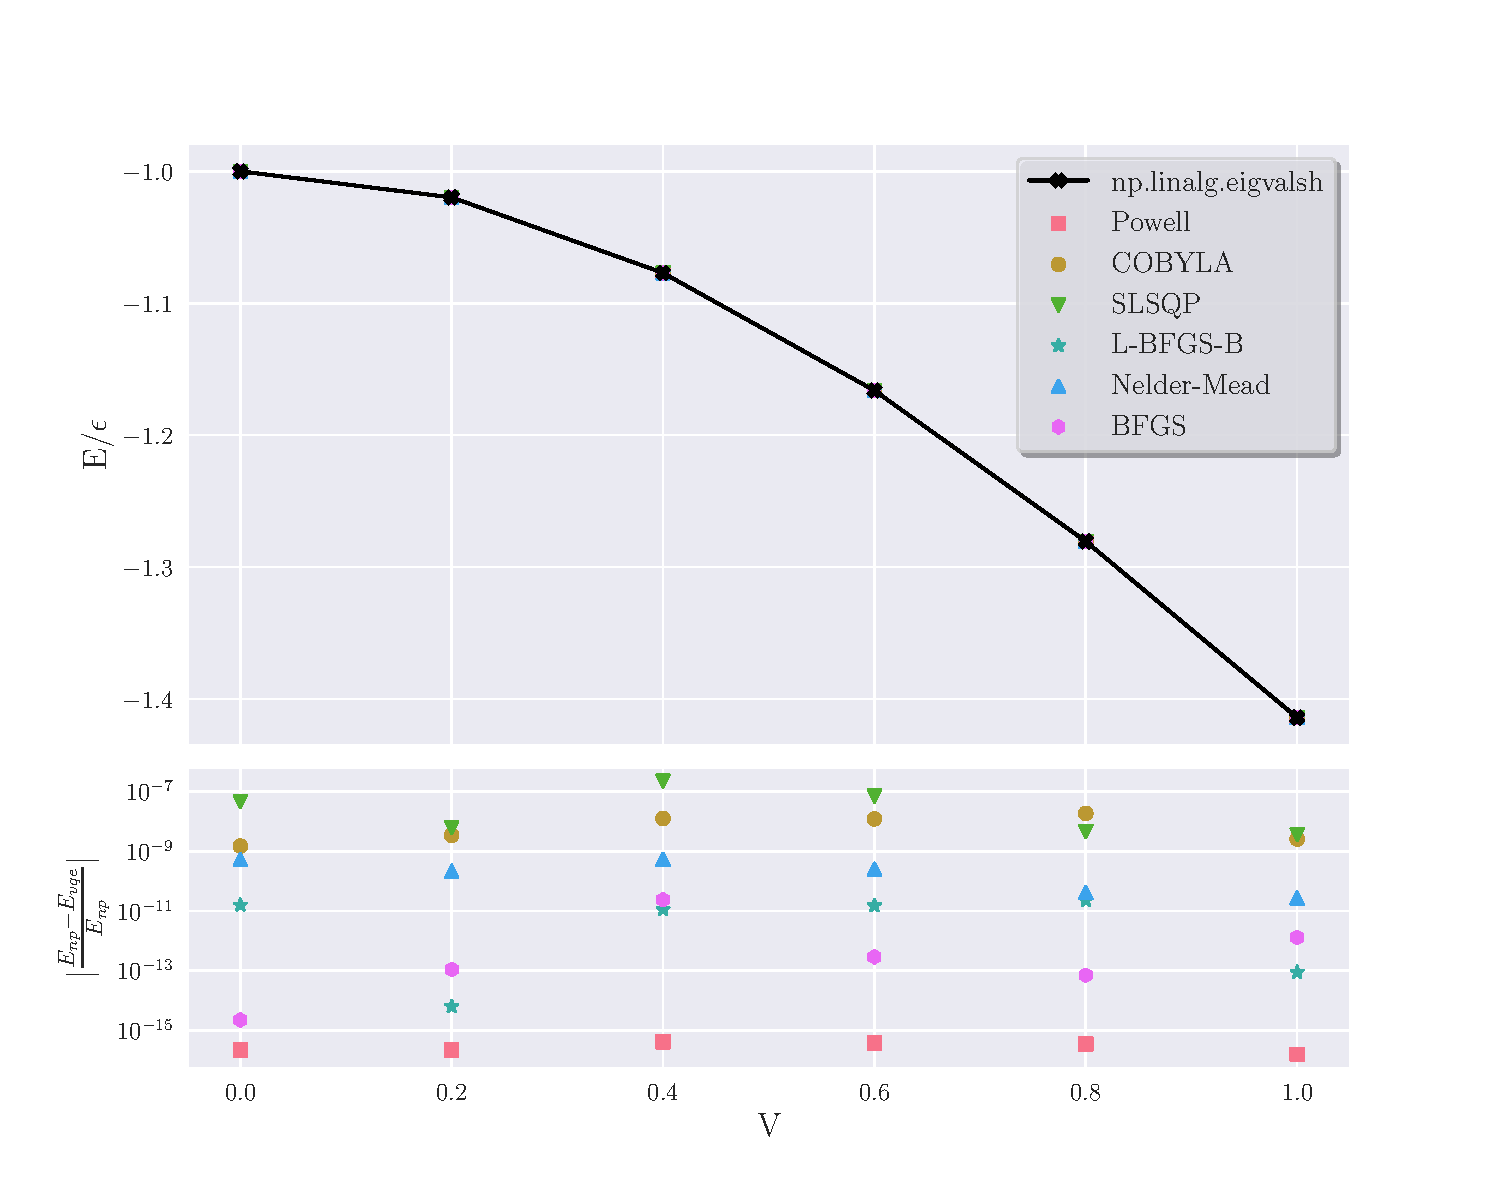
\includegraphics[width=0.45\linewidth]{image/lipkin_result/vqe-opt/cmp_opt_vqe_p_J=1.pdf }
    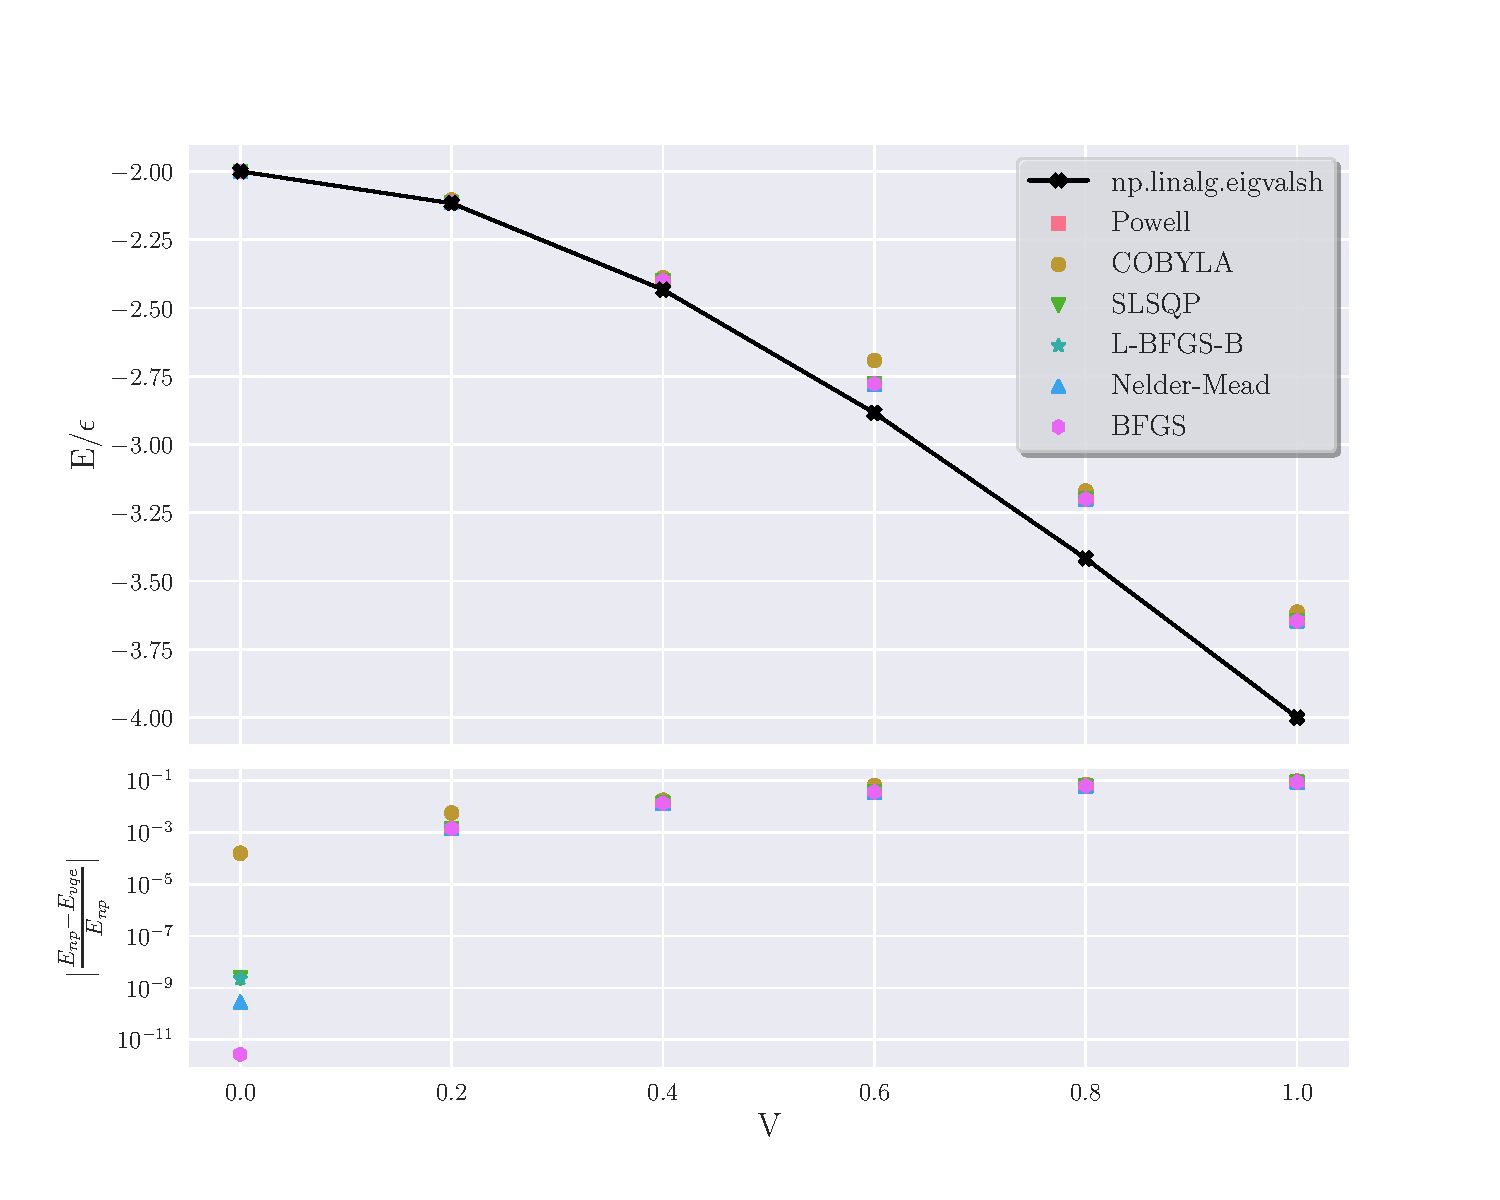
\includegraphics[width=0.45\linewidth]{image/lipkin_result/vqe-opt/cmp_opt_vqe_p_J=2.pdf }
    \caption{Comparison amongst different optimisers for the fixed-form ansatz with \textbf{ exact energy simulation } for $ J=1 $ and $ 2 $  .}
    \label{fig:opt-fixed-form}
\end{figure}

The $ J=1 $ case suggests that Powell is able to achieve the lowest error and the $ J=2 $ case suggests the same, for where the ansatz is expressive enough. Therefore the \texttt{Powell} method will be the choice of optimiser for the fixed-form ansatz for the main exact energy results.

\paragraph{Ideal Simulation}
\begin{figure}[ht]
	\centering
	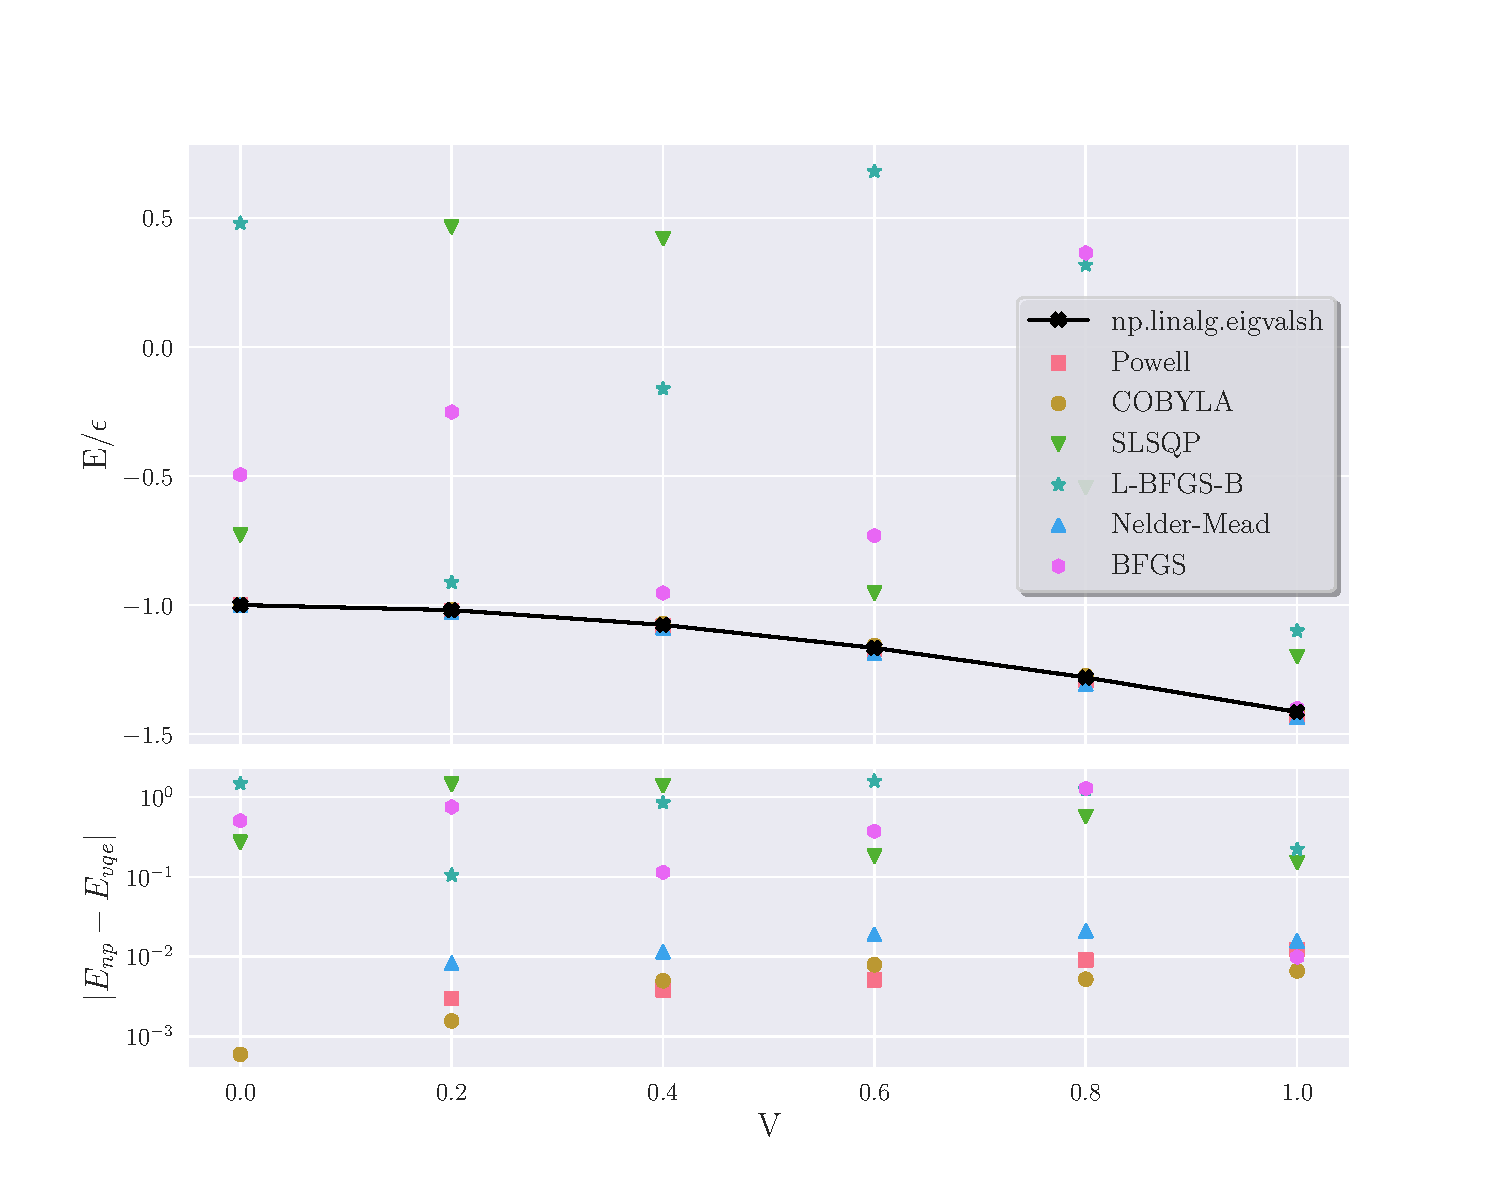
\includegraphics[width=0.45\linewidth]{image/lipkin_result/vqe-opt/cmp_opt_vqe_p_ee100000_J=1.pdf}
	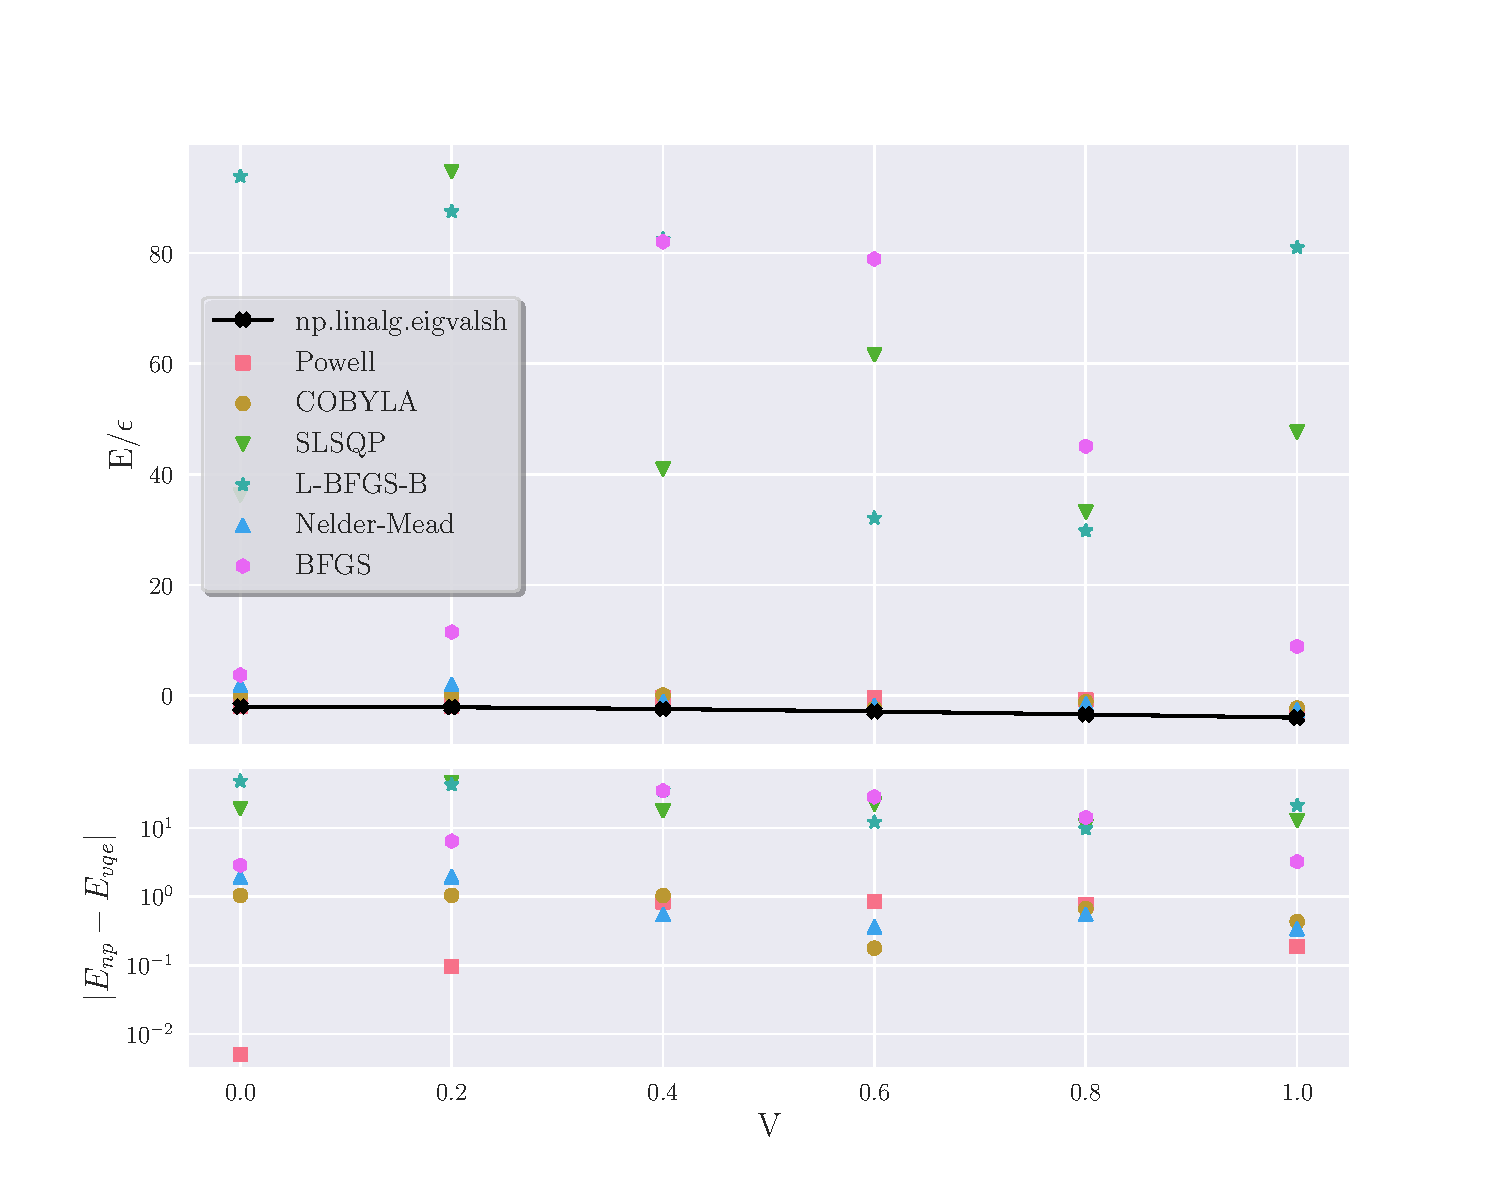
\includegraphics[width=0.45\linewidth]{image/lipkin_result/vqe-opt/cmp_opt_vqe_p_ee100000_J=2.pdf}
	\caption{Comparison amongst different optimisers for the fixed-form ansatz with $ 100000 $ shots for $ J=1$ (left) $J=2 $ (right).}
	\label{fig:Opt-fixed-form-noisy}
\end{figure}

Figure~\ref{fig:Opt-fixed-form-noisy} shows the comparison between different optimisers for the fixed-form ansatz with shot noise. The most robust optimisers for the fixed-form ansatz with shot noise are \texttt{COBYLA} and \texttt{Powell}. The \texttt{Nelder-Mead} method produced reasonable results for some interaction strength but struggles at large interaction strength. Since Powell has better performance for both cases, it will be the choice of optimiser for the main results.

\subsubsection{Best Optimisers for the qubit-ADAPT-VQE}%
\label{ssub:BestOptimisersforADAPT}

\paragraph{Exact Energy Simulation}
Figure~\ref{fig:OptAdapt} shows the comparison between different optimisers for the ADAPT-VQE without shot noise. We see that BFGS and L-BFGS-B were able to achieve the lowest energy errors.
\begin{figure}[ht]
	\centering
	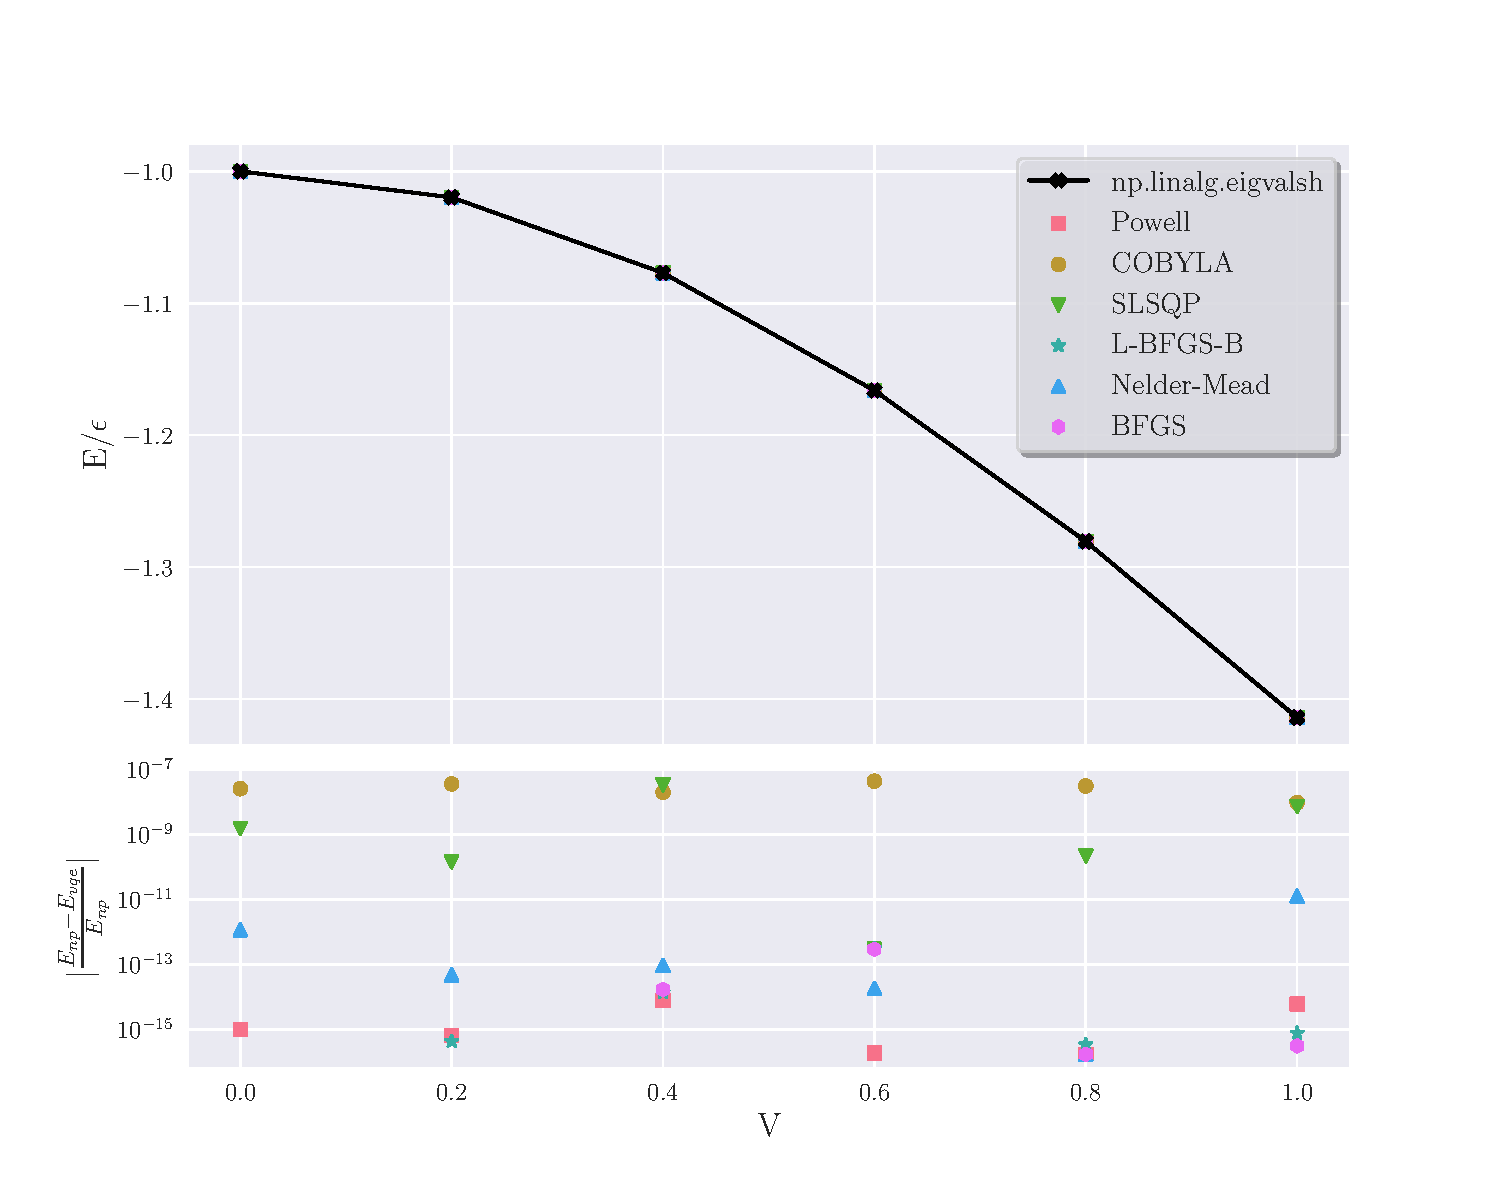
\includegraphics[width=0.47\linewidth]{image/lipkin_result/adapt-opt/cmp_opt_adapt_p_J=1.pdf}
	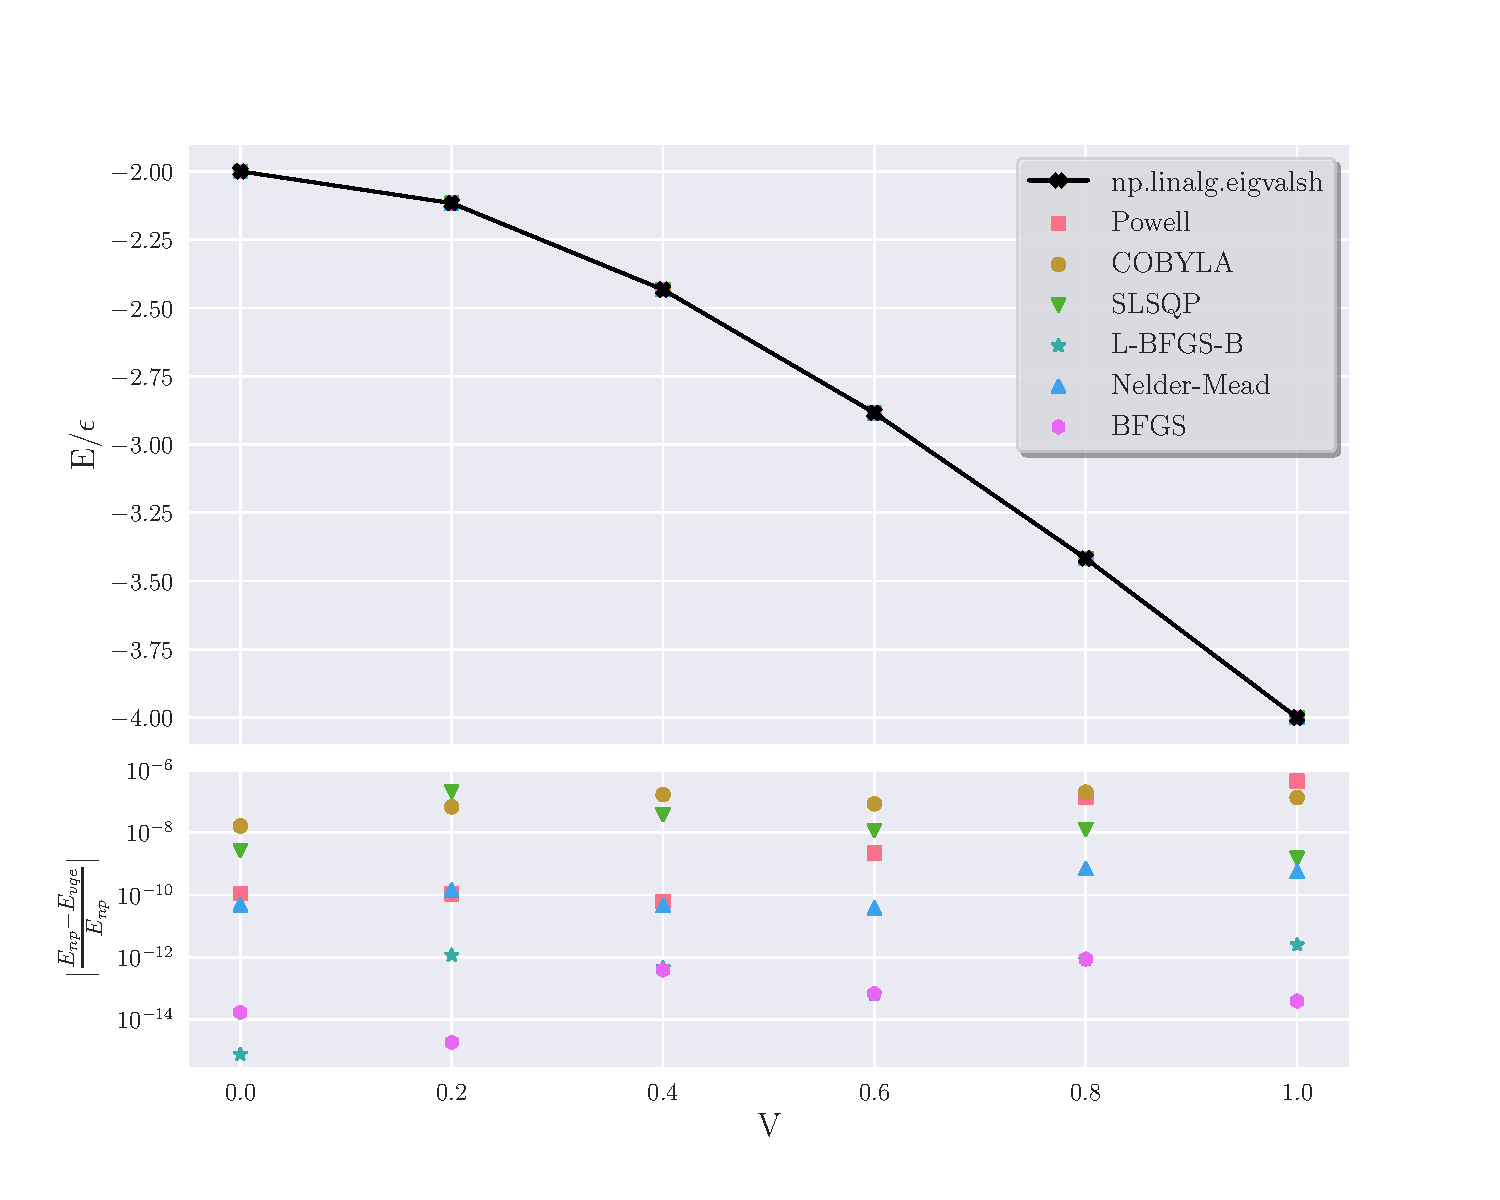
\includegraphics[width=0.47\linewidth]{image/lipkin_result/adapt-opt/cmp_opt_adapt_p_J=2.pdf}
	\caption{Comparison amongst different optimisers for the ADAPT-VQE without shot noise for $ J=1 $ (top) and $ J=2 $ (bottom).}
	\label{fig:OptAdapt}
\end{figure}

\begin{figure}[ht]
	\centering
	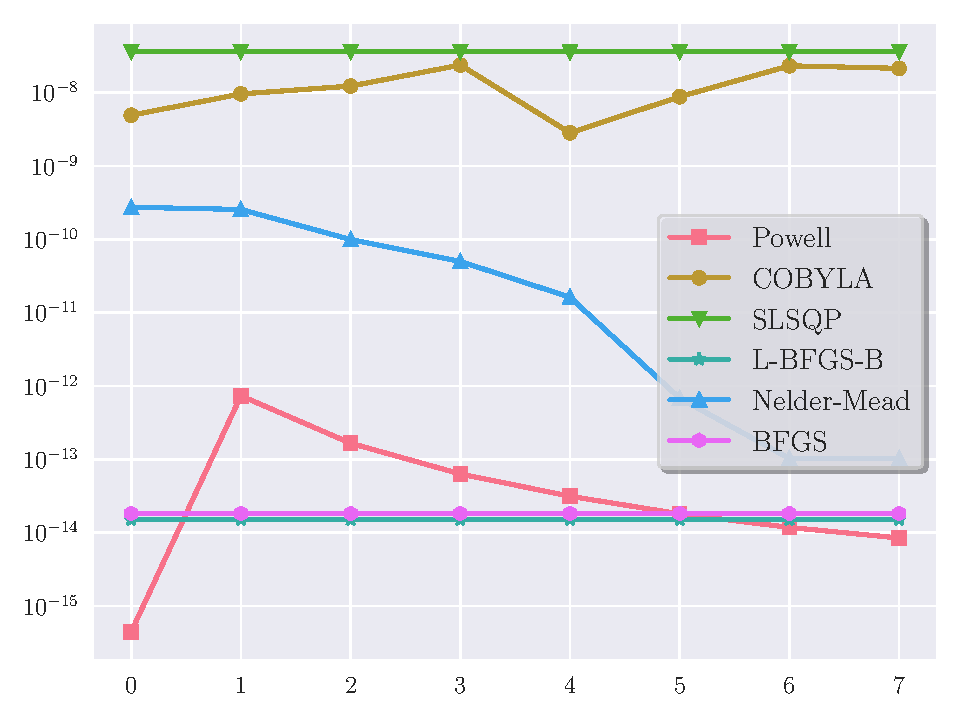
\includegraphics[width=0.47\linewidth]{image/lipkin_result/onlyneed1iter.pdf}
	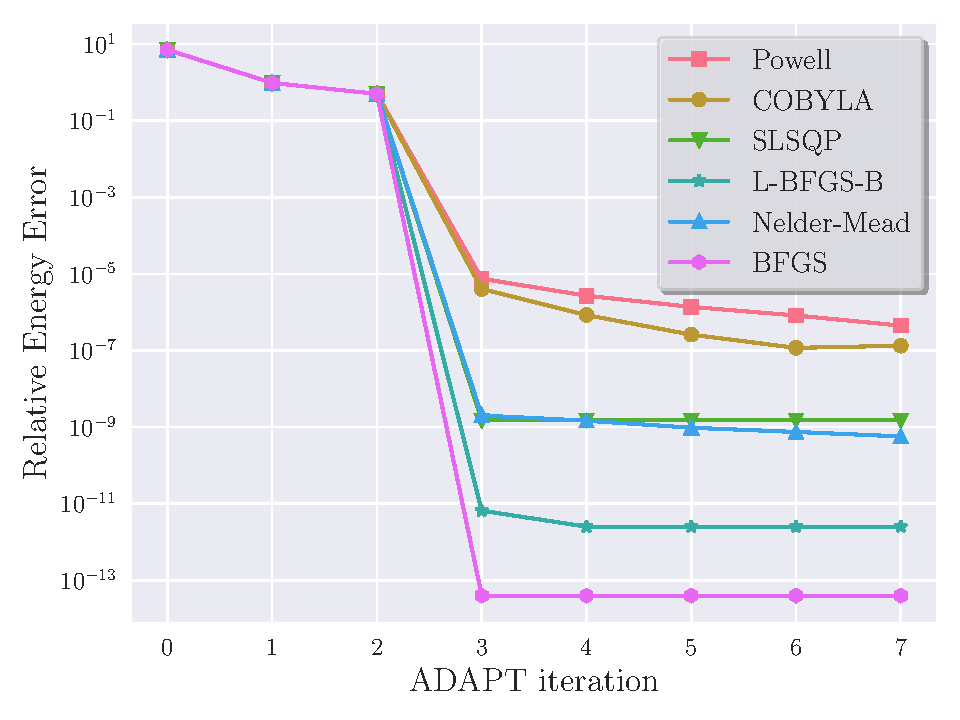
\includegraphics[width=0.47\linewidth]{image/lipkin_result/onlyneed3iter.pdf}
	\caption{Comparison amongst different optimisers for the ADAPT-VQE without shot noise for $ J=1 $ and $ J=2 $.}
	\label{fig:onlyneed1iter}
\end{figure}

As seen in Figure~\ref{fig:onlyneed1iter}, all the optimisers were able to achieve high accuracy with just one iteration for the $ J=1 $ case, and for the $ J=2 $ case it took only $ 3 $ iterations for all ADAPT to converge regardless of the choice of optimisers.

\paragraph{ideal Simulation}

As it turned out, the best optimisers that are robust against shot noise are different from those without shot noise. Whilst we see that all optimisation methods converge to different accuracies for the case without shot noise, some optimisers have shown to be more robust against shot noise. Noticeably, Nelder-Mead takes much longer to converge compared to other methods. 


\begin{table}[ht]
    \centering
    \caption{Optimisersation Results for $ J=1 $ and $ v = 1 $ }
    \label{tab:label}
    \begin{tabular}{c c c c}
	\toprule
	& \textbf{Function Calls} & \textbf{Run Time (s)} & \textbf{Relative Error} \\
	\midrule
	\texttt{COBYLA} & 399 & 2.481 & 0.00268 \\
	\texttt{Powell} & 2475 & 10.849 & 0.01498\\
	\texttt{SQSLP} & 172 & 0.871 & 0.3144 \\
	\texttt{BFGS} & 1160 & 3.749 & 0.286 \\
	\texttt{L-BFGS-B} & 1145 & 4.190 & 0.301  \\
	\texttt{Nelder-Mead} & 219625 & 749.491 & 0.263\\
	\bottomrule
    \end{tabular}
\end{table}

Even for $ N = 10^4 $ shots, most of the optimisers struggle to converge to the correct values. Since only \texttt{COBYLA} and \texttt{Powell} are able to converge to the correct values, they will be the choice of optimisers for the ADAPT-VQE for the main results. Interestingly, they seem to converge to the same values as shown in Figure~\ref{fig:optcmpj1}. 
\begin{figure}[ht]
	\centering
	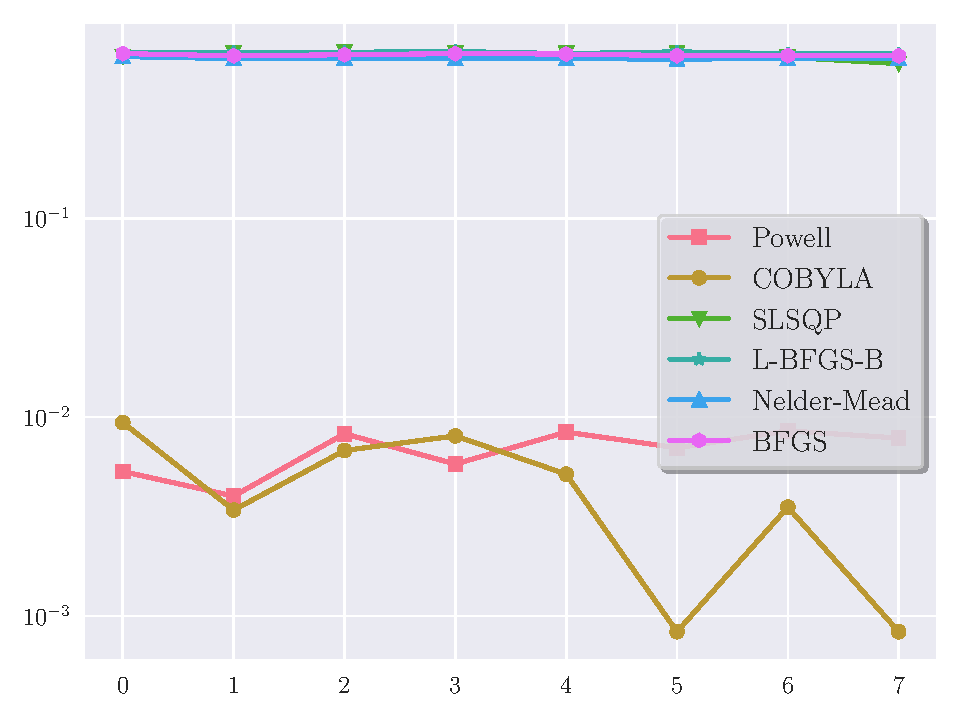
\includegraphics[width=0.45\linewidth]{image/lipkin_result/whynotothersv=0.4.pdf}
	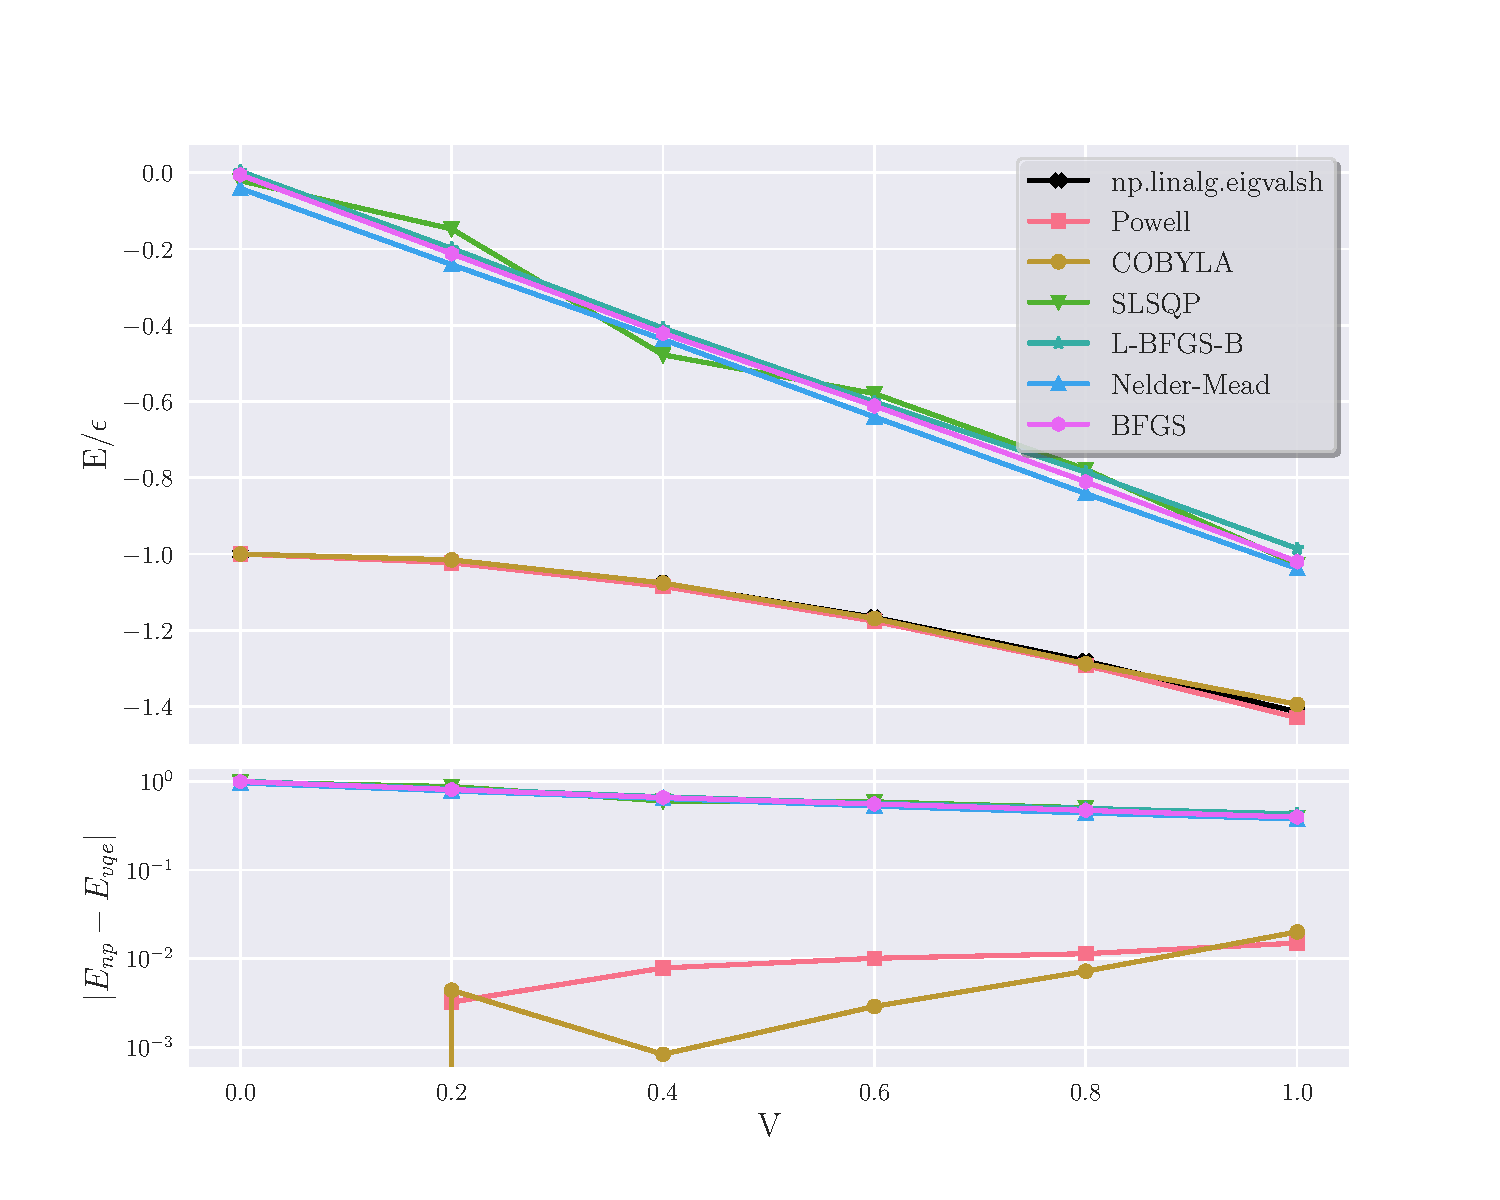
\includegraphics[width=0.45\linewidth]{image/lipkin_result/whynotothers10e4.pdf}	
	\caption{(Left) Comparison amongst different optimisers for the ADAPT-VQE, relative error per ADAPT iterations for $ 8 $ iterations with $ 10e_4 $ shots for $ J=1 $ at $V=0.4$. (Right) Energy plot for different optimisers for different values of $V$.}
	\label{fig:optcmpj1}
\end{figure}

To rule out the possibility that the optimisers which failed to converge were stuck in a local minimum, we could plot the energy landscape for the $ J=1 $ case since there is only one qubit. The energy landscape is shown in Figure~\ref{fig:energy_landscape}. In this case, we only need $ \text{Rx}(\theta) $ and $ \text{Ry}(\phi) $ to span the entire Hilbert space, and the state is then $ R_x(\theta) R_y(\phi)\ket{0}$. The energy landscape shows that there is only a single minimum (within a period), which is the one we are interested in. It is simply a result of the shot noise that the optimisers do not converge properly, which agrees with  Figure~\ref{fig:OptAdapt}, as all the optimisers were able to converge after $ 1 $ iteration.

\begin{figure}[ht]
	\centering
	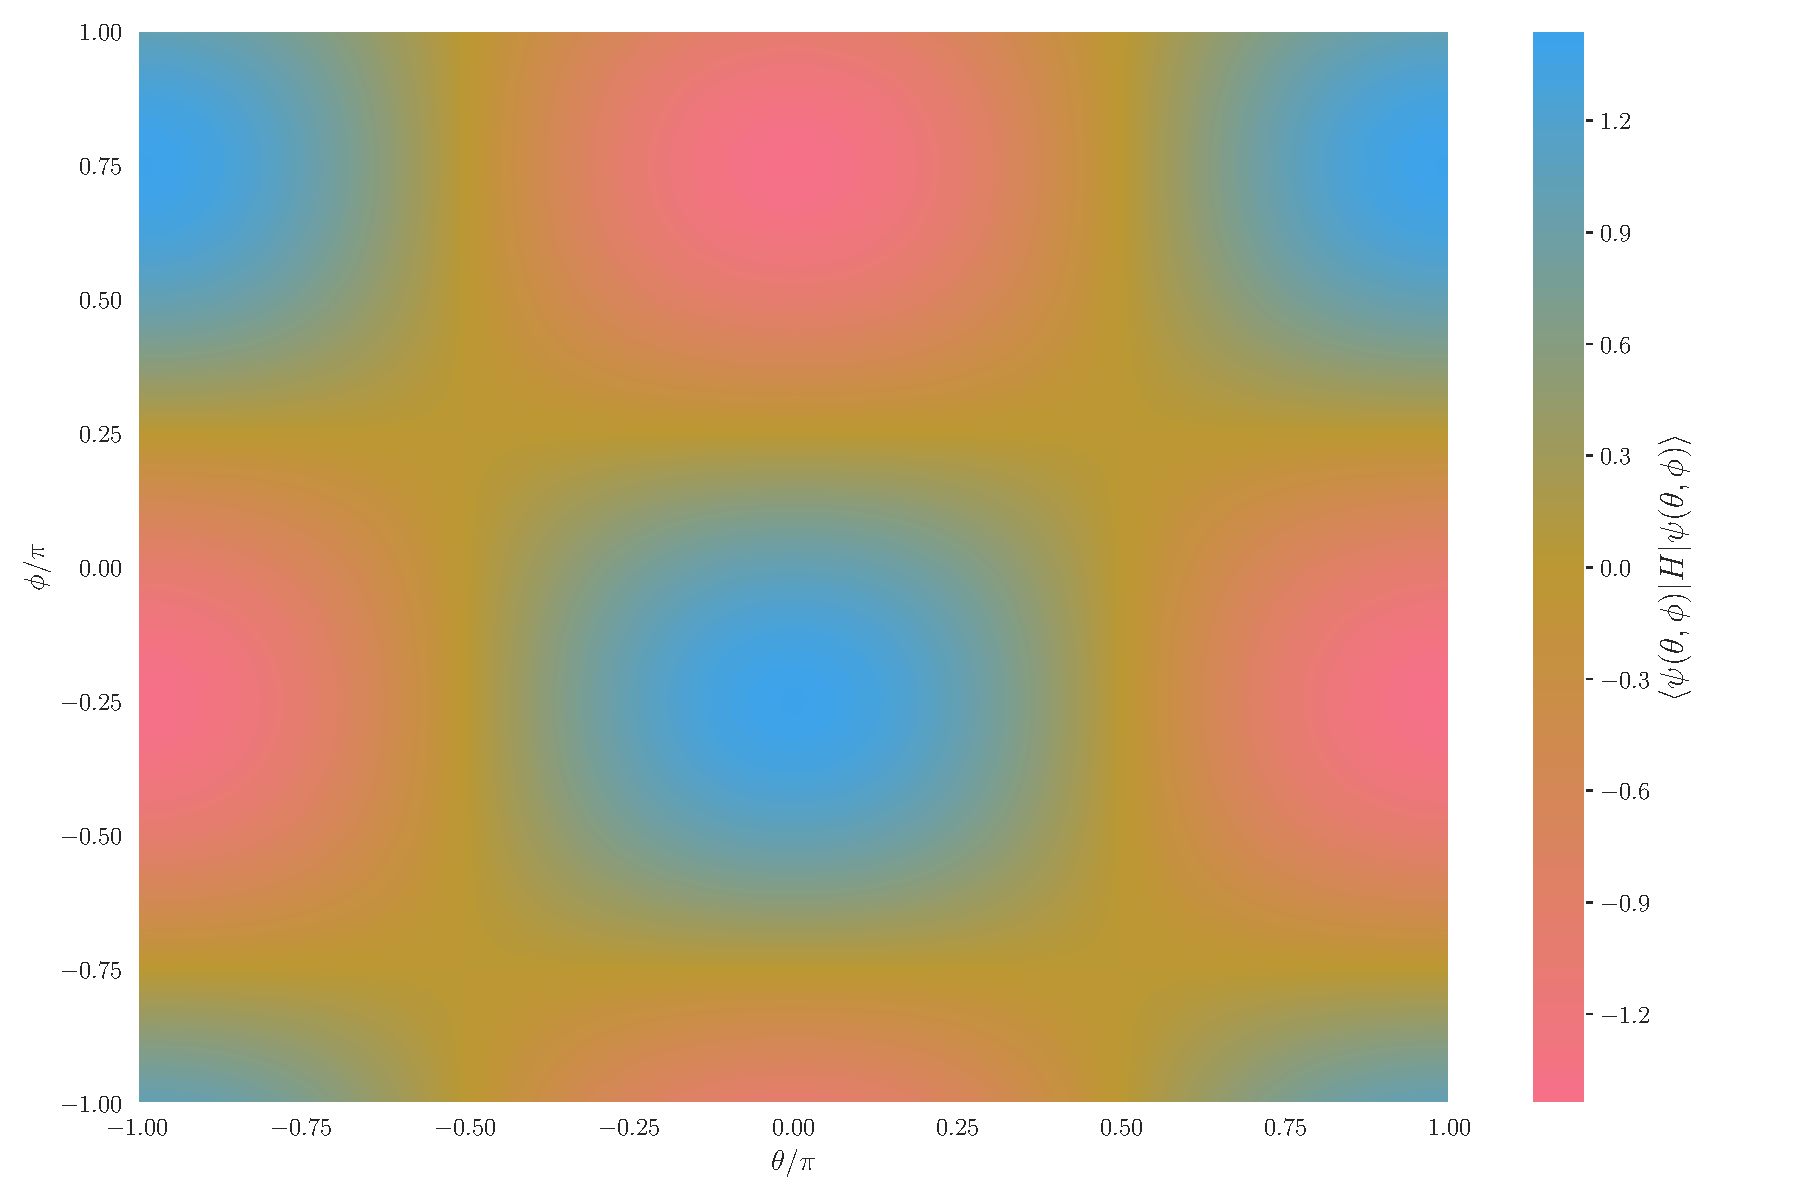
\includegraphics[width=\linewidth]{image/lipkin_result/energy_landscape.pdf}
	\caption{Energy landscape for $J=1$ with $V=1$. } 
	\label{fig:energy_landscape}
\end{figure}



\section{Pairing Model}
\label{sec:pairing_result}
In this section, we show the results of the Pairing model with 4 doubly degenerate states and $ 4 $ particles for both the exact energy and ideal simulation. There are $ 18 $ terms in the qubit Hamiltonian for the pairing model. Therefore the expected error for the pairing model is $ 0.013 $. We have chosen $ \xi = 1 $ and the energy plotted is normalised by $ \xi $ and is hence unitless.

\begin{figure}[ht]
    \centering
    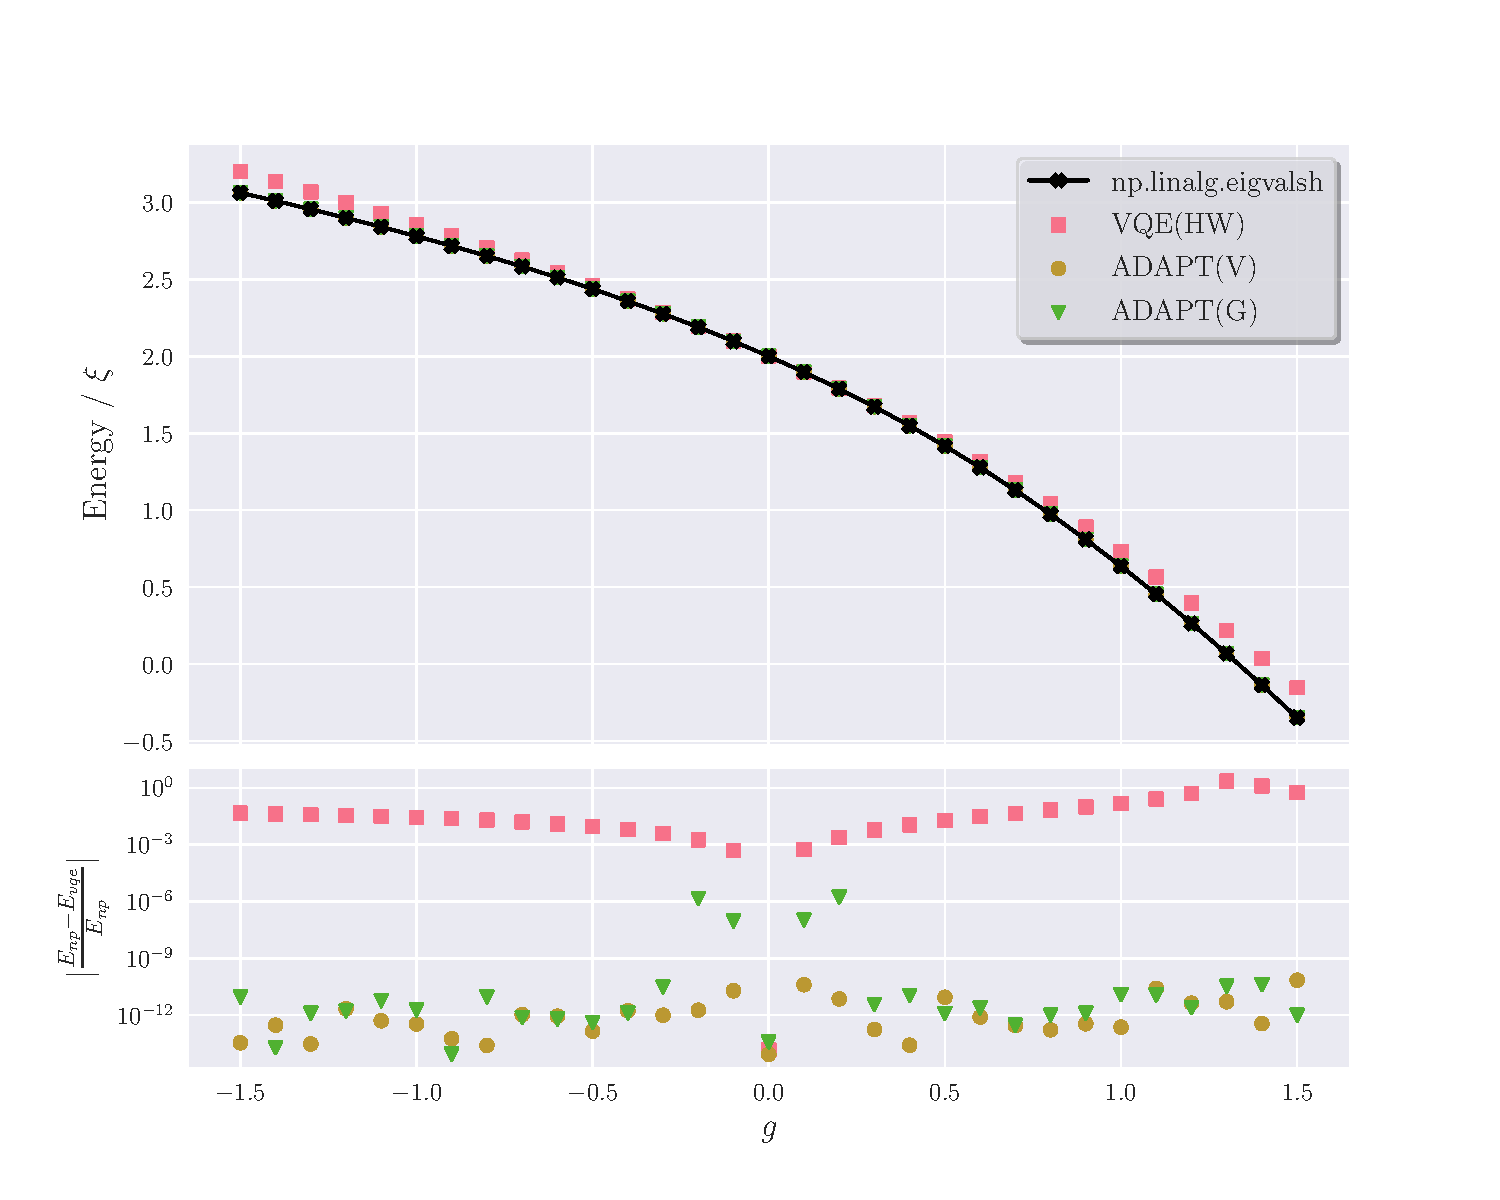
\includegraphics[width=\linewidth]{image/pairing_result/no_shot_noise/pairing-main-result.pdf}
    \caption{\textbf{Exact energy simulation} for the pairing model with \texttt{BFGS} optimiser for both the ADAPT-VQE and the VQE for a maximum of $ 8 $ iterations and $ g \in[-1.5,1.5] $. The hardware efficient ansatz with 2 repetitions was used for the VQE.}
    \label{fig:small-main}
\end{figure}

We first look at the results for $ g \in [-1.5, 1.5] $ for the ADAPT-VQE with both the $ V $ pool and the $ G $ pool, as well as the hardware efficient ansatz. As we can see from Figure~\ref{fig:small-main}, when exact energy is calculated, the ADAPT-VQEs with both pools were able to converge to the exact energy diagonalisation n with errors of orders of $ 10^{-9} $ for $ g \in [-1.5, 1,5] $ for only $ 8 $ maximum iterations. The $G$ pool performd slightly worse (with error $ \sim \mathcal{O}(10^{-6}) $ ) for values close to $ 0 $. The hardware efficient ansatz was not able to obtain the same level of accuracies as the ADAPT-VQE, but the relative error was consistent for most of the values of $ g $ in orders of $ 10^{-2} $, with the exception of $ g = 0$ where the Hamiltonian given by Equation~\eqref{eq:pairing-mat} is diagonal, which the hardware efficient ansatz was able to represent exactly.

\begin{figure}[ht]
    \centering
    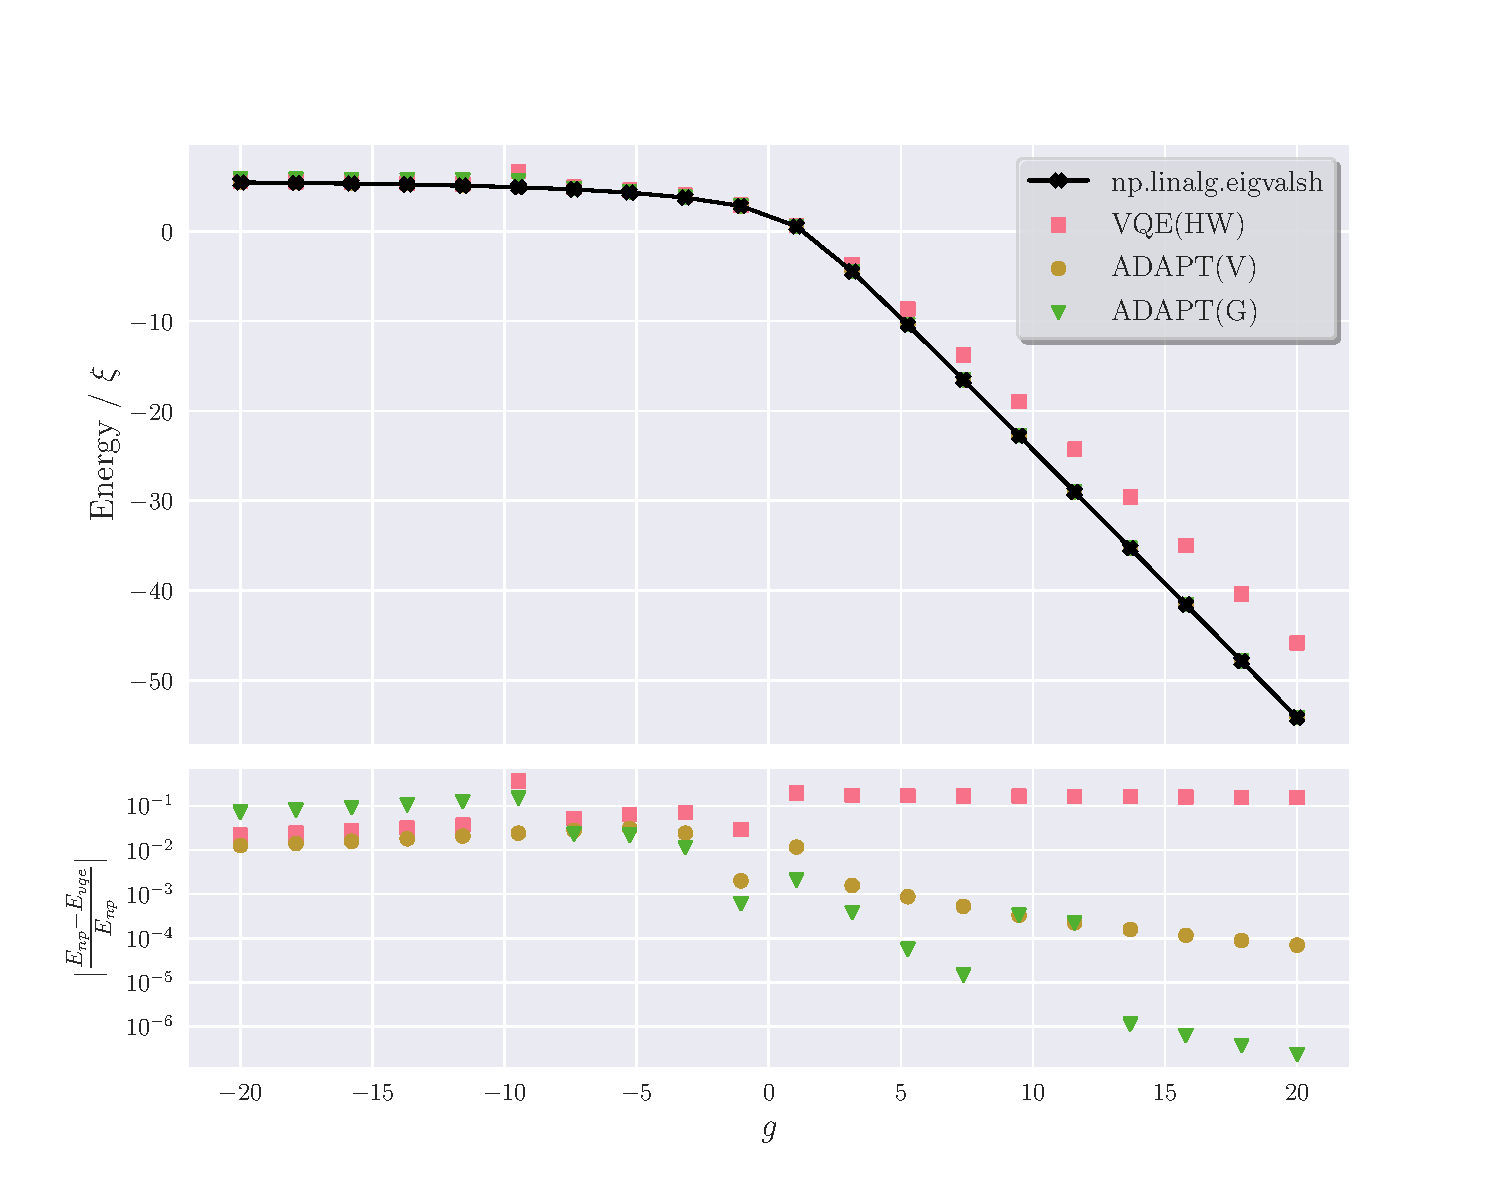
\includegraphics[width=\linewidth]{image/pairing_result/no_shot_noise/sameparams-big.pdf}
    \caption{\textbf{Exact energy simulation} for the pairing model with \texttt{BFGS} optimiser for both the ADAPT and the normal VQE for a maximum of $ 6 $ iterations and $ g \in[-20,20] $. The HW ansatz with 2 repetitions was used for the VQE.}
    \label{fig:big-main}
\end{figure}


We ran the exact energy simulation again for $ g \in [-20,20] $, as shown in Figure~\ref{fig:big-main}. The number of maximum iterations was set to $ 6 $ to match the parameter in the hardware efficient ansatz with $ 2 $ repetitions. For values of $ g \in [-20,0] $, the ADAPT-VQEs performed similarly to the VQE, with an error between $ 10^{-2} $ to $ 10^{-1} $. However, for large pairing strength $ g $, the ADAPT-VQEs perform much much better than the VQE. The reason why the ADAPT-VQEs do not perform as well for the negative region of $ g $ could be due to the fact that $ 6 $ maximum iterations were not enough for the ADAPT-VQE to converge. Another point worth noting is that the bottom plot in Figure~\ref{fig:big-main} is the relative error. As the energy increases, the energy increases in magnitude, and the relative error takes account into the fact of the changing magnitude of the energy, making it a better indicator than the absolute error for algorithmic performance. 

\begin{figure}[ht]
    \centering
    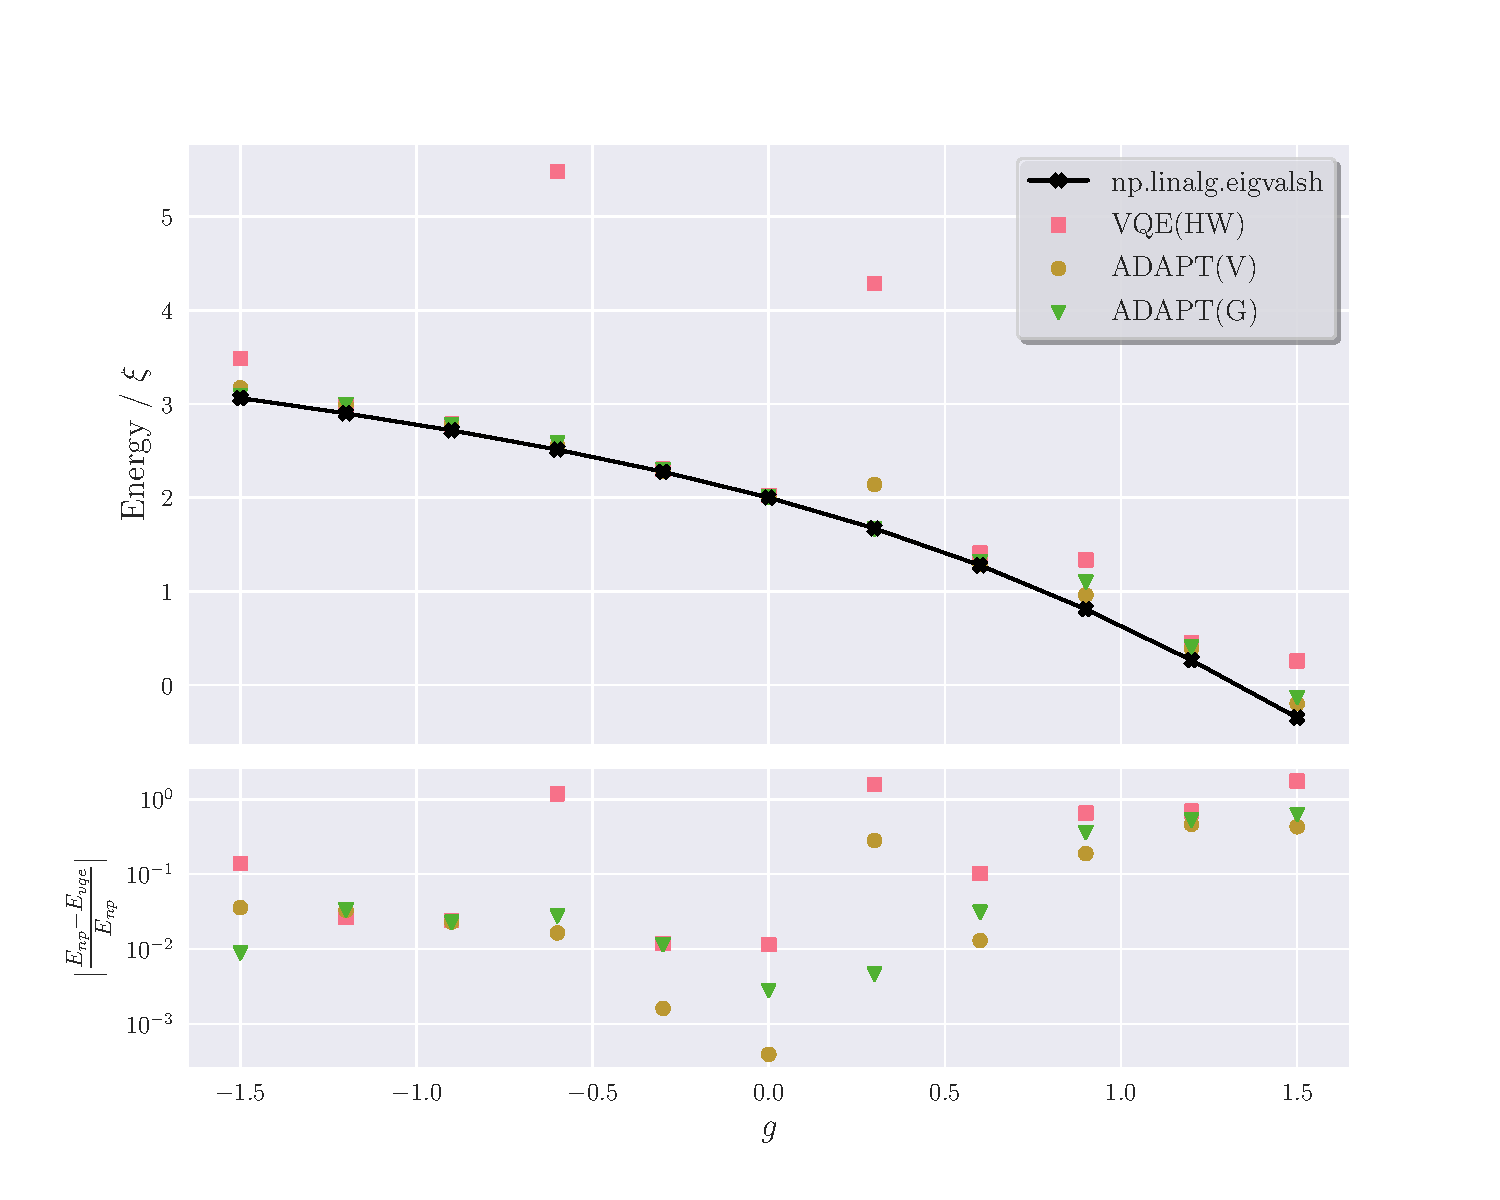
\includegraphics[width=\linewidth]{image/pairing_result/ideal simulation/noisy-16-sm.pdf}
    \caption{\textbf{Ideal Simulation} for the pairing model with \texttt{COBYLA} method for the ADAPT-VQEs and \texttt{Powell} for the VQE for a maximum of $ 16 $ iterations for $ g \in[-1.5,1.5] $. The hardware efficient ansatz with 2 repetitions is used for the VQE.}
	\label{fig:small-main-noisy}
\end{figure}
\begin{figure}[ht]
    \centering
    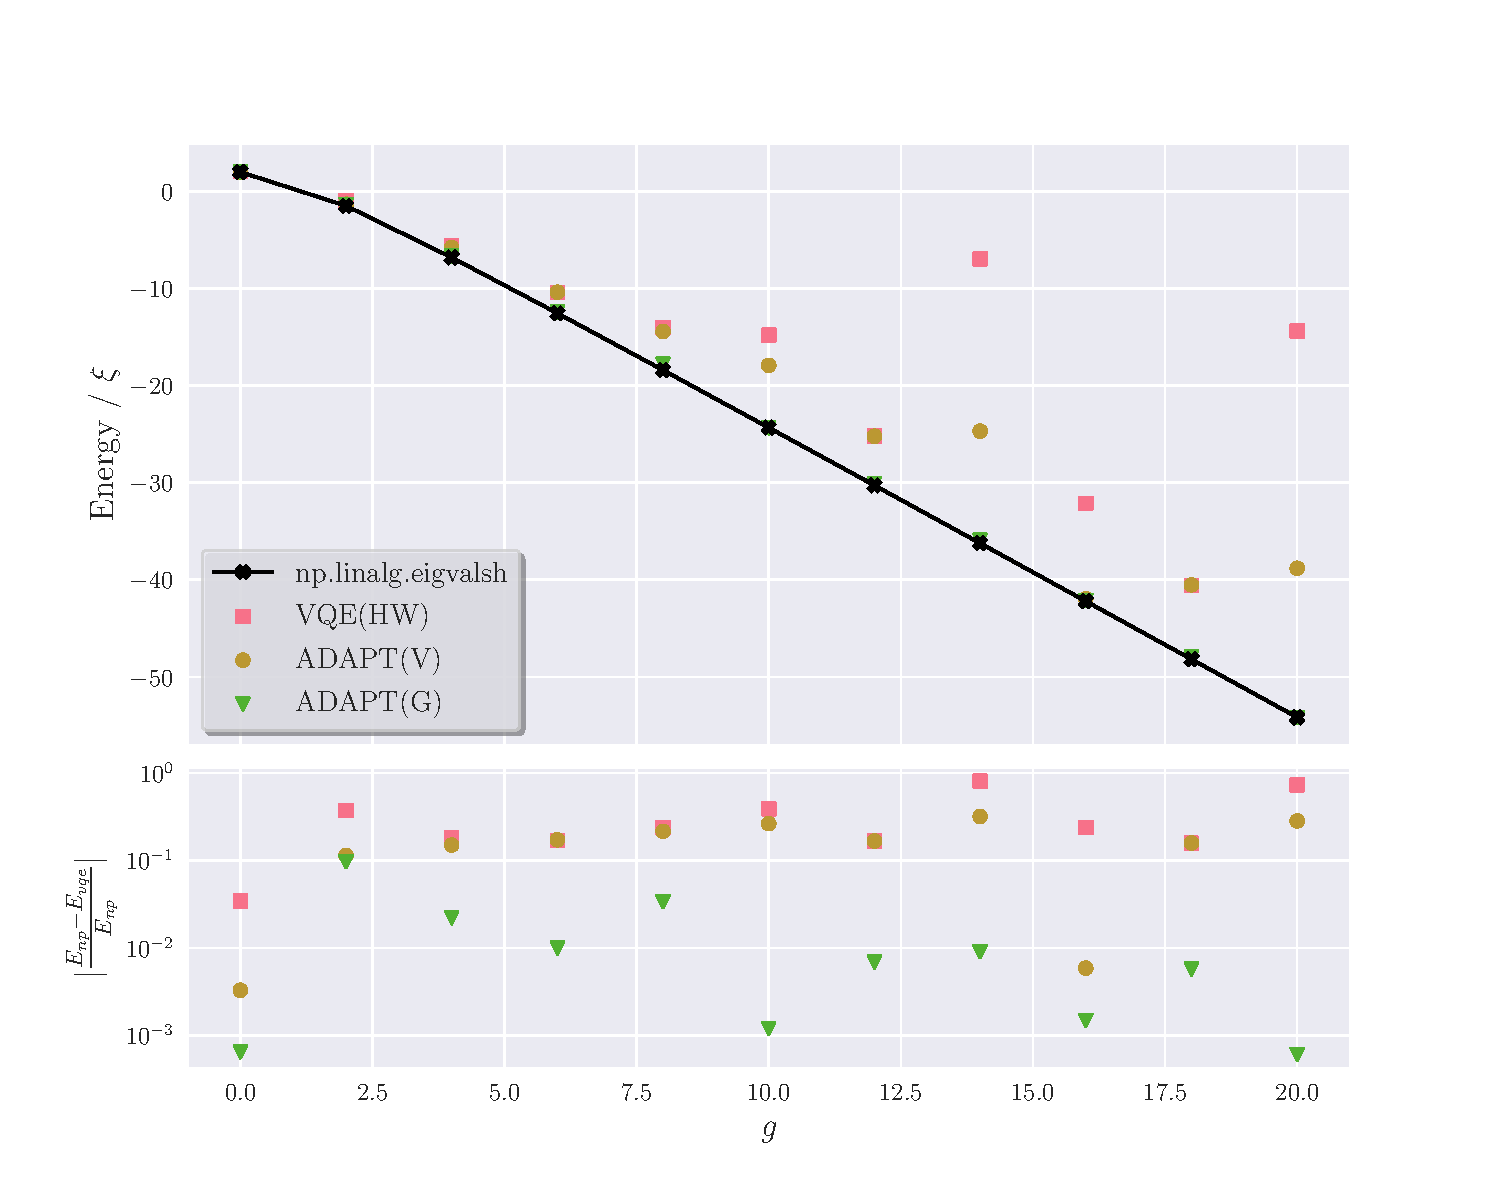
\includegraphics[width=\linewidth]{image/pairing_result/ideal simulation/noisy-16-big.pdf}
    \caption{\textbf{Ideal Simulation} for the pairing model with \texttt{COBYLA} method for the ADAPT-VQE and \texttt{Powell} for the VQE for a maximum of $ 16 $ iterations for $ g \in[0,20] $} 
    \label{fig:big-main-noisy}
\end{figure}

Figure~\ref{fig:small-main-noisy} shows the results for the ideal simulation of the pairing model. We expected that by including shot noise the ADAPT-VQEs would require more iterations to converge, hence the maximum iteration was increased to $ 16 $.

For $ g \in [-1.5, 1.5]$, the results produced with both ADAPT-VQEs and the VQE performed similarly in terms of accuracies. However, the ADAPT-VQEs were more consistent in convergence to the ground state while for many points the VQE did not manage to converge. This is aligned with the analysis we performed earlier for the LMG model for Figures~\ref{fig:j2main-nsn} and~\ref{fig:j2main-noisy} where for some points the VQE with hardware efficient ansatz failed to converge. 

Results for ideal simulation for $ g \in [0,20] $ are presented in Figure~\ref{fig:big-main-noisy}. This is the only time we observed a difference in the performance of the pools. We observed similar results in Figure~\ref{fig:big-main} but fewer iterations were allowed and the differences were not as clear. The $ G $  pool consistently outperformed the $ V $  pool in the interval $ g \in [0,20] $, with errors within orders of $ 10^{-2} $, while the V pool performed similarly to the VQE with hardware efficient ansatz. Looking into the details we included $ 2 $ ADAPT iteration graphs shown in Figure~\ref{fig:8-16-iter} for $ g=8 $ and $ g=16 $ respectively. In both cases, the $ G $ pool found the operators which allowed it to converge after just a couple of iterations, whereas for the $ V $ pool, appending new operators did not improve the energy. For the $ g=8 $ case, the $ V $ pool did not converge at all and for the $ g=16 $ case, the energy started to decrease at around $ 11 $ iterations, much later than the $ G $ pool. Looking at the structure of the pools as presented in equations~\eqref{eq:gpool} and ~\eqref{eq:vpool}, we could see that the operators in the $ G $ pool have a localised structure but it is unclear what was the cause of the difference in performance.

\begin{figure}[ht]
    \centering
    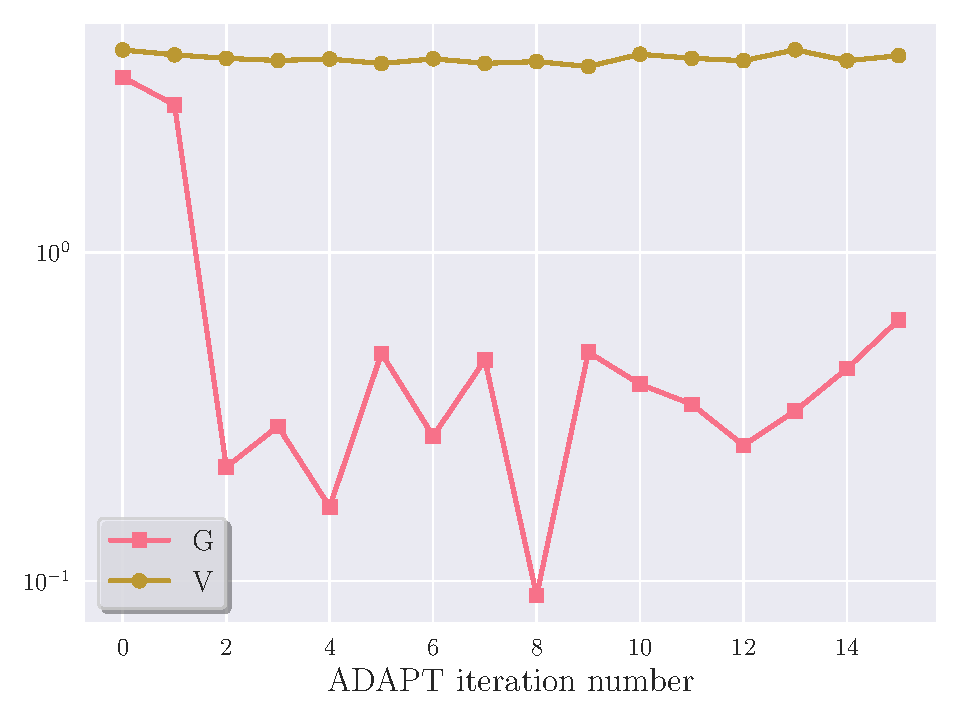
\includegraphics[width=0.45\linewidth]{image/pairing_result/ideal simulation/g8.pdf}
    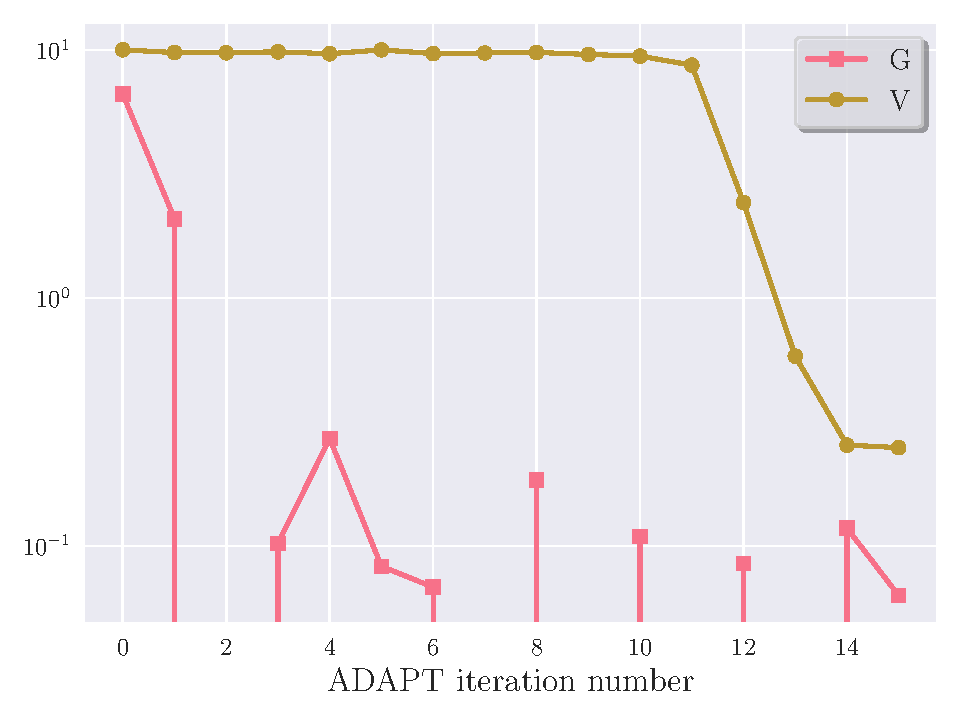
\includegraphics[width=0.45\linewidth]{image/pairing_result/ideal simulation/g=16adaptiter.pdf}
    \caption{ADAPT-VQE error at every iteration for the pairing model using \texttt{COBYLA} optimiser for $ g=16 $ (left) and $ g=18 $ (right).}
    \label{fig:8-16-iter}
\end{figure}


\section{Deuteron Model}
\label{sec:deuteron_result}


In this section, we present both the exact energy simulation and ideal simulation results for the deuteron model for different numbers of basis dimensions $ N $. We compare our results to the numerical diagonalisation using $ numpy.linalg.eigvalsh$. For the deuteron model with $ N=n $, the number of qubits required is $ \lceil \log_2( n ) \rceil$. Unlike the other models we have simulated, the qubit Hamiltonians of the deuteron model will have a different number of terms for different values of $ N $, and the expected error depends on $ N $ as well. This is an interesting case to include as we can easily compare the performance for different numbers of qubits for the same system. 
The numbers of terms in the Hamiltonian are $ 8,20$ and $48 $ for the $ 2,3$ and $4$ qubit cases respectively, so the expected error for these cases should be $ \mathcal{O}(10^{-2}) $.

\subsection{Exact Energy Simulation}
We first look at the results for $ N \in [2,32] $ for the exact energy simulation. 

\begin{figure}[ht]
    \centering
    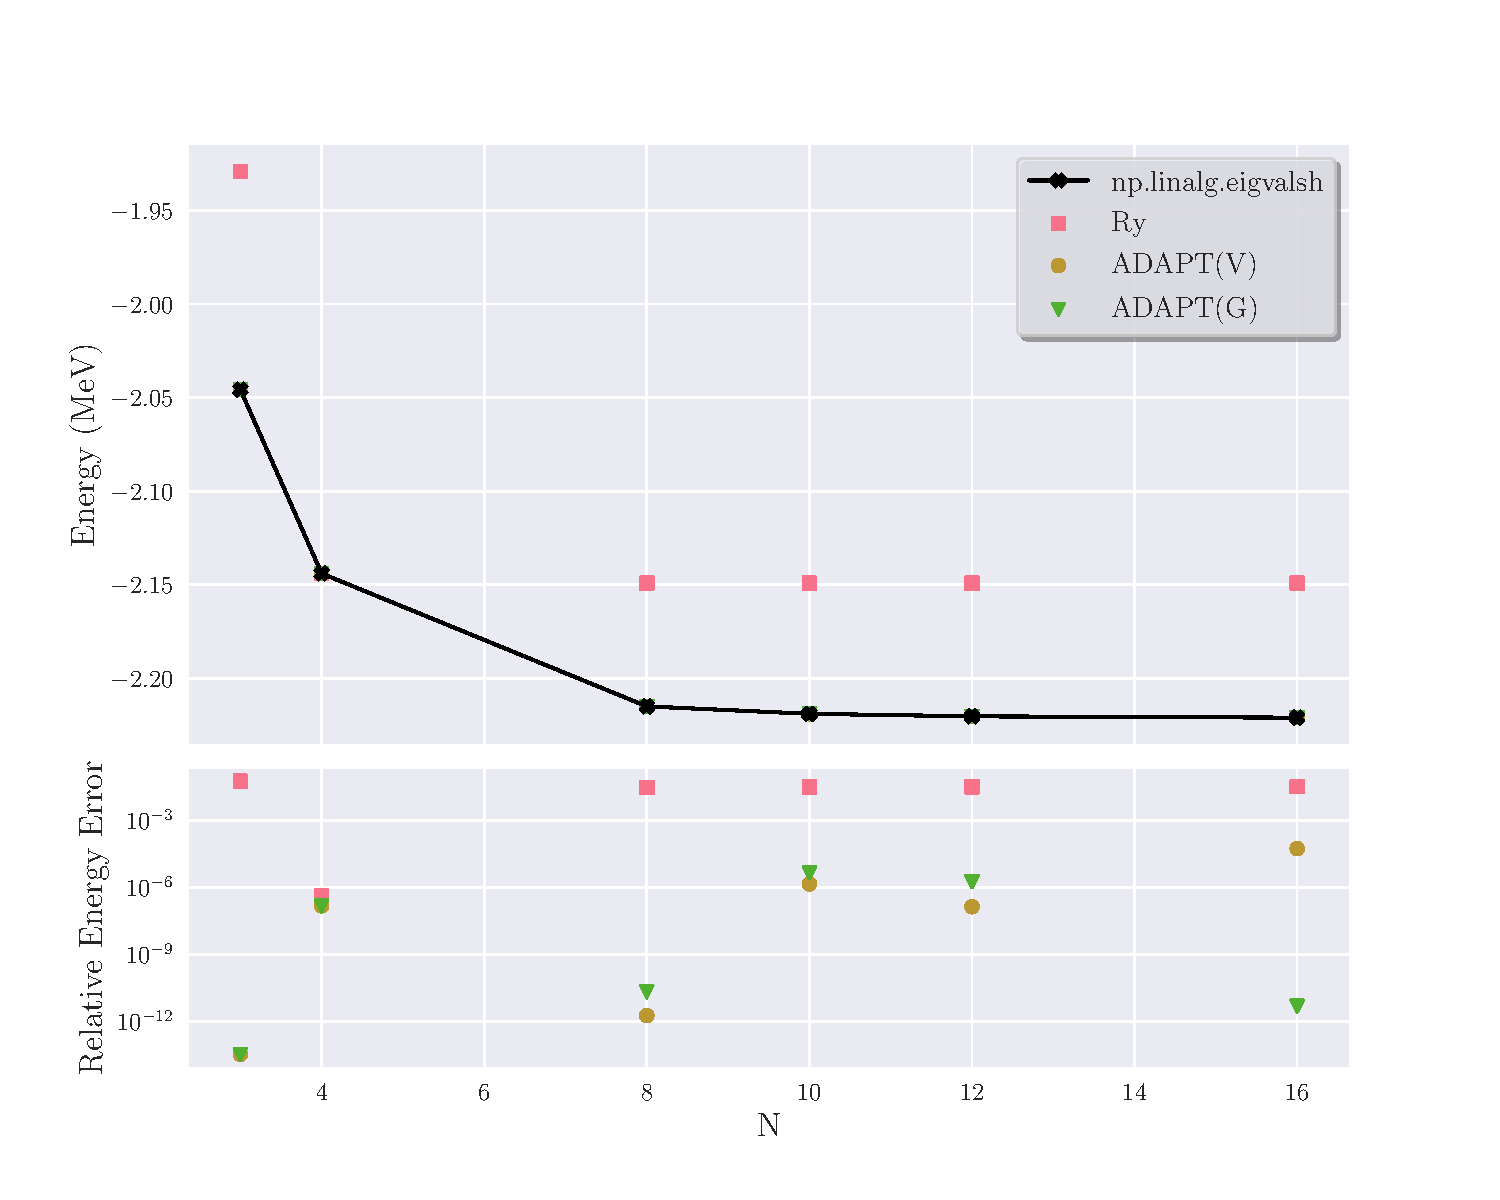
\includegraphics[width=\linewidth]{image/deuteron_result/main1.pdf}
    \caption{The deuteron model with \textbf{exact energy simulation} for $ N \in [3,16] $ with the \texttt{BFGS} optimiser for the ADAPT-VQE for a maximum of $ 16 $ iterations.}
    \label{fig:deuteronmain}
\end{figure}
Again, we saw that the errors obtained using the VQE with hardware efficient ansatz stay around $ 10^{-2} $, even for more qubits. While the ADAPT-VQEs were outperforming the VQE by a large margin for cases with few qubits, as the number of qubits grew, this margin reduced drastically. For $ N=32 $, the ADAPT-VQEs both have errors in orders of $ 10^{-4} $. This is likely due to the fact that as the number of qubits grows, the number of operators needed to represent the ground state also grows. Since the minimum size of a complete pool grows linearly with the number of qubits, the number of operators in the ansatz to represent the ground state should grow linearly as well. We will investigate this further in the Subsection~\ref{sub:itervsqubits}. 

\subsection{Ideal Simulation}
\begin{figure}[ht]
	\centering
	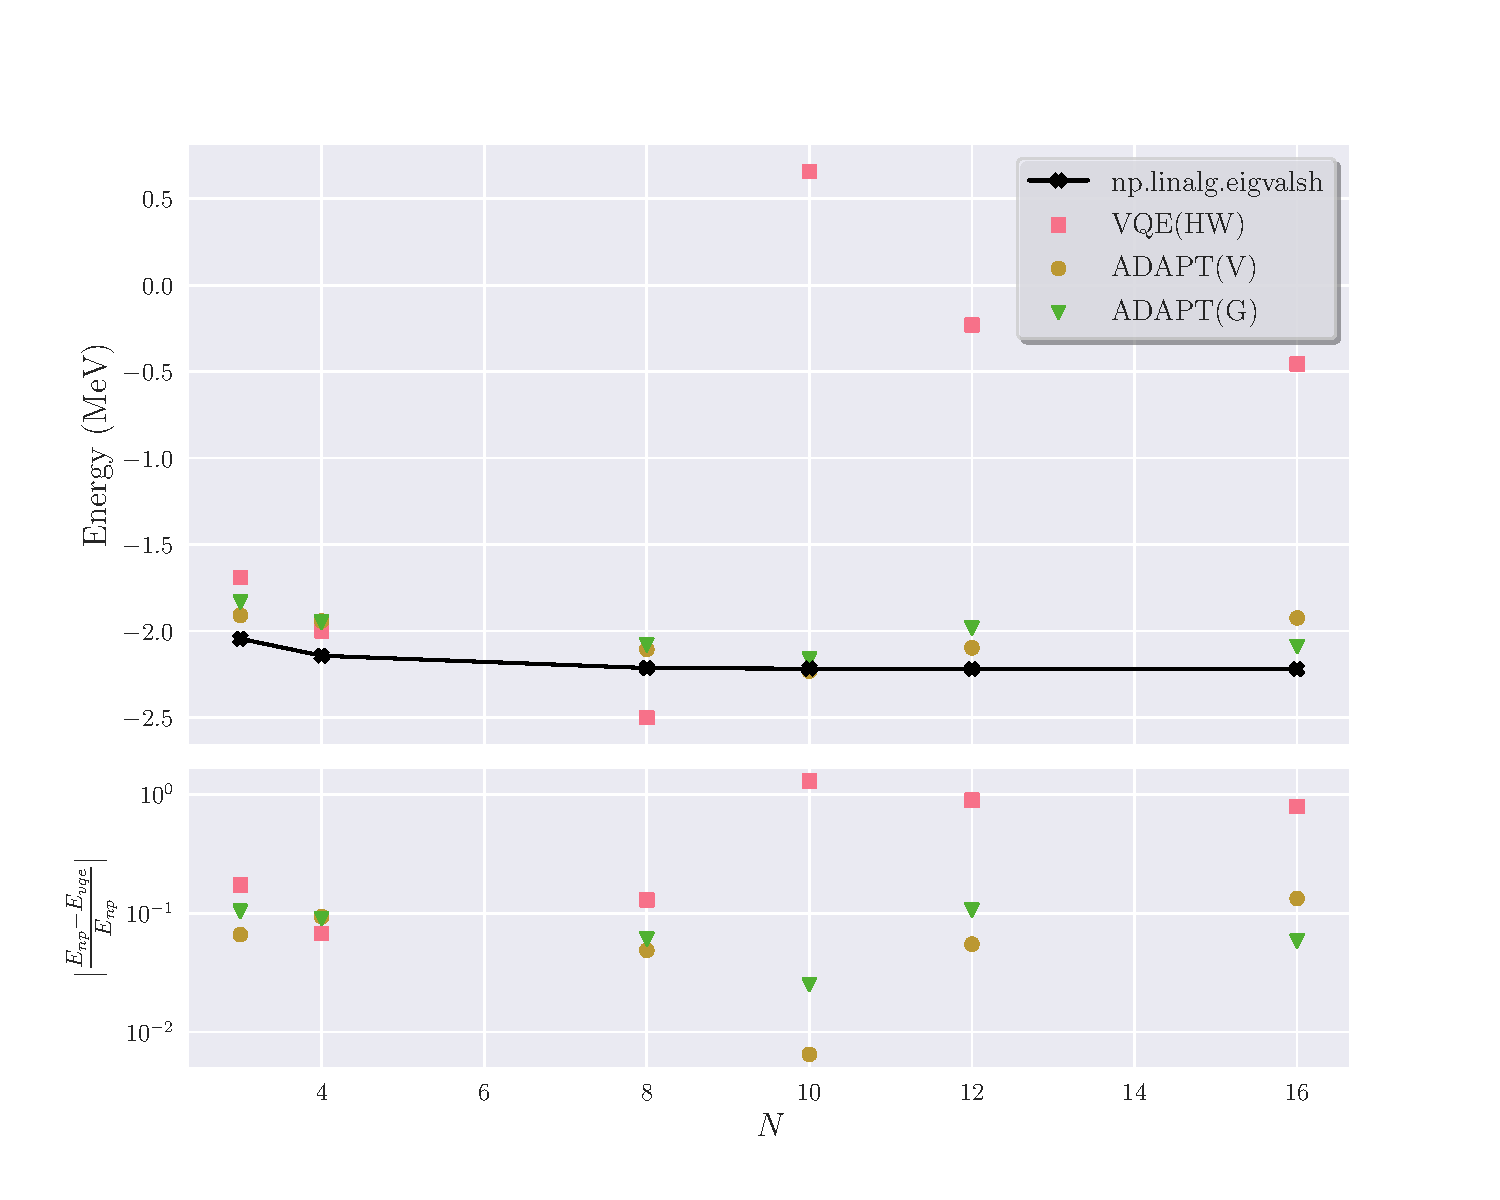
\includegraphics[width=\linewidth]{image/deuteron_result/main2.pdf}
	\caption{The deuteron model with \textbf{ideal simulation} for $ N \in [3, 16] $ with the \texttt{COBYLA} optimiser for the ADAPT-VQE for a maximum of $ 16 $ iterations.}
	\label{fig:deuteronmain-noisy}
\end{figure}

\subsection{Scaling of Iterations with Number of Qubits}
\label{sub:itervsqubits}

How many ADAPT iterations in the exact energy simulation do we expect the qubit-ADAPT-VQE to need to converge? We ran the exact energy simulation for the deuteron model for $ 1 $ to $ 7 $ qubits, using the \texttt{SLSQP} optimiser. The results are shown in Figure~\ref{fig:howmany}. Combining this with Figure~\ref{fig:onlyneed1iter} we could see the number of iterations required for the ADAPT-VQE to converge is independent of the optimisers used but rather the number of the qubits in the system as shown in Figure~\ref{fig:howmany}. We summarised the results in Table~\ref{tab:howmany}. Interestingly, the number of iterations grows much faster for a lower number of qubits, and as the number of qubits increases, the number of iterations required to converge increases at a much slower rate, seemingly linearly. Due to the large amount of time required to run this simulation, we will not be able to run the convergence test for more qubits. However, if the number of iterations required for the convergence does not grow as fast as the number of qubits, then both the QubitAdaptAnsatz and the ADAPT-VQE will scale nicely into larger systems.


\begin{table}[ht]
    \centering
    \caption{Number of iterations required for the ADAPT-VQE to converge for different numbers of qubits.}
    \label{tab:howmany}

    \begin{tabular}{c c c}
	\toprule
	\textbf{N} & \textbf{Number of Qubits} & \textbf{Number of Iterations} \\
	\midrule
	2 & 1 & 1 \\
	4 & 2 & 2 \\
	8 & 3 & 6 \\
	16 & 4 & 8 \\
	32 & 5 & 9 \\
	64 & 6 & 11 \\
	128 & 7 & 12 \\
	\bottomrule
    \end{tabular}
\end{table}
\begin{figure}[ht]
    \centering
    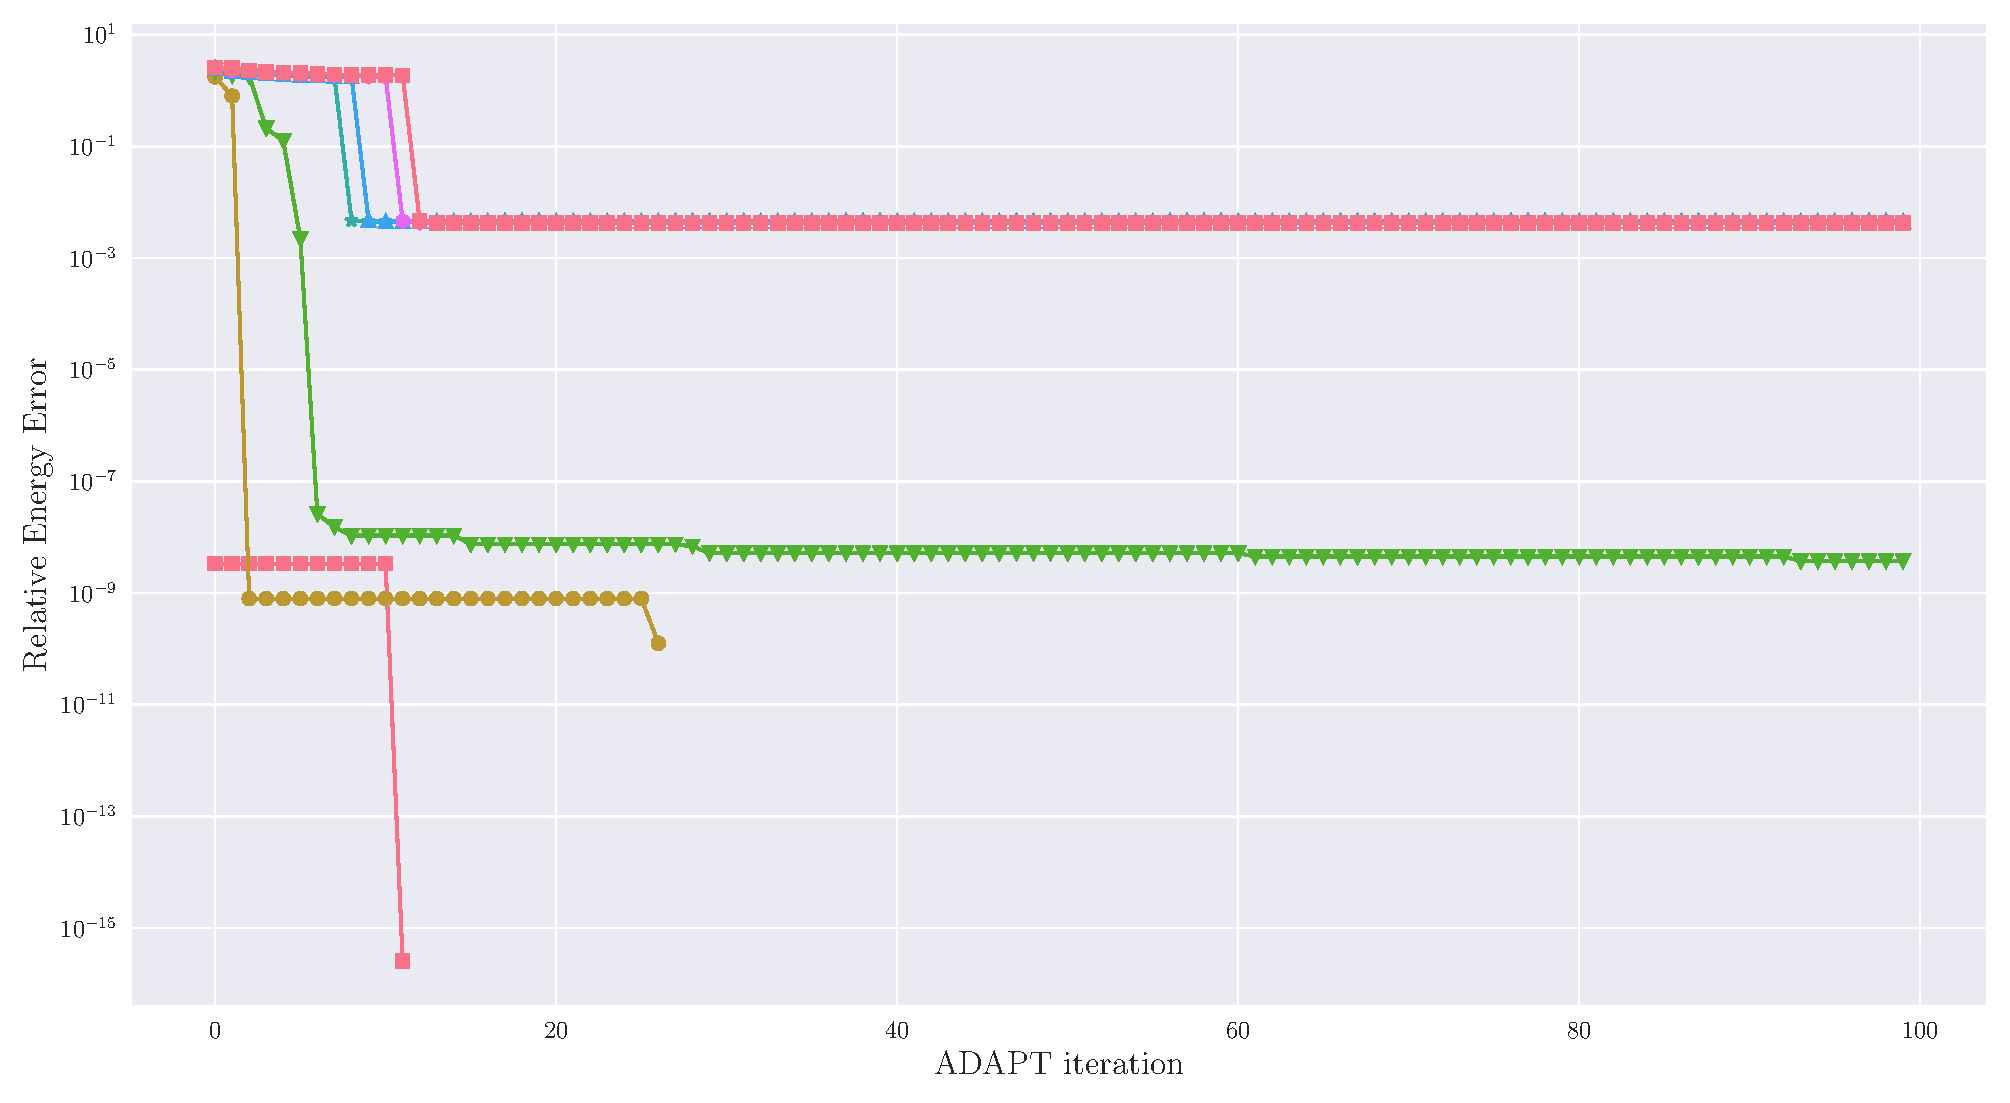
\includegraphics[width=0.8\linewidth]{image/deuteron_result/howmanyiters_whole.pdf}
    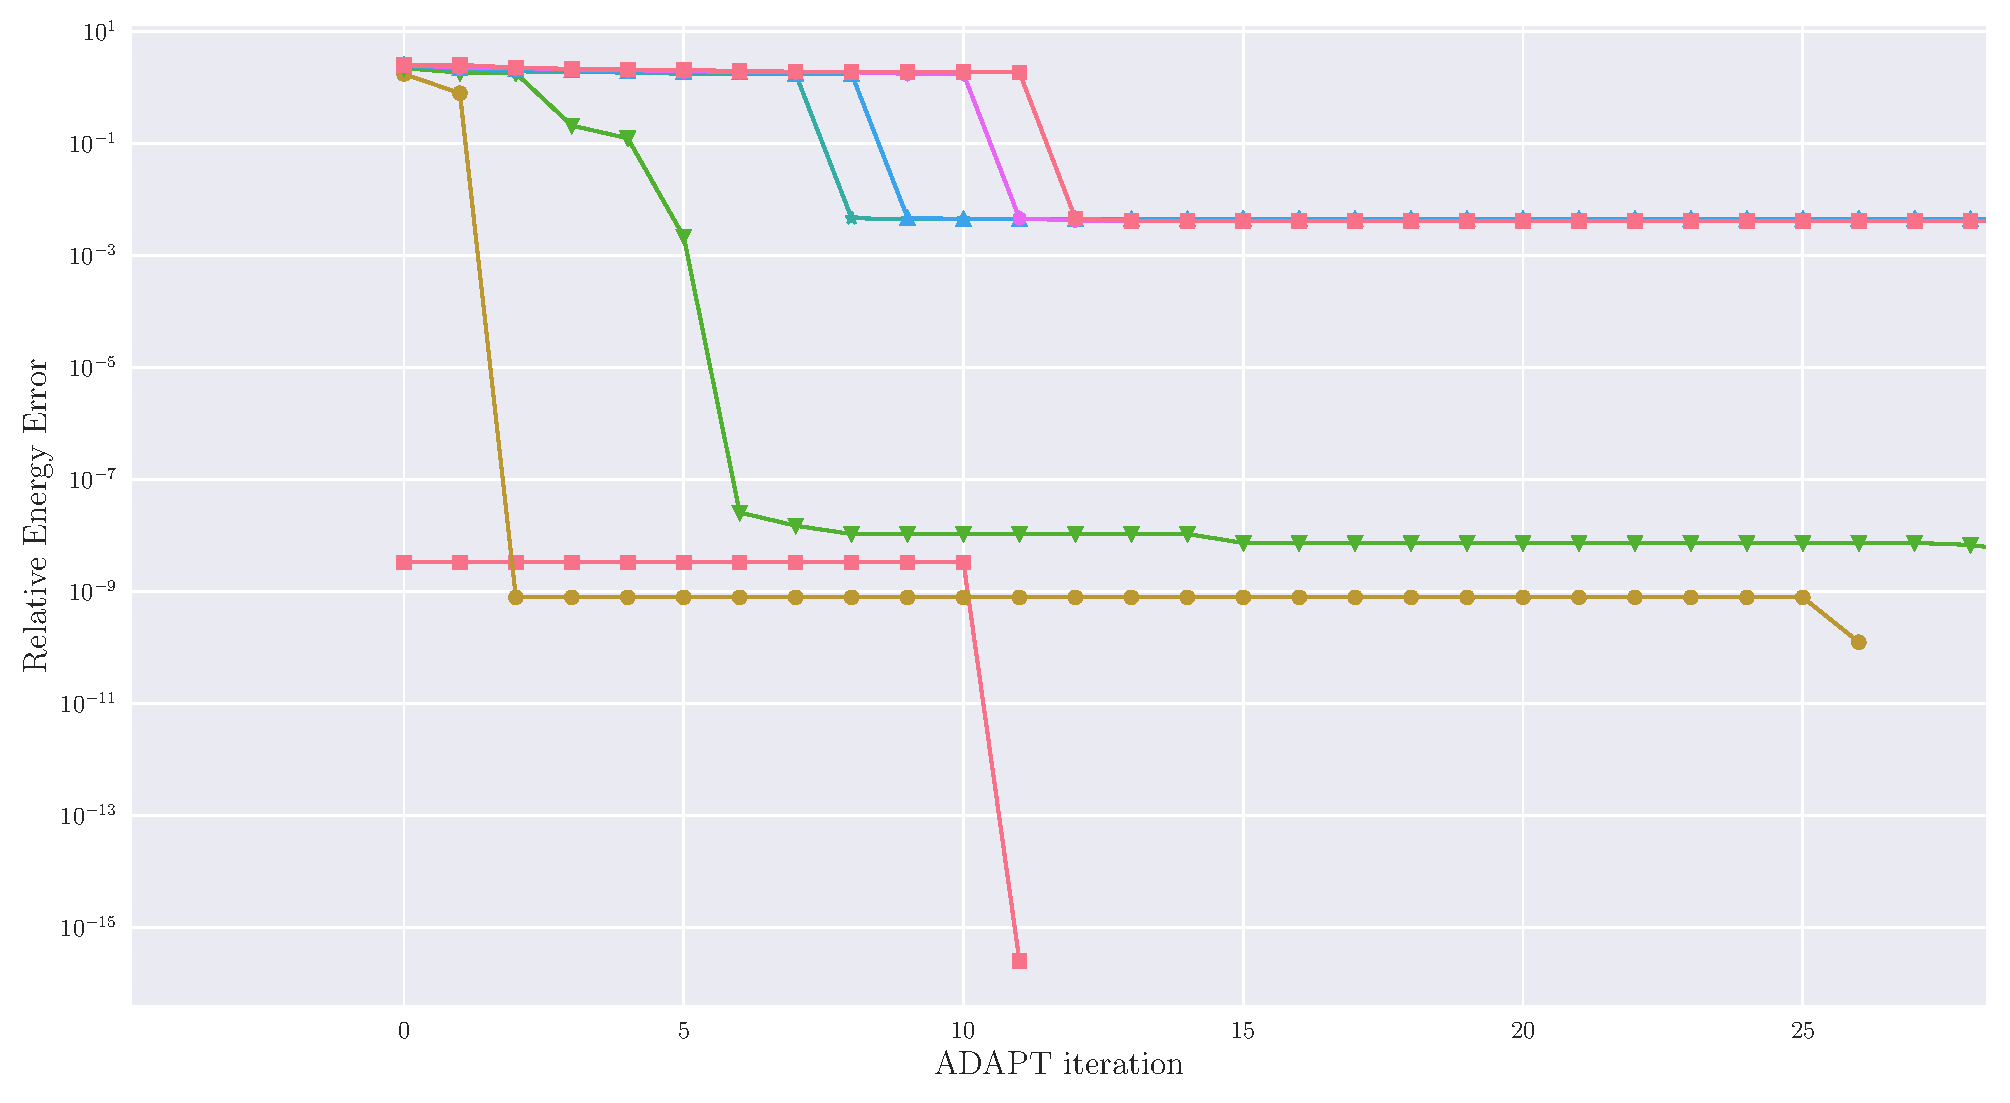
\includegraphics[width=0.8\linewidth]{image/deuteron_result/howmanyiters_zoom.pdf}
    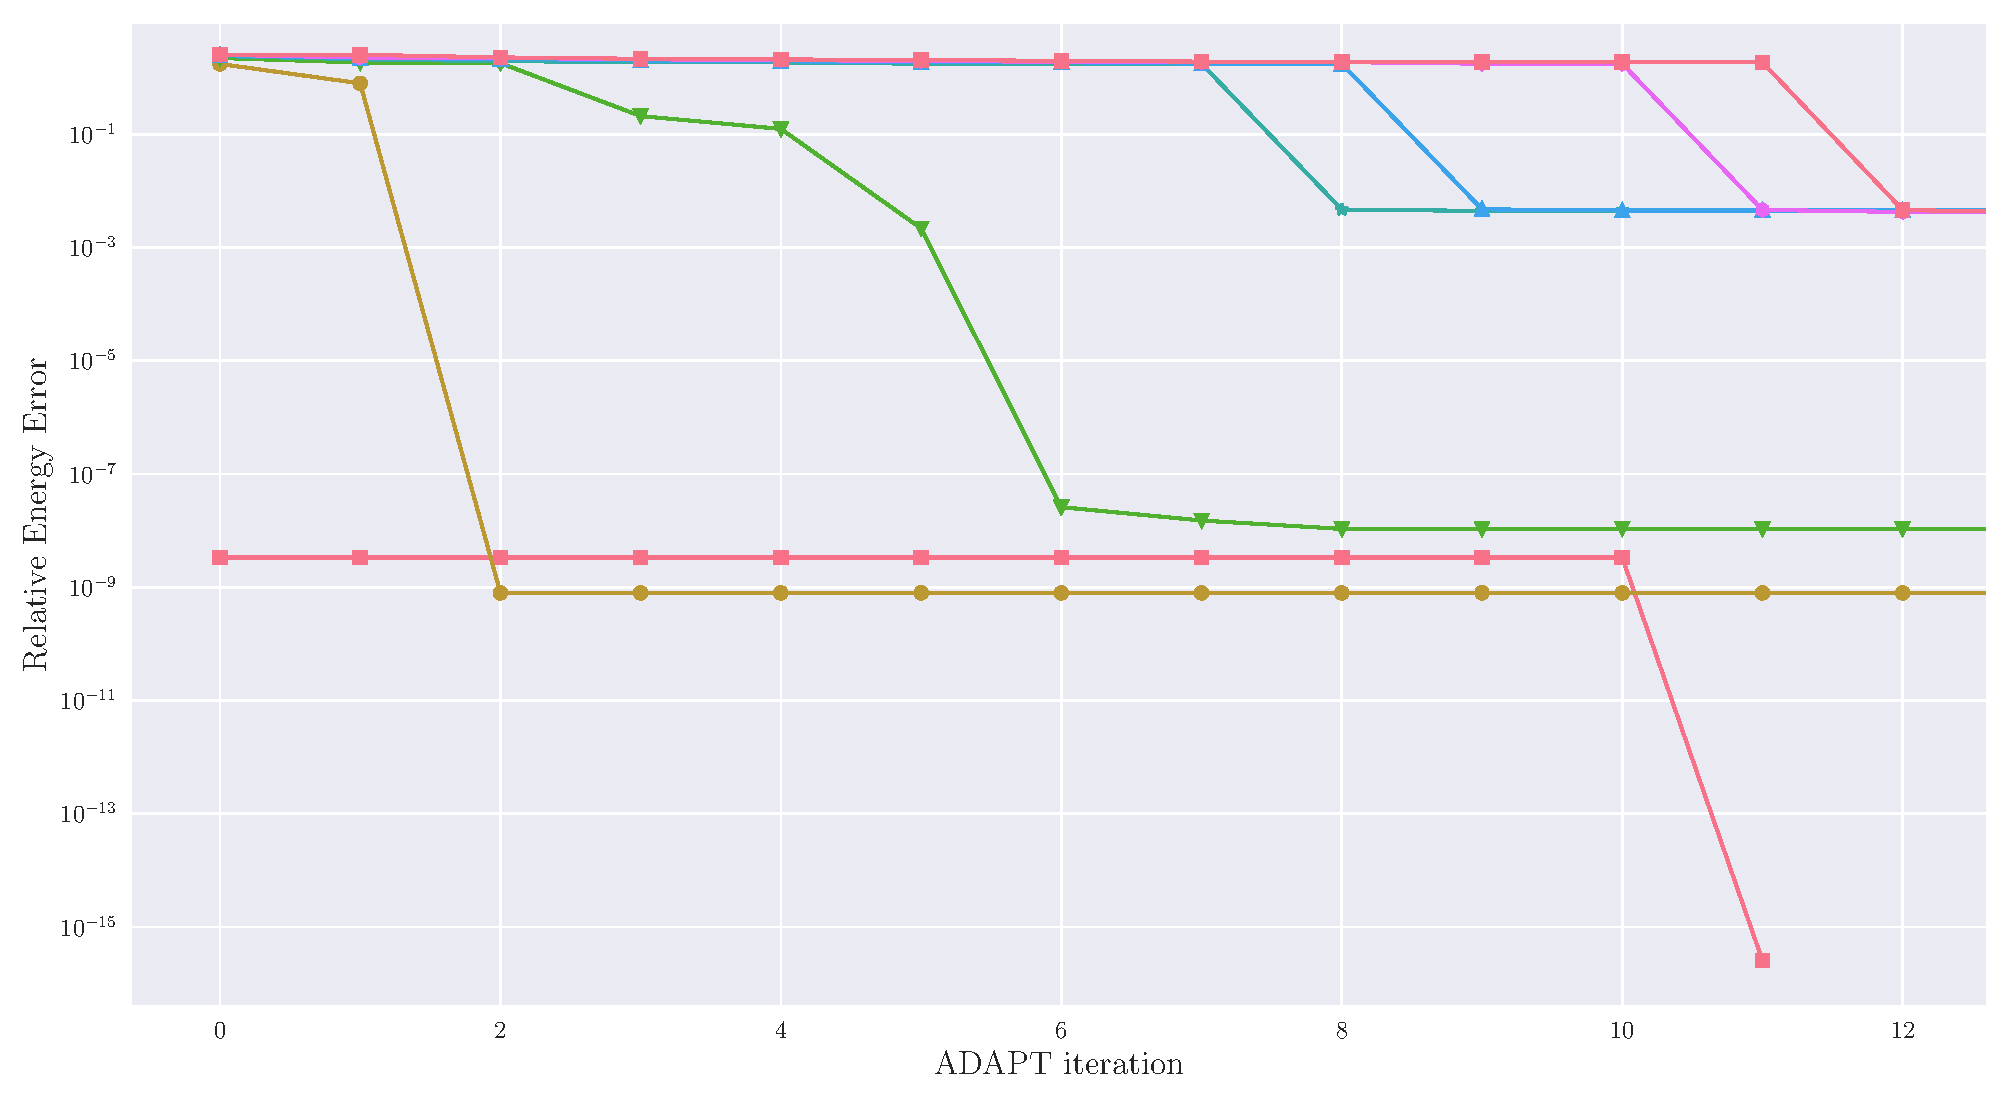
\includegraphics[width=0.7\linewidth]{image/deuteron_result/howmanyiters_zoomzoom.pdf}
    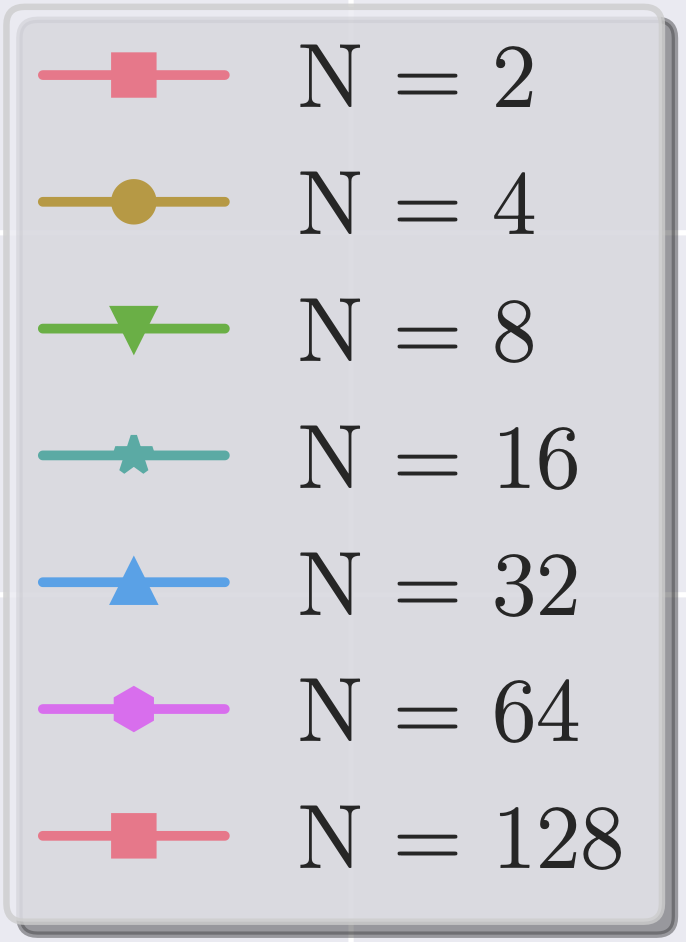
\includegraphics[width=0.2\linewidth]{image/legend.png}
\caption{Number of ADAPT iterations for the deuteron model with exact energy calculation optimised with \texttt{SLSQP}  for $ 1 $ to $ 7 $ qubits with maximum $ 100 $ iterations using the $ G $  pool. The pink line to the left with lower errors corresponds to the $ 1 $ qubit case, and the other pink line corresponds to $ N=128 $, the $ 7 $-qubit case. The top figure shows the whole $ 100 $ iteration, the middle figure shows a zoomed-in version of the top figure for around $ 27 $ iterations, and the bottom figure shows a zoomed-in version of the middle figure for around $ 13 $ iterations.}
    \label{fig:howmany}
\end{figure}

Finally, in an attempt to improve results further, we employed a new initialisation method, where the optimised state from the VQE is used as an initial state of the ADAPT-VQE. This is possible on actual hardware as well, since we know the structure of the ansatz and the optimal parameters. One could simply run the hardware efficient ansatz circuit with the optimal parameters before starting the ADAPT iterations.

\subsection{Initial States}
\label{sub:deuteron_initstate}
The initial state has a significant impact on the convergence of the ADAPT-VQE and VQEs in general. We have found that by utilising the HardwareEfficientAnsatz optimised state as the initial state, the ADAPT-VQE is able to converge to the correct state much faster, as shown in Figure~\ref{fig:whyoptinit}. When a small number of maximum iteration $ (5) $ is used, the ADAPT did not converge to the ground state for more than $ 2 $ qubits due to the limitation on iteration number. However, when the state was initialised with the hardware optimised state, the ADAPT-VQE with both pools converged to the minimum with error to orders of $ 10^{-2} $ or lower, even when the $ Ry $ state did not converge to the minimum. This could be extremely useful as it is usually not expensive in terms of both quantum and classical resources. This is similar to initialising it to the  HF state, except this way we could potentially start in an entangled state which the HF state often is not. We also do not rely on classical many-body methods, which should be preferable.

\begin{figure}[ht]
    \centering
    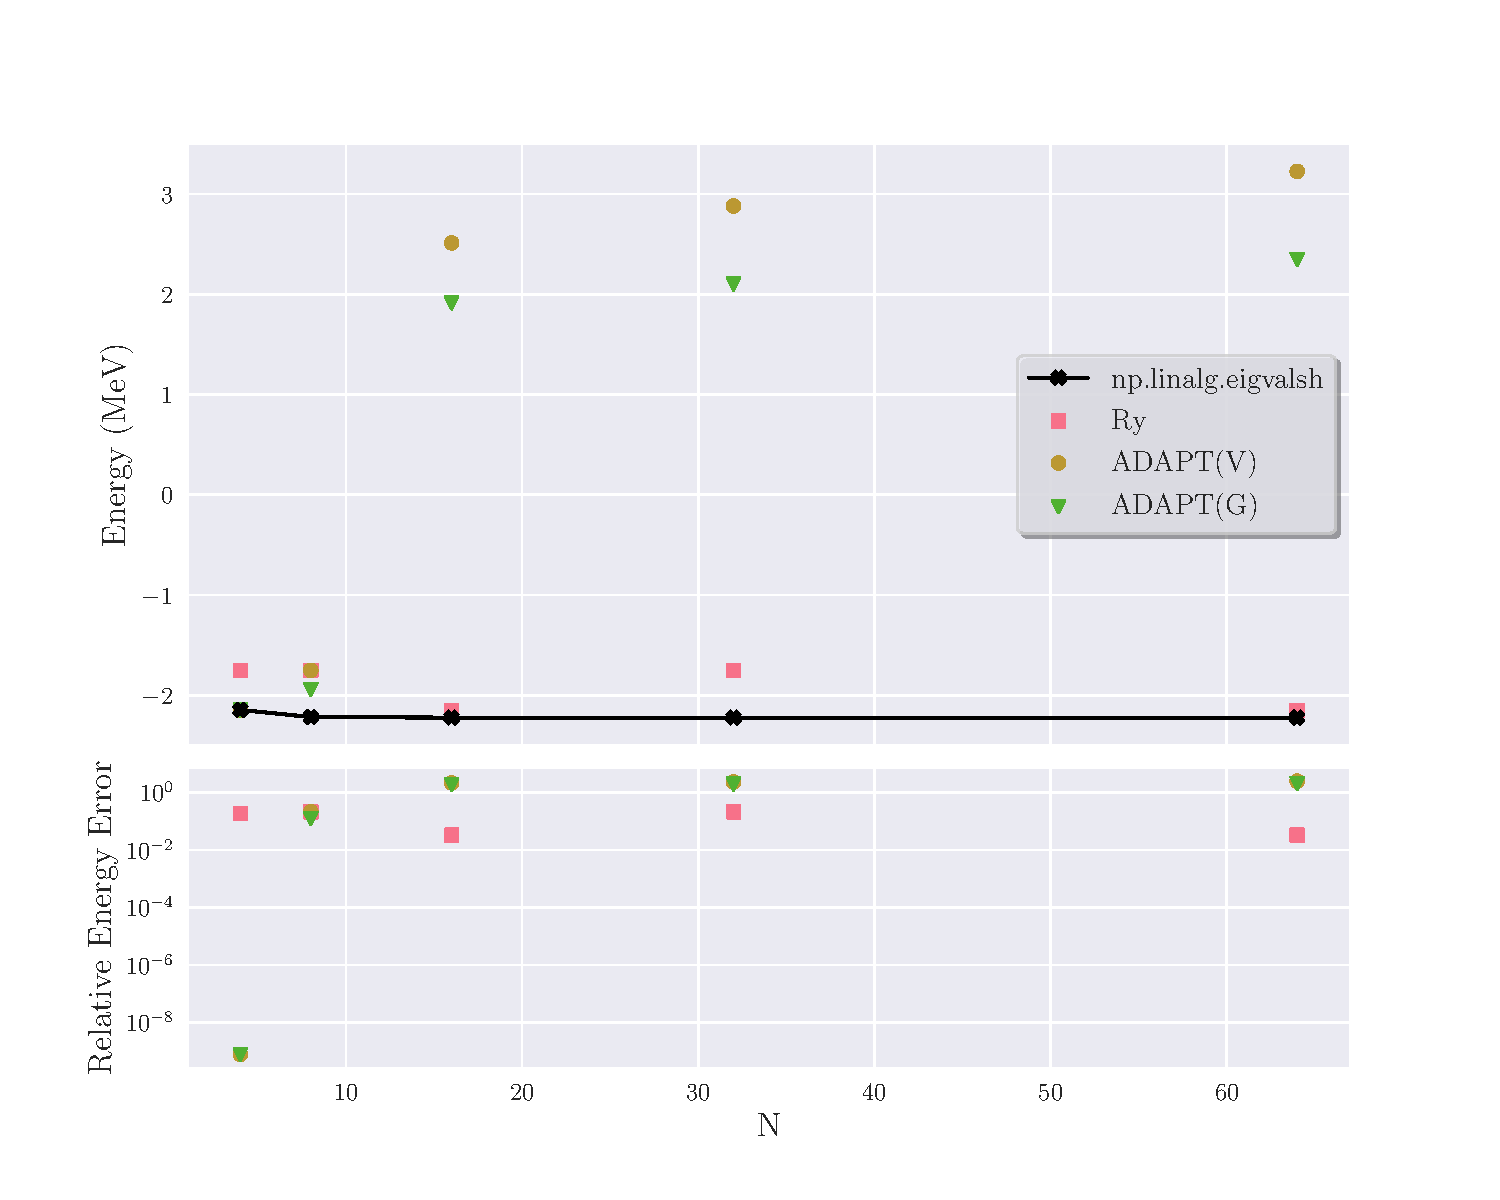
\includegraphics[width=0.8\linewidth]{image/deuteron_result/why_opt_init/S_NE_SLSQP_max_iter=5_hw_rep=2_(2,6,5)deutron_energies.pdf}
    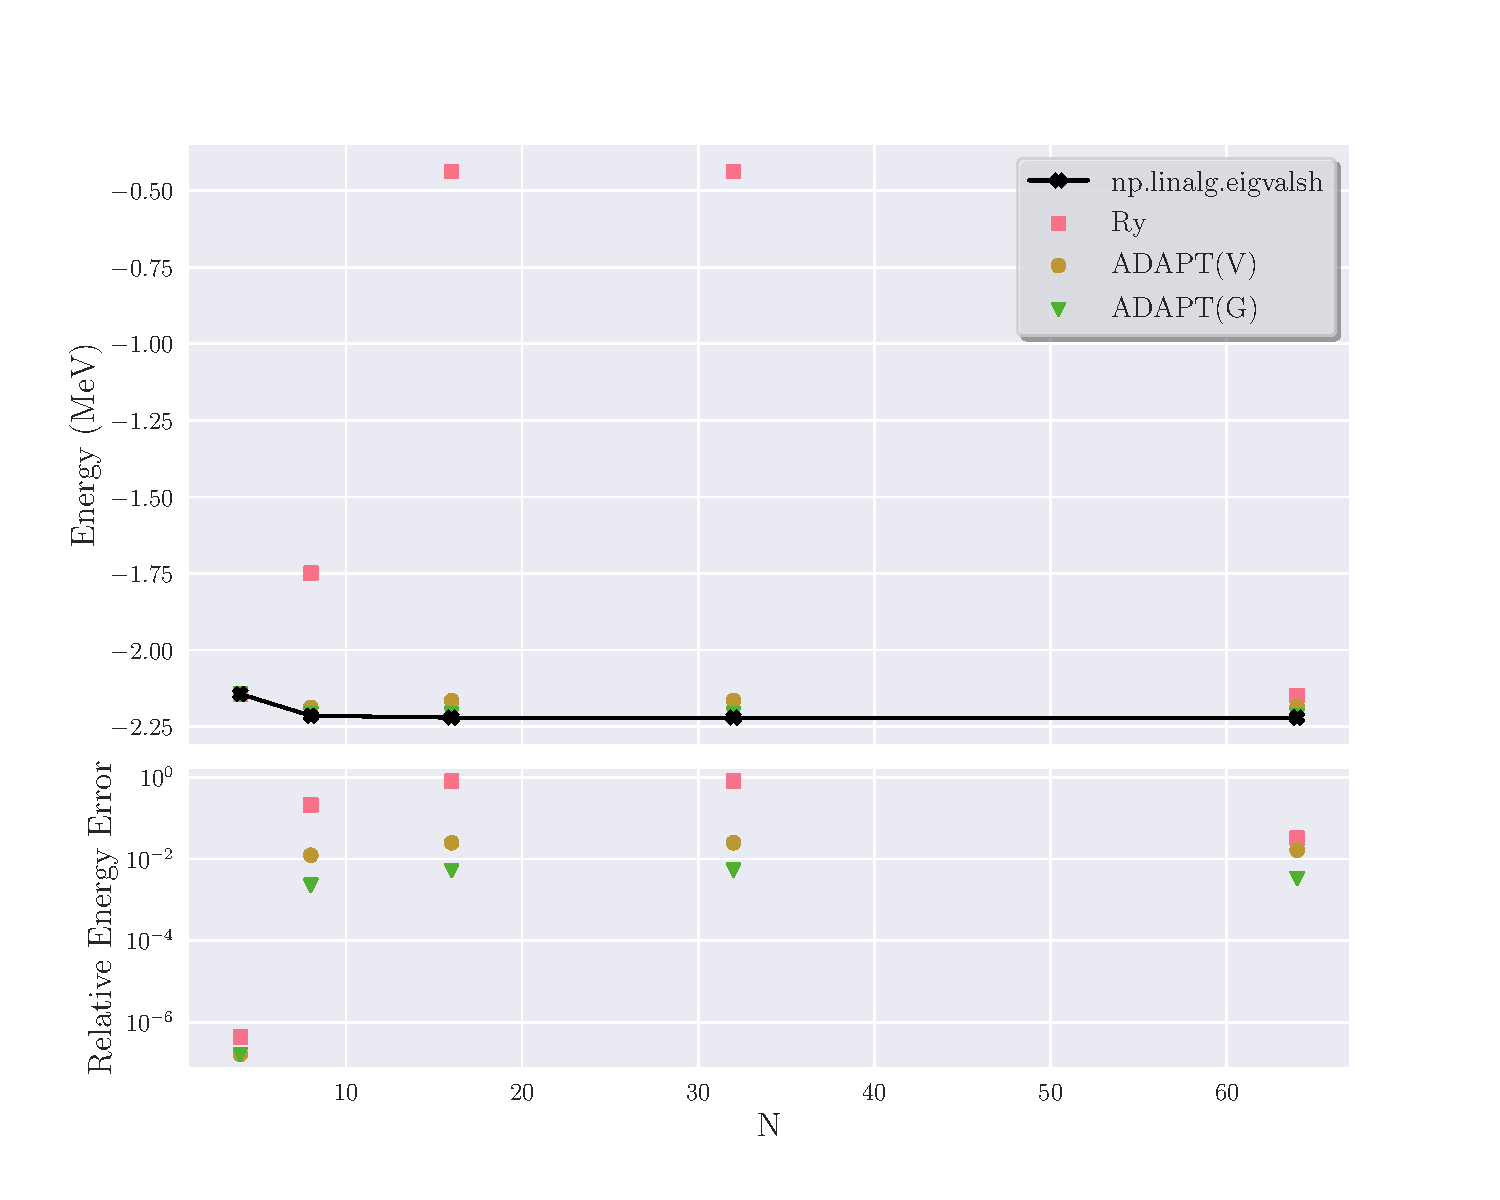
\includegraphics[width=0.8\linewidth]{image/deuteron_result/why_opt_init/S_NE_SLSQP_max_iter=5_hw_rep=2_opt_init_(2,6,5)deutron_energies.pdf}
    \caption{Results obtained for the deuteron Hamiltonian with different basis dimensions $ N $ with \textbf{exact energy calculation} for $ 5 $ maximum iterations and $ 2 $ repetition for the Hardware Efficient Ansatz Ry. The exponentials were decomposed using the \textbf{staircase} algorithm, and both VQEs were optimised with the \texttt{SLSQP} method. The top figure shows the results when the initial state is the maximally superposed state, and the bottom figure shows the results when the initial state is the Hardware Efficient Ansatz optimised state.}
    \label{fig:whyoptinit}
\end{figure}



\chapter{Conclusion}

\section{Summary of Results}
The aim of this thesis project is twofold: to create a quantum computing library that is oriented towards physicists and to study the performance of the Variational Quantum Eigensolver (VQE) and the Adaptive, Problem Tailor (ADAPT) VQE to obtain some insights for the best practices in using these algorithms. 

We built Quanthon as a result, which contains the basic elements to be able to perform any quantum operation. The \texttt{Hamiltonian} class was made to allow the Hamiltonians to be entered in a low-level way by specifying the one- and two-body coefficients. Other functionalities include the \texttt{VQE} and \texttt{ADAPT-VQE} classes which are the main focus of this project, as well as different modules that can assist the quantum simulations, including the mappers to convert fermionic Hamiltonians or matrix Hamiltonians to qubit Hamiltonians, the staircase and inverted staircase algorithms for converting exponentials of Pauli strings to quantum circuits, and the expectation value estimator which simulates the measurements of the quantum circuits and computes the expectation values of the Hamiltonians. 

With the library built, we then proceeded to study the performance of the VQE with hardware efficient ansatzes and ADAPT-VQE with two different minimal complete pools, the $ V $ and the $ G $ pool defined in Subsection~\ref{sub:qubit_adapt_vqe}, through both exact energy and ideal simulations of the multiple models. With the exact energy simulation, we observed that the hardware efficient ansatz in many cases does not converge to the ground state. When it does, the relative error is usually of order $ 10^{-2} $. The ADAPT-VQE with minimal pools, however, can indeed converge to the ground state with relative error lower than $ 10^{-6} $ given enough ADAPT iterations. The number of iterations it takes for the qubit-ADAPT-VQE to converge scales roughly linearly with the number of qubits in the model and the choice of the optimiser is independent of the number of iterations required. The best optimiser for the VQE was found to be the Powell method, and the best optimiser for the qubit-ADAPT-VQE was the BFGS method. 

In the presence of shot noise, the convergence of the qubit-ADAPT-VQE slows down but is still more stable and consistently outperforms the hardware efficient ansatz. We compared the error with the expected error from the number of shots to see if the algorithms have converged. The best optimiser, in this case, is the COBYLA method for the qubit-ADAPT-VQE and the Powell method for the VQE. We noticed that the ADAPT-VQE rarely exits due to the gradient being below the tolerance level, which is likely due to the noise.

No significant differences were observed in the performances of the $ V $ and $ G $ pool, except in the case of large pairing strength the $ G $ pool converges much faster than the $ V $ pool.

Additionally, we found that the gradient for all the operators in the minimal complete pool can be $ 0 $ for many Hamiltonians if the state is initialised in the $ \ket{0} $ state. This causes the ADAPT-VQE to exit immediately without any iterations. Initialising randomly avoids this problem but causes slow convergence. First, we used the maximally superposed state as an initial state. Later, we found that by initialising the ADAPT-VQE with the optimised state from hardware efficient ansatz boosts performances by reducing the number of iterations it takes for the ADAPT-VQE to converge. 

\section{Future Work}

We will group future work into two categories: improvements to the Quanthon library and improvements to the VQE and ADAPT-VQE algorithms.

\subsection{Improvements to Quanthon}
Many functionalities can be added to the Quanthon Library, such as adding more predefined gates or other popular algorithms. We could also explore other mappers, such as the Bravyi-Kitaev transformation~\cite{Seeley2012}. To increase the speed of simulations we could parallelise the measurements and add an option to group commuting terms of the Hamiltonian to be measured simultaneously. Integration with quantum hardware could also be extremely useful to allow the library to run on real quantum devices. More ansatzes could be implemented to allow for flexibility and performance comparison, specifically the unitary coupled cluster ansatz~\cite{Romero2019} and the fermionic-ADAPT ansatz~\cite{grimsley2019}. This would allow for a more comprehensive comparison of the ansatz. Another interesting direction would be to implement noise models to allow for noisy simulations.
\subsection{Improvements to Simulation Results}
The ideal simulation takes a long time to run, therefore the maximum number of iterations was all set to below $ 30 $, the performance of the ADAPT-VQE could potentially be improved by simply allowing the algorithm to run for more iterations. The $ 0 $ gradient problem is also concerning as the initial state could cause the algorithm to exit prematurely. More research is needed to find out under which circumstance would the gradient vanish and come up with either a different operator selection criteria for choosing an operator to be appended to the ansatz, or a systematic way to select the initial state to avoid the difficulty in convergence.



\chapter{}
\section{Left and right eigenvectors and bi-orthogonal sets.}
\label{sec:biort}
Given the eigenvalue equation, 
\begin{equation}
  A^{\mathrm{T}} y = \lambda y, 
\end{equation}
where the $n\times n$ matrix $A^{\mathrm{T}}$ is of general form. The eigenvalues $\lambda $ are 
determined by the characteristic equation,
\begin{equation}
  \mathrm{det}(A^{\mathrm{T}}-\lambda I) = \mathrm{det}(A-\lambda I) = 0,
\end{equation}
which shows that the eigenvalues of $A^{\mathrm{T}}$ are the same
as those of $A$. Consider the eigenvalue equation for the $i$'th 
eigenvector, 
\begin{equation}
  A^{\mathrm{T}} y_i = \lambda_i y_i, 
\end{equation}
then the transpose of this equation gives,
\begin{equation}
  y_i^{\mathrm{T}}A  = \lambda_i y_i^{\mathrm{T}}, 
  \label{eq:left}
\end{equation}
here $y_i^{\mathrm{T}}$ is the left eigenvector of $A$ corresponding
to the eigenvalue $\lambda_i$. The eigenvalue equation for $A$ is 
\begin{equation}
  A x_j = \lambda_j x_j, 
  \label{eq:right}
\end{equation}
where it is seen that $x_j$ is the right eigenvector of the matrix $A$ 
corresponding to the eigenvalue $\lambda_j$.
Now multiply Eq.~(\ref{eq:left}) with $x_j$ from the right and
Eq.~(\ref{eq:right}) with $y_i^{\mathrm{T}}$ from the left, and subtract to obtain,
\begin{eqnarray}
  \lambda_j y_i^{\mathrm{T}}x_j & = & \lambda_i y_i^{\mathrm{T}}x_j, \\
  \Rightarrow \: (\lambda_j -\lambda_i) y_i^{\mathrm{T}}x_j & = & 0, \\
  \Rightarrow \: y_i^{\mathrm{T}}x_j & = & 0 \:\: \mathrm{if} \lambda_i \ne \lambda_j, 
\end{eqnarray}
where it is customary to say that the 
left $y_i^{\mathrm{T}}$  and right $x_j$ eigenvectors of a 
matrix $A$ 
are \emph{bi-orthogonal} to each other.
If all $n$  
eigenvalues of the matrix $A$�are distinct, then
$y_i^{\mathrm{T}}x_j = 0 $ for $i,j = 1,2,...,n, \: i \ne j$, but 
$y_i^{\mathrm{T}}x_i \ne 0 $.  This implies that the right and left 
eigenvectors can be scaled so they form a complete set of \emph{bi-orthogonal} 
vectors.
\begin{equation}
  Y^\mathrm{T} X = \sum_{i,j=1}^n y_i^\mathrm{T}x_i = \sum_{i,j=1}^n\delta_{i,j} = 1.
\end{equation}
Here $Y^\mathrm{T}$ is a matrix whose rows are $y_i^\mathrm{T}, i=1,...,n$�and
$X$�is a matrix whose columns are $x_i, i = 1,...,n$.
This shows explicitly that $Y^\mathrm{T}$ is the inverse of $X$. 
It is clear that this works for any matrix which has a complete 
set of linearly independent eigenvectors (a nondefective matrix) 
regardless of whether the eigenvalues are distinct. 
As we have seen before, we can write in this case
\begin{displaymath}X^{-1}AX=\, {\rm diag}\, [\lambda _i]. \end{displaymath}
Indeed, if we can find any matrix $Z$ such that $Z^{-1}AZ$ is diagonal, 
then the columns of $Z$ are the right eigenvectors of $A$, and the rows of $Z^{-1}$ 
are the left eigenvectors of $A$, 
while the diagonal entries of $Z^{-1}AZ$ are the eigenvalues of $A$.
Defective matrices have an incomplete set of eigenvectors, 
and the theory requires their reduction to Jordan normal form. 

In the special case of $A$ being a complex symmetric matrix, which is
often the case in physical applications, then the left eigenvectors
are just the transpose of the right eigenvectors. In this case it is sufficient to
solve the right eigenvalue equation, and a complete set of \emph{bi-orthogonal} vectors
are obtained directly. 


\section{Three-body matrix elements in $j-j$ coupling} 
\label{sec:3matel}
Throughout this section the anti-symmetric three-, two-body 
wave functions are written as $\bar{\Psi}�$ and $\bar{\Phi}$�
respectively, while the non-anti-symmetrized functions are without 
the bar. The single-particle wave functions are given by $\phi $. 
The anti-symmetric three-body wave function may be written 
\begin{equation}
  \bar{\Psi}_{(ab)c}^{JM}(123) = {1\over \sqrt{3}}\left\{ \Psi_{(ab)c}^{JM}(123) 
  - \Psi_{(ab)c}^{JM}(132) + \Psi_{(ab)c}^{JM}(231) \right\} 
  \label{eq:threebody}
\end{equation}
here $(ab)c$ labels all relevant single particle quantum numbers  
$a = {n_a, l_a,j_a}$, and the coupling rule $\left( j_a\otimes j_b\right) _{J_{ab}}\otimes j_c$  is 
indicated.
The wave function in Eq.~\ref{eq:threebody} is 
anti-symmetric only in case where at least two of the orbits $abc$ are 
different. In the case $a=b=c$ one has to make use of  coefficients of 
fractional parentage to make the three-body wave function anti-symmetric.
 The non anti-symmetrized wave functions 
$ \Psi_{(ab)c}^{JM}(123) $ are given by 
\begin{equation}
  \Psi_{(ab)c}^{JM}(123) = \Psi\left( \bar{\Phi}_{ab}^{J_{ab}}(12)\phi_c(3); JM \right)
\end{equation}
Here $ \bar{\Phi}_{ab}^{J_{ab}}(12) $ is an anti-symmetric two-particle wave function.
\begin{equation}
  \bar{\Phi}_{ab}^{J_{ab}}(12) = {1\over \sqrt{ 2 (1+\delta_{ab})}}\sum_{m_a,m_b} 
  \langle j_a m_a, j_b m_b \vert J_{ab} M_{ab}\rangle \left( \phi_a(1) \phi_b(2) - \phi_a(2)\phi_b(1)\right)
\end{equation}
In the following derivation the total spin and projection $JM$ will 
be suppressed for notational economy. 

Consider a matrix element of the three-body wave function in Eq.~\ref{eq:threebody}
with a general interaction consisting of only two-body terms $V= V_{12} +V_{13}+V_{23}$.
\begin{eqnarray}
  \langle \bar{\Psi}_{(ab)c}(123) \vert V \vert \bar{\Psi}_{(de)f}(123)\rangle = \\
	  {1\over \sqrt{3}}\langle \Psi_{(ab)c}(123) 
	  - \Psi_{(ab)c}(132) + \Psi_{(ab)c}(231) \vert V \vert \bar{\Psi}_{(de)f}(123)\rangle
\end{eqnarray}
from the anti-symmetry follows
\begin{eqnarray}
  \langle {\Psi}_{(ab)c}(123) \vert V  \vert \bar{\Psi}_{(de)f}(123)\rangle & = &  
  \langle -{\Psi}_{(ab)c}(131) \vert V\vert \bar{\Psi}_{(de)f}(123)\rangle  \\
 & = & \langle {\Psi}_{(ab)c}(231) \vert V\vert \bar{\Psi}_{(de)f}(123)\rangle 
\end{eqnarray} 
and henceforth
\begin{eqnarray}
  \langle \bar{\Psi}_{(ab)c}(123) \vert V \vert \bar{\Psi}_{(de)f}(123)\rangle  =
  \sqrt{3}\langle {\Psi}_{(ab)c}(123) \vert V \vert \bar{\Psi}_{(de)f}(123)\rangle = \\
  \langle {\Psi}_{(ab)c}(123) \vert V_{12}\vert \Psi_{(de)f}(123)-\Psi_{(de)f}(132)+\Psi_{(de)f}(231)\rangle + \\
  2\langle {\Psi}_{(ab)c}(123)\vert V_{23}\vert \Psi_{(de)f}(123)-\Psi_{(de)f}(132)+\Psi_{(de)f}(231)\rangle 
  \label{eq:matel1}
\end{eqnarray}
Starting with the matrix element of $V_{12}$, one has
\begin{equation}
  \langle {\Psi}_{(ab)c}(123) \vert V_{12} \vert \Psi_{(de)f}(123)-\Psi_{(de)f}(132)+\Psi_{(de)f}(231)\rangle =
  V_{12}^1 + V_{12}^2 + V_{12}^3
  \label{eq:v12}
\end{equation}
where
\begin{equation}
  V_{12}^1 = \langle ab \vert V_{12} \vert  de \rangle^{AS}_{J_{ab}} \:\delta_{c,f}\:\delta_{J_{ab},J_{de}}
\end{equation}
and
\begin{equation}
  V_{12}^2+V_{12}^3 = \langle {\Psi}_{(ab)c}(123) \vert V_{12} \vert 
  -\left( \Psi_{(de)f}(132) - \Psi_{(de)f}(231) \right) \rangle
\end{equation}
recoupling $1,3 \rightarrow 1,2 $ in  $ \Psi_{(de)f}(132) $ and 
$ 2,3 \rightarrow 2,1 $ in $ \Psi_{(de)f}(231)  $ one may show by 
angular momentum algebra that 
\begin{eqnarray}
 -  \left( \Psi_{(de)f}(132) - \Psi_{(de)f}(231) \right) = \\
 \left( {1+\delta_{d,f} \over 1 + \delta_{d,e}} \right)^{1/2} \sum_{J_{df}} 
  (-1)^{j_d + J_{df}-J_{de}-J}U(j_e\:j_d\:J\:j_f; J_{de}\:J_{df})\Psi_{(df)e}(123) \\
  -\left( {1+\delta_{e,f} \over 1 + \delta_{d,e}} \right)^{1/2} \sum_{J_{ef}} 
  (-1)^{j_d + J_{ef}-J}U(j_d\:j_e\:J\:j_f; J_{de}\:J_{ef})\Psi_{(ef)d}(123) 
\end{eqnarray}
here $U(j_a\:j_b\:J\:j_c; J_{ab}\:J_{bc}) $ are the normalized Racah coefficients. 
It follows that the terms $V_{12}^2 $ and $V_{12}^3$ are given by
\begin{eqnarray}
  \nonumber
  V_{12}^2 = \left( {1+\delta_{d,f} \over 1 + \delta_{d,e}} \right)^{1/2} \sum_{J_{df}} 
  (-1)^{j_d + J_{df}-J_{de}-J}U(j_e\:j_d\:J\:j_f; J_{de}\:J_{df}) \times\\
  \langle ab\vert V_{12}\vert df\rangle_{J_{ab}}^{AS}\:\delta_{c,e}\delta_{J_{ab},J_{df}} \\
  \nonumber
  V_{12}^3 = - \left( {1+\delta_{e,f} \over 1 + \delta_{d,e}} \right)^{1/2} \sum_{J_{ef}} 
  (-1)^{j_d + J_{ef}-J}U(j_d\:j_e\:J\:j_f; J_{de}\:J_{df}) \times \\
  \nonumber
  \langle ab\vert V_{12}\vert ef\rangle_{J_{ab}}^{AS}\:\delta_{c,d}\delta_{J_{ab},J_{ef}} \\
\end{eqnarray}
Calculating the matrix element of $V_{23}$ one first recouple $1,2 \rightarrow 2,3$ in
the $\langle \mathrm{bra} \vert$.
\begin{eqnarray}
  \Psi_{(ab)c}(123) = \left( { 1\over 2(1+\delta_{a,b})} \right) \times \\
  \left\{ 
  \sum_{J_{bc}}(-1)^{j_a+J_{bc}-J}U(j_aj_bJj_c; J_{ab}J_{bc}) 
  \Psi\left( \Phi_{bc}^{J_{bc}}(23)\phi_a(1) \right) + \right. \\
    \left. \sum_{J_{ac}}(-1)^{j_a-J_{ab}+J_{ac}-J} U(j_b j_a J j_c; J_{ab} J_{ac}) 
  \Psi\left( \Phi_{ac}^{J_{ac}}(23)\phi_b(1)\right) \right\}
\end{eqnarray}
here $ \Phi_{bc}^{J_{bc}} $ and $ \Phi_{ac}^{J_{ac}} $ are non anti-symmetric two-body wave functions.
Anti-symmetric two-body matrix elements may be expressed in terms non anti-symmetric 
matrix elements by
\begin{equation}
\langle\bar{\Phi}_{ab}(12) \vert V_{12} \vert \bar{\Phi}_{cd}(12) \rangle = 
\left( {2\over (1+\delta_{ab})} \right)^{1/2}
\langle\Phi_{ab}(12) \vert V_{12} \vert \bar{\Phi}_{cd}(12) \rangle 
\end{equation}
Evaluating the matrix element of $V_{23}$ one has to evaluate the following 
matrix elements
\begin{equation}
  \langle \Psi_{(bc)a}(231) \vert V_{23} \vert \Psi_{(de)f}(123)-\Psi_{(de)f}(132)+\Psi_{(de)f}(231)\rangle
\end{equation}
and  
\begin{equation}
  \langle \Psi_{(ac)b}(231) \vert V_{23} \vert \Psi_{(de)f}(123)-\Psi_{(de)f}(132)+\Psi_{(de)f}(231)\rangle
\end{equation}
which are evaluated in the same manner as the evaluation of $V_{12}$ in Eq.~\ref{eq:v12}. 
After some angular momentum recoupling algebra in the $\vert \mathrm{ket}\rangle $, one 
ends up with the final expressions
\begin{eqnarray}
  \nonumber
  \langle \bar{\Psi}_{(ab)c}(123) \vert V \vert \bar{\Psi}_{(de)f}(123)\rangle  =
  \nonumber
  \langle ab \vert V_{12} \vert  de \rangle^{AS}_{J_{ab}} \:\delta_{c,f}\:\delta_{J_{ab},J_{de}} + \\
  \nonumber 
  \left( {1+\delta_{d,f} \over 1 + \delta_{d,e}} \right)^{1/2} 
  (-1)^{j_d - J_{de}+J_{ab}-J}U(j_ej_d J j_f; J_{de} J_{ab}) 
  \langle ab\vert v_{}\vert df\rangle_{J_{ab}}^{AS}\:\delta_{c,e} - \\
  \nonumber
  \left( {1+\delta_{e,f} \over 1 + \delta_{d,e}} \right)^{1/2} 
  (-1)^{j_d + J_{ab}-J}U(j_d j_e J j_f; J_{de} J_{ab}) 
  \langle ab\vert v_{}\vert ef\rangle_{J_{ab}}^{AS}\:\delta_{c,d} + \\
  \nonumber
  \left( { 1+\delta_{b,c} \over 1+\delta_{a,b} } \right)^{1/2}(-1)^{j_a+J_{de}-J}
  U(j_a j_b J j_c; J_{ab} J_{de})   
  \langle  bc \vert v_{} \vert de\rangle_{J_{de}}^{AS}\delta_{a,f} +  \\
  \nonumber
  \left( {1+\delta_{b,c}\over 1+\delta_{a,b} } \right)^{1/2}\sum_{J_{bc}}(-1)^{j_a+j_d-2J} 
  U(j_a j_b J j_c; J_{ab} J_{bc})   \times \\ 
  \nonumber
  \left\{ \left( {1+\delta_{d,f}\over 1+\delta_{d,e} } \right)^{1/2}(-1)^{J_{de}}
  U(j_e j_d J j_f; J_{de} J_{bc}) \langle bc \vert v_{} \vert df \rangle_{J_{bc}}^{AS}\delta_{a,e} + \right. \\ 
  \nonumber
  \left.
  \left( {1+\delta_{e,f}\over 1+\delta_{d,e}} \right)^{1/2}
  U(j_d j_e J j_f; J_{de} J_{bc}) \langle bc \vert v_{} \vert ef \rangle_{J_{bc}}^{AS}\delta_{a,d} \right\}
  + \\ 
  \nonumber
  \left( {1+\delta_{a,c}\over 1+\delta_{a,b}} \right)^{1/2}(-1)^{j_a-J_{ab}+J_{de}-J}
  U(j_b j_a J j_c; J_{ab} J_{de})   
  \langle  ac \vert v_{} \vert de\rangle_{J_{de}}^{AS}\delta_{b,f} +  \\
  \nonumber
  \left( {1+\delta_{a,c}\over 1+\delta_{a,b}} \right)^{1/2}\sum_{J_{ac}}(-1)^{j_a+j_d-J_{ab}-2J} 
  U(j_b j_a J j_c; J_{ab} J_{ac})   \times \\ 
  \nonumber
  \left\{ \left( { 1+\delta_{d,f}\over 1+\delta_{d,e}} \right)^{1/2}(-1)^{J_{de}}
  U(j_e j_d J j_f; J_{de} J_{ac}) \langle ac \vert v_{} \vert df \rangle_{J_{ac}}^{AS}\delta_{b,e} + \right. \\ 
  \left.
  \left( {1+\delta_{e,f}\over 1+\delta_{d,e}} \right)^{1/2}
  U(j_d j_e J j_f; J_{de} J_{ac}) \langle ac \vert v_{} \vert ef \rangle_{J_{ac}}^{AS}\delta_{b,d} \right\}
  \label{eq:matel2}
\end{eqnarray} 
In the case $ a = b = d = e \neq c = f $ and $ J_{ab} = J_{aa}, J_{de}={J'}_{aa}$
are even, Eq.~\ref{eq:matel2} simplifies to 
\begin{eqnarray}
  \nonumber
  \langle \bar{\Psi}_{(aa)c}(123) \vert V \vert \bar{\Psi}_{(aa)c}(123)\rangle  =
  \nonumber
  \langle aa \vert v \vert  aa \rangle^{AS}_{J_{aa}} \:\delta_{J_{aa},{J'}_{aa}} + \\
  \nonumber
  2\sum_{J_{ac}}(2J_{ac}+1) \sqrt{(2J_{aa}+1)(2{J'}_{aa} +1)} 
  \left\{ \begin{array}{ccc}
    j_a & j_a & J_{aa} \\
    j_c & J & J_{ac}�
  \end{array}\right\}
  \left\{ \begin{array}{ccc}
     j_a & j_a & {J'}_{aa} \\
    j_c & J & J_{ac}�
  \end{array}\right\}
  \langle ac \vert v \vert ac\rangle_{J_{ac}} 
\end{eqnarray}
where the normalized Racah coefficients are expressed in terms of $6-j$ symbols.
Next consider the case where all the single particle orbits in the ket are equivalent, 
i.e. $ d = e = f$,  in this case one has to make a coefficients of fractional parentage
expansion to make the three-body wave function totally anti-symmetric in the $j-j$ coupling
scheme;
\begin{equation}
  \bar{\Psi}_{ddd}(123) = \sum_K  \left. \langle j_d^2 K, j_d\vert \right\} j_d^3 J\rangle 
  \Psi_{(dd)d}(123)
\end{equation}
In this way the wave function is expressed in terms of anti-symmetric two-particle 
wave functions, and one may proceed in the same manner as for the case considered above. 
After some angular momentum recouplings, one ends up with the final 
expression for the matrix element,
\begin{eqnarray}
  \nonumber
  \langle \bar{\Psi}_{(ab)c}(123) \vert V \vert \bar{\Psi}_{(dd)d}(123)\rangle  =
  \nonumber
  \sqrt{3} \left. \langle j_d^2 J_{ab}, j_d\vert \right\} j_d^3 J\rangle  
  \langle ab \vert v \vert  dd \rangle^{AS}_{J_{ab}} \delta_{c,d} + \\
  \nonumber
  \sqrt{3}(-1)^{j_a+j_d-2J}
  \sum_K \left. \langle j_d^2 K, j_d\vert \right\} j_d^3 J\rangle \times \\
  \nonumber
  \left\{ \left( {1+\delta_{b,c}\over 1+\delta_{a,b}} \right)^{1/2} 
  \sum_{J_{bc}} U(j_a j_b J j_c; J_{ab} J_{bc})U(j_d j_dJ j_d; K J_{bc}) 
  \langle bc\vert v \vert dd\rangle_{J_{bc}}\delta_{a,d} \right. + \\
  \left. \left( {1+\delta_{a,c}\over 1+\delta_{a,b}} \right)^{1/2} 
  \sum_{J_{ac}} (-1)^{J_{ab}} U(j_b j_a J j_c; J_{ab} J_{ac})U(j_d j_dJ j_d; K J_{ac}) 
  \langle ac\vert v \vert dd\rangle_{J_{bc}}\delta_{b,d} \right\}
\end{eqnarray}




\backmatter{}
\printbibliography{}
\end{document}

